\documentclass[a4paper, 12pt]{book}
\usepackage[utf8]{inputenc}
\usepackage{graphicx}
\usepackage{amsmath, amsthm, amssymb, amsfonts}
\usepackage{gensymb}
\usepackage{tikz}
\usepackage{multicol,lipsum}
\usepackage{hyperref}
\usepackage{pdfpages}
\usepackage{pstricks-add,pst-tools}
\usetikzlibrary{calc,intersections,through,backgrounds,shapes}


\newtheorem{teo}{Teorema}
\newtheorem{defi}{Definição}
\newtheorem{exe}{Exemplo}

\newcommand{\uvec}[1]{\boldsymbol{\hat{\textbf{#1}}}}
\numberwithin{equation}{section}
%\renewcommand{\theequation}{nova configuração}


\title{Minhas aulas}
\author{Antônio Marcos Barbosa}
%\date{Today}


\columnsep=.6cm %Espaçamento entre as colunas
\hoffset=-2cm %Recuo do texto
\textwidth=17.5cm %Largura do texto
\begin{document}

\maketitle
\tableofcontents

%AUXILIO PEDAGÓGICO
%\chapter{PCN}
%http://portal.mec.gov.br/seb/arquivos/pdf/livro03.pdf
%Resumo http://www.somatematica.com.br/artigos/a3/
Os Parâmetros Curriculares Nacionais é umdocumento público que orienta aos professores como ministrarem aulas para os anos iniciais do Ensino Fundamental de forma a obter metas qualitativas determinadas.

''É importante destacar que a Matemática deverá ser vista pelo aluno como um conhecimento que pode favorecer o desenvolvimento do seu raciocínio, de sua sensibilidade expressiva, de sua sensibilidade estética e de sua imaginação'' (PCN's,1997)

\section{Alguns caminhos para “fazer Matemática” na sala de aula}

\subsection{Resolução de Problemas}

Existem vários bons motivos pelos quais aplicar a pespectiva de Resolução de Problemas como caminho para fazer Matemática em sala de aula. Um dos motivos é tal processo é utilizado como forma de avaliação por testes nacionais da qualidade da educação.  Por exemplo, a Provinha Brasil, que tem como objetivo avaliar a alfabetização das crianças matriculadas no $2^o$ ano de escolarização das escolas públicas. Como está escrito em \cite{da2011plano}, temos que ``as matrizes de referência que norteiam os testes de Matemática do Saeb e da Prova Brasil estão estruturadas sobre o foco Resolução de Problemas.''

Para os elaboradores desse teste a metodologia de Resolução de Problemas dá significado para o conhecimento matemático diante dos alunos enquanto esses têm situações desafiadoras para resolver e trabalham para desenvolver estratégias de resolução.

Ao colocar o foco na resolução de problemas, o que se defende é uma proposta que poderia
ser resumida nos seguintes princípios:

\begin{itemize}
    \item o ponto de partida da atividade matemática não é a definição, mas o problema. No processo de ensino e aprendizagem, conceitos, idéias e métodos matemáticos devem ser abordados mediante a exploração de problemas, ou seja, de situações em que os alunos precisem desenvolver algum tipo de estratégia para resolvê-las;
    \item o problema certamente não é um exercício em que o aluno aplica, de forma quase mecânica, uma fórmula ou um processo operatório. Só há problema se o aluno for levado a interpretar o enunciado da questão que lhe é posta e a estruturar a situação que lhe é apresentada;
    \item aproximações sucessivas ao conceito são construídas para resolver um certo tipo de problema; num outro momento, o aluno utiliza o que aprendeu para resolver outros, o que exige transferências, retificações, rupturas, segundo um processo análogo ao que se pode observar na história da Matemática;
    \item o aluno não constrói um conceito em resposta a um problema, mas constrói um campo de conceitos que tomam sentido num campo de problemas. Um conceito matemático se constrói articulado com outros conceitos, por meio de uma série de retificações e generalizações;
    \item a resolução de problemas não é uma atividade para ser desenvolvida em paralelo ou como aplicação da aprendizagem, mas uma orientação para a aprendizagem, pois proporciona o contexto em que se pode apreender conceitos, procedimentos e atitudes matemáticas.
\end{itemize}

Fica aqui recomendado a obra de Polya sobre a Resolução de Problemas em \cite{polya1995arte} que pode ser resumida nas duas páginas seguintes que podem ser encontradas no link  \url{http://www.miniweb.com.br/Ciencias/artigos/polya/Polya_Guzman.pdf}.
% ********** Ficha Catalográfica
%\newpage \normalsize
\thispagestyle{empty}

%\vspace{0.8cm}
\begin{footnotesize}
\begin{center}
\begin{tabular}{|cl|} \hline
\hspace{1cm} & \\
& Polya, G. (George), 1887- \\
P841a & \hspace{0.6cm}  A arte de resolver problemas: um novo aspecto do método matemático/G. Polya; \\ &tradução e adaptação Heitor Lisboa de Araújo. --2.reimp.--Rio de Janeiro: omtercoência, 1995.\\
& 196p.\\ \hline
\end{tabular}
\end{center}
\end{footnotesize}%\begin{small}
\hspace*{-1cm}

%https://pactuando.files.wordpress.com/2015/04/material-suporte-para-modulo-8-e-9-resoluu00c7u00c3o-de-problemas.pdf

%STANCANELLI, Renata. Conhecendo diferentes tipos de problemas. Ler, escrever e resolver problemas: habilidades básicas para aprender matemática. Porto Alegre: Artmed, p. 103-120, 2001.

%http://www.pead.faced.ufrgs.br/sites/publico/eixo4/matematica/espaco_forma/tipos_problemas/tipos_problemas.htm

\nocite{stancanelli2001conhecendo}

\includepdf[pages=-]{./part00/001.pdf}



\subsection{História da Matemática}

\nocite{roque2012historia}

\subsection{Tecnologias da Informação}

\subsection{Jogos}
http://www.fcc.org.br/pesquisa/publicacoes/cp/arquivos/613.pdf

\section{Objetivos da Matemática para o Ensino Fundamental}

\begin{enumerate}
    \item identificar os conhecimentos matemáticos como meios para compreender e \textbf{transformar o mundo à sua volta} e perceber o caráter de jogo intelectual, característico da Matemática, como aspecto que estimula o interesse, a curiosidade, o espírito de investigação e o \textbf{desenvolvimento da capacidade para resolver problemas};
    
    \item fazer observações sistemáticas de \textbf{aspectos quantitativos e qualitativos} do ponto de vista do conhecimento e estabelecer o maior número possível de relações entre eles, utilizando para isso o conhecimento matemático (aritmético, geométrico, métrico, algébrico, estatístico, combinatório, probabilístico); selecionar, organizar e \textbf{produzir informações relevantes, para interpretá-las e avaliá-las criticamente};
    
    \item resolver situações-problema, sabendo validar estratégias e resultados, desenvolvendo formas de raciocínio e processos, como \textbf{dedução, indução, intuição, analogia, estimativa}, e utilizando conceitos e procedimentos matemáticos, bem como instrumentos tecnológicos disponíveis;
    
    \item comunicar-se matematicamente, ou seja, descrever, representar e apresentar resultados com precisão e argumentar sobre suas conjecturas, fazendo uso da linguagem oral e estabelecendo relações entre ela e diferentes representações matemáticas;
    
    \item estabelecer conexões entre temas matemáticos de diferentes campos e entre esses temas e conhecimentos de outras áreas curriculares;
    
    \item sentir-se seguro da própria capacidade de construir conhecimentos matemáticos, desenvolvendo a auto-estima e a perseverança na busca de soluções;
    
    \item interagir com seus pares de forma cooperativa, trabalhando coletivamente na busca de soluções para problemas propostos, identificando aspectos consensuais ou não na discussão de um assunto, respeitando o modo de pensar dos colegas e aprendendo com eles.
\end{enumerate}

\section{Bloco de Conteúdos}

\subsection{Números e Operações}

Ao longo do ensino fundamental os conhecimentos numéricos são construídos e assimilados pelos alunos num \textbf{processo dialético}, em que intervêm como instrumentos eficazes para resolver determinados problemas e como objetos que serão estudados, considerando-se suas \textbf{propriedades, relações e o modo como se configuram historicamente}.
 
Nesse processo, o aluno perceberá a existência de diversas \textbf{categorias numéricas criadas em função de diferentes problemas que a humanidade teve que enfrentar} — números naturais, números inteiros positivos e negativos, números racionais (com representações fracionárias e decimais) e números irracionais. À medida que se deparar com\textbf{ situações-problema — envolvendo adição, subtração, multiplicação, divisão, potenciação e radiciação —, ele irá ampliando seu conceito de número}.

Com relação às \textbf{operações}, o trabalho a ser realizado se concentrará na \textbf{compreensão dos diferentes significados de cada uma delas}, nas \textbf{relações existentes entre elas} e no \textbf{estudo reflexivo do cálculo}, contemplando diferentes tipos — \textbf{exato e aproximado},\textbf{ mental e escrito}. Embora nas séries iniciais já se possa desenvolver uma pré-álgebra, é especialmente nas séries finais do ensino fundamental que os trabalhos algébricos serão ampliados; trabalhando com situações-problema, o aluno \textbf{reconhecerá diferentes funções da álgebra} (\textbf{como modelizar, resolver problemas aritmeticamente insolúveis, demonstrar}), representando problemas por meio de equações (identificando parâmetros, variáveis e relações e tomando contato com fórmulas, equações, variáveis e incógnitas) e conhecendo a “sintaxe” (regras para resolução) de uma equação.


\subsection{Espaço e Forma}

\subsection{Grandezas e Medidas}

\subsection{Tratamento da Informação}

\section{Conteúdos atitudinais do primeiro e segundo cíclo}

\subsection{Primeiro cíclo}

\subsection{Segundo cíclo}

\section{Descritores. O que são e para que servem?}
%http://portal.inep.gov.br/web/saeb/32
%http://www.pucrs.br/edipucrs/erematsul/comunicacoes/17ISABELCRISTINA.pdf

Os descritores da Prova Brasil foram criados baseados nas propostas curriculares de alguns estados e municípios e os PCNs. O MEC então fês uma matriz de referência baseada nelas.

%Complementos de Matemática para professores do Ensino Básico

\subsection{Explorando a soma nos naturais}
%\footnote{\href{http://portal.mec.gov.br/seb/arquivos/pdf/livro03.pdf}{Parâmetros Curriculares Nacionais}}
Os PCNs oriemtam que a soma sejam trabalhados de algumas formas específicas. Temos por exemplo que a adição deve ser trabalhada em conjunto com a subtração. 
São elencado quatros principais grupos de ideias relacionadasa soma:

\subsubsection{Combinar/Juntar}

Exemplo:

Em uma classe há 15 meninos e 13 meninas. Quantas crianças há nessa classe?

A partir dessa situação é possível formular outras duas, mudando-se a pergunta. As novas situações são comumente identificadas como ações de \textbf{“separar/tirar”}. Exemplos:

— Em uma classe há alguns meninos e 13 meninas, no total são 28 alunos. Quantos menino há nessa classe?

— Em uma classe de 28 alunos, 15 são meninos. Quantas são as meninas?

\subsubsection{Transformação}

Num segundo grupo, estão as situações ligadas à idéia de transformação, ou seja, alteração de um estado inicial, que pode ser positiva ou negativa. Exemplos:

— Paulo tinha 20 figurinhas. Ele ganhou 15 figurinhas num jogo. Quantas figurinhas ele tem agora? (transformação positiva).

— Pedro tinha 37 figurinhas. Ele perdeu 12 num jogo. Quantas figurinhas ele tem agora? (transformação negativa).

Cada uma dessas situações pode gerar outras:

— Paulo tinha algumas figurinhas, ganhou 12 no jogo e ficou com 20. Quantas figurinhas ele possuía?

— Paulo tinha 20 figurinhas, ganhou algumas e ficou com 27. Quantas figurinhas ele ganhou?

— No início de um jogo, Pedro tinha algumas figurinhas. No decorrer do jogo ele perdeu e terminou o jogo com 7 figurinhas. Quantas figurinhas ele possuía no início do jogo?

— No início de um jogo Pedro tinha 20 figurinhas. Ele terminou o jogo com 8 figurinhas. O que aconteceu no decorrer do jogo?

\subsubsection{Comparação}
Num terceiro grupo, estão as situações ligadas à idéia de comparação.
Exemplo:

— No final de um jogo, Paulo e Carlos conferiram suas figurinhas. Paulo tinha 20 e Carlos tinha 10 a mais que Paulo. Quantas eram as figurinhas de Carlos?

Se se alterar a formulação do problema e a proposição da pergunta, incorporando ora dados positivos, ora dados negativos, podem-se gerar várias outras situações:

— Paulo e Carlos conferiram suas figurinhas. Paulo tem 12 e Carlos, 7. Quantas figurinhas Carlos deve ganhar para ter o mesmo número que Paulo?
— Paulo tem 20 figurinhas. Carlos tem 7 figurinhas a menos que Paulo. Quantas figurinhas tem Carlos? 71

\subsubsection{Composição de transformações}
Num quarto grupo, estão as situações que supõem a compreensão de mais de uma transformação (positiva ou negativa). Exemplo:

— No início de uma partida, Ricardo tinha um certo número de pontos. No decorrer do jogo ele ganhou 10 pontos e, em seguida, ganhou 25 pontos. O que aconteceu com seus pontos no final do jogo?

Também neste caso as variações positivas e negativas podem levar a novas situações:

— No início de uma partida, Ricardo tinha um certo número de pontos. No decorrer do jogo ele perdeu 20 pontos e ganhou 7 pontos. O que aconteceu com seus pontos no final do jogo?

— Ricardo iniciou uma partida com 15 pontos de desvantagem. Ele terminou o jogo com 30 pontos de vantagem. O que aconteceu durante o jogo?

Embora todas estas situações façam parte do campo aditivo, elas colocam em evidência níveis diferentes de complexidade. Note-se que no início da aprendizagem escolar os alunos ainda não dispõem de conhecimentos e competências para resolver todas elas, necessitando de uma ampla experiência com situações-problema que os leve a desenvolver raciocínios mais complexos por meio de tentativas, explorações e reflexões.

Desse modo, o trabalho com as operações deve ser planejado coletivamente pelos professores, não apenas para ser desenvolvido nos dois primeiros ciclos, mas também na quinta e sexta séries.

\section{Números Racionais}

Nos PCN \cite{brasil2008pde} o conjunto dos números racionais surge como um subtema da grande área de Números e Operações. Na seção de Organização dos Conteúdos é dito que um tema deve ser abordado visando as conecções com outros conteúdos, foco nos pontos mais fundamentais e o nível da profundidade em que será trabalhado em cada um de seus ciclos.

Os números racionais tem diversas interconecções com muitos conteúdos, mas só recebem destaque durante o segundo ciclo do Ensino Fundamental e se estabelece sobre conceitos que se estruturaram no ciclo anterior, já que

\begin{quote}
Neste ciclo, são apresentadas aos alunos situações-problema cujas soluções não se encontram no campo dos números naturais, possibilitando, assim, que eles se aproximem da noção de número racional. \cite{brasil2008pde}
\end{quote}

É dito que os alunos devem construir o significado do número racional e de suas representações (fracionária e decimal), a partir de seus diferentes usos no contexto social. Porém vemos que o foco se encontra na sua forma decimal devido à disseminação das calculadoras e de outros instrumentos
que a utilizam.

\section{Teoria dos Conjuntos}

A assim chamada ``Teoria dos Conjuntos'' era apenas a ponta emergente de uma visão estruturalista mais vasta, de inspiração boubakista, da Matemática, que teve várias denominações: Nova Matemática, Matemática moderna e outras mais.\cite{d2007elementos}%PCN
%\chapter{Teorias}

“Separada da prática, a teoria é puro verbalismo inoperante; desvinculada da teoria, a prática é ativismo cego. Por isto mesmo é que não há práxis autêntica fora da unidade dialética ação-reflexão, prática-teoria.” (Paulo Freire)

\section{Campos conceituais}
Gérard Vergnaud

\section{Contrato Didático}
%http://ojs.fe.unicamp.br/ged/zetetike/article/download/4327/5110
%http://revistas.pucsp.br/index.php/emp/article/viewFile/2812/3309

%Teorias
%\chapter{Tendências da Educação Matemática}
%http://www.diaadiaeducacao.pr.gov.br/portals/pde/arquivos/1785-8.pdf
%http://www.upf.br/seer/index.php/rep/article/viewFile/3506/2291
%http://revistas.fw.uri.br/index.php/revistadech/article/viewFile/303/563
%http://mat.ufrgs.br/~vclotilde/disciplinas/pesquisa/CLAUDIA_FRANCESES.DOC.pdf

\section{Etnomatemática}
Segundo D'Ambrosio (1987): Etno (sociedade, cultura, jargão, códigos, mitos, símbolos)\linebreak + matema (explicar, conhecer) + tica (tchné, arte e técnica). Raízes sócio-culturais da arte ou técnica de explicar e conhecer. A etnomatemática prioriza a cultura local onde quer que o trabalho seja desenvolvi do valorizando sempre a matemática presente nas diferentes culturas. Tem como ponto de partida o conhecimento prévio, isto é, o conhecimento adquirido com as experiências e observações fora do âmbito escolar dos alunos. Partindo dos conceitos informais trazidos pelos alunos, a etnomatemática, contraria a concepção de que todo conhecimento matemático é adquirido na escola, pois se vale desses conceitos e de situações existentes na comunidade escolar para formalizar os conceitos. O professor precisa se inteirar dos costumes, para perceber se os conceitos que os alunos têm sobre determinados assuntos são válidos, e assim saber o que pode ser mudado ou complementado. Isso exige muita disponibilidade do professor. Os principais trabalhos nesta linha são: D'Ambrosio (1986); Carraher, Carraher \& Schlieman (1988), entre outros. 
\section{Modelagem Matemática}
\section{Mídias Tecnológicas}
\section{História da Matemática}
\section{Investigação Matemática}
\section{Resolução de Problemas}

 \nocite{polya1995arte}


\thispagestyle{empty}

%\vspace{0.8cm}
\begin{footnotesize}
\begin{center}
\begin{tabular}{|cl|} \hline
\hspace{1cm} & \\
& Polya, G. (George), 1887- \\
P841a & \hspace{0.6cm}  A arte de resolver problemas: um novo aspecto do método matemático/G. Polya; \\ &tradução e adaptação Heitor Lisboa de Araújo. --2.reimp.--Rio de Janeiro: omtercoência, 1995.\\
& 196p.\\ \hline
\end{tabular}
\end{center}
\end{footnotesize}%\begin{small}
\hspace*{-1cm}


Uma grande descoberta resolve um grande problema, mas há sempre uma pitada de descoberta na resolução de qualquer problema. O problema pode ser modesto, mas se ele desafiar a curiosidade e puser em jogo as faculdades investidas, quem o resolve por seus próprios meios, experimentará a tensão e gozará o triunfo da descoberta. Experiências tais, numa idade susceptível, poderão gerar o gosto pelo trabalho mental e deixar, por toda a vida, a sua marca na mente e no caráter.

\section{Escrita e Leitura no Ensino da Matemática}

%Tendências da Educ. Matemática
%\chapter{Correntes pedagógicas}
\section{Formalista Clássica}
\section{Empírico-ativista}
\section{Formalista moderna}
\section{Construtivismo}
\section{Tecnicismo}
\section{Socioetnocultural}
\section{Historico-crítica}
\section{Sociointeracionsita semântica}
%Correntes Pedagógicas
%%%%%%%%%%%%%%%%%%%%%%%%%%%%%%%%%%%%%%%%%%%%%%%%%%
\chapter{Recursos Didáticos}
\section{Literatura Matemática}

\begin{enumerate}
\item O Teorema do Papagáio
\item O homem que calculava
\item Matemática divertida e curiosa
\item Matemática, cadê você?
\item Alex no país dos números
\item O diabo dos números
\item Incríveis passatempos matemáticos
\item Almanaque das curiosidades Matemáticas
\end{enumerate}
%http://www.esev.ipv.pt/mat1Ciclo/Nova%20pasta/_EM115_pp67-71_4f1d94c118b47_H.pdf
%http://www.sinprosp.org.br/congresso_matematica/revendo/dados/files/textos/Relatos/MATEM%C3%81TICA%20E%20LITERATURA%20INFANTIL_%20UMA%20NOVA%20E%20POSS%C3%8DVEL%20ABORDA.pdf
\section{Geogebra}
\section{Tablets e Smatphones}
\begin{multicols}{2}
Uma das diversas coisas que aprendi fazendo Matemática é que não há nada melhor que aprender enquanto se diverte. Conheci então alguns jogos que vem bem a calhar. Todos os jogos foram escolhidos do portal do \url{http://www.hypatiamat.com/jogosOnline.php}.
Todos os jogos do portal podem ser baixados via Google Play para a plataforma Android. Os que serão citados são aqueles que podem ser jogados através do computador online. Para o complemento de alguns jogos existe a possibilidade de efetuar login. Para isso basta se cadastrar no portal apartir de qualque jogo. Necessita apenas de um e-mail.

%\section{Jógos numéricos}

\subsection{Calculus}


\begin{center}
\includegraphics[scale=1]{./imagens/20.png}
\end{center}

Conteúdos abordados: Operações de soma, subtração e multiplicação nos números naturais.
Nesse jogo você pode escolher a dificuldade conforme a sua faixa etária. Nível de dificuldade é fácil.

\subsection{SAM}

\begin{center}
\includegraphics[scale=1]{./imagens/21.png}
\end{center}

Conteúdos abordados: Subtração, Adição e Multiplicação nos números naturais.

Efetuando login é possível verificar ranking. Online.


\subsection{SAMD}

\begin{center}
\includegraphics[scale=1]{./imagens/22.png}
\end{center}

Conteúdos abordados: Subtração, Adição, Multiplicação e Divisão nos números naturais e inteiros.

Efetuando login é possível verificar ranking. Online.

\subsection{Loto-SAMD}

\begin{center}
\includegraphics[scale=4]{./imagens/23.png}
\end{center}

Conteúdos abordados: Subtração, Adição, Multiplicação e Divisão nos números naturais.

Um jogo tipo logo em que as operações são chamadas e os resultados podem estar ou não no seu cartão. Caso esteja marque o valor com um feijão. Caso complete uma linha você ganha pontos estras. Ganha-se quando completa o cartão completo. São três tipos de cartão, um só com soma e subtração, o segundo é o anterior acrescido de multiplicação e o terceiro o anterior acrescido de divisão.

\subsection{SAMDuel}

\begin{center}
\includegraphics[scale=1]{./imagens/24.png}
\end{center}

Conteúdos abordados: Subtração, Adição, Multiplicação e Divisão nos números naturais e inteiros.

O resultado é dado e uma operação é definida. Nesse jogo você precisa escolher dois valores que compinados apartir da operação dada dê o resultado escolhido. Pode-se jogar contra a máquida ou contra um oponente.

\section{Jogos de estratégia}

\section{Jogos geométricos}

\section{Jogos de memória e puzzels}

\end{multicols}
%Recursos Didáticos
%\chapter{Método de Singapura}

Método de ensino tem três etapas, o concreto, o pictórico e o abstrato. Enquanto que os métodos tradicionais geralmente tem apenas duas etadas, o concreto e o abstrato.

%http://www.thesingaporemaths.com/%Método de Singapura
%\chapter{Matrizes Curriculares}
\section*{Introdução}


\section{$5^o$ ano}
\subsection{Espaço e Forma}
\begin{enumerate}
    \item[D1] \label{itm5:D1} Identificar a localização/movimentação de objetos em mapas, croquis e outras representações gráficas.
    \item[D2] \label{itm5:D2} Identificar propriedades comuns e diferenças entre poliedros e corpos redondos, relacionando figuras tridimencionais com suas planificações.
    \item[D3] \label{itm5:D3} Identificar propriedades comuns e diferenças entre figuras bidimencionais pelo número de lados, pelos tipos de ângulos.
    \item[D4] \label{itm5:D4} Identificar quadriláteros observando as posições relativas entre seus lados (paralelos, concorrentes, perpendiculares).
    \item[D5] \label{itm5:D5} Reconhecer a conservação ou modificação de medidas dos lados, do perímetro, da área em amplicação e/ou redução de figuras poligonais usando malhas quadriculadas.
\end{enumerate}

\subsection{Grandezas e Medidas}
\begin{enumerate}
    \item[D6] \label{itm5:D6} Estimar a medida de grandezas utilizando unidades de medida convencionais ou não.
    \item[D7] \label{itm5:D7} Resolver problemas significativos utilizando unidades de medida padronizadas como $km/m/cm/mm$, $kg/g/mg, l/ml$.
    \item[D8] \label{itm5:D8} Estabelecer relações entre unidades de medida de tempo.
    \item[D9] \label{itm5:D9} Estabelecer relações entre o horário de nício e término e(ou) o intervalo da duração de um evento ou acontecimento.
    \item[D10] \label{itm5:D10} Em um problema, estabelecer trocas entre cédulas e moedas do sistema monetário brasileiro, em função de seus valores.
    \item[D11] \label{itm5:D11} Resolver problema envolvendo o cálculo do perímetro de figuras planas, desenhadas em malhas quadriculadas.
    \item[D12] \label{itm5:D12} Resolver problema envolvendo o cálculo ou estimativa de áreas de figuras planas, desenhadas em malhas quadriculadas.
\end{enumerate}
\subsection{Números e Operações}

    \begin{enumerate}
        \item[D13] \label{itm5:D13} Reconhecer e utilizar características do sistema de numeração decimal como agrupamentos e trocas na base $10$ e princípio do valor posicional.
        \item[D14] \label{itm5:D14} Identificar a localização de números naturais na reta numérica.
        \item[D15] \label{itm5:D15} Reconhecer a decomposição de números naturais nas suas diversas ordens.
        \item[D16] \label{itm5:D16} Reconhecer a composição e a decomposição de números naturais em forma polinomial.
        \item[D17] \label{itm5:D17} Calcular o resultado de uma adição ou subtração de números naturais.
        \item[D18] \label{itm5:D18} Calcular o resultado de uma multiplicação ou divisão de números naturais.
        \item[D19] \label{itm5:D19} Resolver problema com números naturais, envolvendo diferentes significados da adição ou subtração: juntar, alteração de um estado inicial (positiva ou negativa), comparação e mais de uma transformação (positiva ou negativa).
        \item[D20] \label{itm5:D20} Resolver problemas com números naturais, envolvendo diferentes significados da multiplicação ou divisão: multiplicação comparativa, ideia de proporcionalidade, configuração retangular e combinatória.
        \item[D21] \label{itm5:D21} Identificar diferentes representações de um mesmo número racional.
        \item[D22] \label{itm5:D22} Identificar a localização de números racionais representados na forma decimal na reta numérica.
        \item[D23] \label{itm5:D23} Resolver problema utilizando a escrita decimal de células e moedas do sistema monetário brasileiro.
        \item[D24] \label{itm5:D24} Identificar fração como representação que pode estar associada a diferentes significados.
        \item[D25] \label{itm5:D25} Resolver problema com números racionais expressos na forma decimal envolvendo diferentes significados da adição ou subtração.
        \item[D26] \label{itm5:D26} Resolver problema envolvendo noções de porcentagem ($25\%, 50\%,100\%$).
     \end{enumerate}
\subsection{Tratamento da Informação}
\begin{enumerate}
    \item[D27] \label{itm5:D27} Ler informações e dados apresentados em tabelas.
    \item[D28] \label{itm5:D28} Ler informações e dados apresentados em gráficos (particularmente em gráficos de colunas).
\end{enumerate}

\section{$9^o ano$}
\subsection{Espaço e Forma}
\begin{enumerate}
    \item[D1] \label{itm9:D1} Identificar a localização/movimentação de objeto, em mapas, croquis e outras representações gráficas.
    \item[D2] \label{itm9:D2} Identificar propriedades comuns e diferenças entre figuras bidimencionais e tridimencionais, relacionando-as com suas planificações.
    \item[D3] \label{itm9:D3} Identificar propriedades de triângulos pela comparação de medidas de lados e ângulos.
    \item[D4] \label{itm9:D4} Identificar relação entre quadriláteros, por meio de suas propriedades.
    \item[D5] \label{itm9:D5} Reconhecer a conservação ou modificação de medidas dos lados, do perímetro, da área em amplicação e/ou redução de figuras poligonais usando malhas quadriculadas.
    \item[D6] \label{itm9:D6} Reconhecer ângulos como mudança de direção ou giros, identificando ângulos retos e não retos.
    \item[D7] \label{itm9:D7} Reconhecer que as imagens de uma figura construída por uma transformação homotética são semelhantes, identificando propriedades e/ou medidas que se modificam ou não se alteram.
    \item[D8] \label{itm9:D8} Resolver problema utilizando a propriedade dos polígonos (soma de seus ângulos internos, número de diagonais, cálculo da medida de cada ângulo internonos polígonos regulares).
    \item[D9] \label{itm9:D9} Interpretar informações apresentadas por meio de coordenadas cartesianas.
    \item[D10] \label{itm9:D10} Utilizar relações métricas do triângulo retângulo para resolver problemas significativos.
    \item[D11] \label{itm9:D11} Reconhecer círculo/circunferência, seus elementos e algumas de suas relações.
\end{enumerate}

\subsection{Grandezas e Medidas}
\begin{enumerate}
    \item[D12] \label{itm9:D12} Resolver problema envolvendo o cálculo de perímetro de figuras planas.
    \item[D13] \label{itm9:D13} Resolver problema envolvendo o cálculo de área de figuras planas.
    \item[D14] \label{itm9:D14} Resolver problema envolvendo volume.
    \item[D15] \label{itm9:D15} Resolver problema envolvendo relações entre diferentes unidades de medida.
\end{enumerate}

\subsection{Números e Operações}
\begin{enumerate}
    \item[D16] \label{itm9:D16} Identificar a localização de números inteiros na reta numérica.
    \item[D17] \label{itm9:D17} Identificar a localização de números racionais na reta numérica.
    \item[D18] \label{itm9:D18} Efetuar cálculos com números inteiros envolvendo as operações (adição, subtração, multiplicação, divisão e potenciação).
    \item[D19] \label{itm9:D19} Resolver problemas com números naturais envolvendo diferentes significados das operações (adição, subtração, multiplicação, divisão e potenciação).
    \item[D20] \label{itm9:D20} Resolver problema com números inteiros envolvendo as operações (adição, subtração, multiplicação, divisão e potenciação).
    \item[D21] \label{itm9:D21} Reconhecer as diferentes representações de um número racional.
    \item[D22] \label{itm9:D22} Identificar fração como representação que pode estar associada a diferentes significados.
    \item[D23] \label{itm9:D23} Identificar frações equivalentes.
    \item[D24] \label{itm9:D24} Reconhecer as representações decimais dos números racionais como uma extenção do sistema de numeração decimal identificando a existência de ``ordens'' como décimos, centésimos e milésimos.
    \item[D25] \label{itm9:D25} Efetuar cálculos que envolvam operações com números racionais (adição, subtração, multiplicação, divisão e potenciação).
    \item[D26] \label{itm9:D26} Resolver problema com números racionais que envolvam as operações (adição, subtração, multiplicação, divisão e potenciação).
    \item[D27] \label{itm9:D27} Efetuar cálculos simples com valores aproximados de radicais.
    \item[D28] \label{itm9:D28} Resolver problema que envolva porcentagem.
    \item[D29] \label{itm9:D29} Resolver problema que envolva variações proporcionais, diretas ou inversas entre grandezas.
    \item[D30] \label{itm9:D30} Calcular o valor numérico de uma expressão algébrica.
    \item[D31] \label{itm9:D31} Resolver problema que envolva equação de segundo grau.
    \item[D32] \label{itm9:D32} Identificar a expressão algébrica que expressa uma regularidade observada em sequências de números ou figuras (padrões).
    \item[D33] \label{itm9:D33} Identificar uma equação ou uma inequação de primeiro grau que expressa um problema.
    \item[D34] \label{itm9:D34} Identificar um sistema de equações do primeiro grau que expressa um problema. 
    \item[D35] \label{itm9:D35} Identificar a relação entre as representações algébricas e geométricas de um sistema de equações de primeiro grau.
\end{enumerate}

\subsection{Tratamento da Informação}
\begin{enumerate}
    \item[D36] \label{itm9:D36} Resolver problema envolvendo informações apresentadas em tabelas e/ou gráficos.
    \item[D37] \label{itm9:D37} Associar informações apresentadas em listas e/ou tabelas simples aos gráficos que as representam e vice-versa.
\end{enumerate}


\section{$3^o$ médio}

\subsection{Espaço e Forma}
\begin{enumerate}
    \item[D1] \label{itm3:D1} Identificar figuras semelhantes mediante o reconhecimento de relações de proporcionalidade.
    \item[D2] \label{itm3:D2} Reconhecer aplicações das relações métricas do triângulo retângulo em um problema que envolva figuras planas ou espaciais.
    \item[D3] \label{itm3:D3} Relacionar diferentes poliedros ou corpos redondos com suas planificações ou vistas.
    \item[D4] \label{itm3:D4} Identificar a relação entre o número de vértices, faces e/ou arestas de poliedros expressa em um problema.
    \item[D5] \label{itm3:D5} Resolver problema que envolva razões trigonométricas no triângulo retângulo (seno, cosseno, tangente).
    \item[D6] \label{itm3:D6} Identificar a localicação de pontos no plano cartesiano.
    \item[D7] \label{itm3:D7} Interpretar geometricamente os coeficientes da equação de uma reta.
    \item[D8] \label{itm3:D8} Identificar a equação de uma reta apresentada a partir de dois pontos dados ou de um ponto e sua inclinação.
    \item[D9] \label{itm3:D9} Relacionar a determinação do ponto de interseção de duas ou mais retas com a resolução de um sistema de equações com duas incógnitas.
    \item[D10] \label{itm3:D10} Reconhecer entre as equações de $2^o$ grau com duas incógnitas, as que representam circunferências.
\end{enumerate}

\subsection{Grandezas e Medidas}
\begin{enumerate}
    \item[D11] \label{itm3:D11} Resolver problema envolvendo o cálculo de perímetro de figuras planas.
    \item[D12] \label{itm3:D12} Resolver problema envolvendo o cálculo de área de figuras planas.
    \item[D13] \label{itm3:D13} Resolver problema envolvendo a área total e/ou volume de um sólido (prisma, pirâmide, cilindro, cone, esfera).
\end{enumerate}

\subsection{Números e Operações}
\begin{enumerate}
    \item[D14] \label{itm3:D14} Identificar a localização de números reais na reta numérica.
    \item[D15] \label{itm3:D15} Resolver problema que envolva variações proporcionais, diretas ou inversas entre grandezas.
    \item[D16] \label{itm3:D16} Resolver problema que envolva porcentagem.
    \item[D17] \label{itm3:D17} Resolver problema que envolva equação de segundo grau.
    \item[D18] \label{itm3:D18} Reconhecer expressão algébrica que representa uma função a partir de uma tabela.
    \item[D19] \label{itm3:D19} Resolver problema envolvendo uma função de primeiro grau.
    \item[D20] \label{itm3:D20} Analisar crescimento/decrescimento, zeros de funções reais apresentadas em gráficos.
    \item[D21] \label{itm3:D21} Identificar o gráfico que representa uma situação descrita em um texto.
    \item[D22] \label{itm3:D22} Resolver problema envolvendo PA/PG dada a fórmula do termo geral.
    \item[D23] \label{itm3:D23} Reconhecer o gráfico de uma função polinomial de primeiro grau por meio de seus coeficientes.
    \item[D24] \label{itm3:D24} Reconhecer a representação algébrica de uma função do primeiro grau, dado o seu gráfico.
    \item[D25] \label{itm3:D25} Resolver problemas que envolvam os pontos de máximo ou de mínimo no gráfico de uma função polinomial do segundo grau.
    \item[D26] \label{itm3:D26} Relacionar as raízes de um polinômio com sua decomposição em fatores do primeiro grau.
    \item[D27] \label{itm3:D27} 
    \item[D28] \label{itm3:D28}
    \item[D29] \label{itm3:D29}
    \item[D30] \label{itm3:D30}
    \item[D31] \label{itm3:D31}
    \item[D32] \label{itm3:D32}
    \item[D33] \label{itm3:D33}
\end{enumerate}

\subsection{Tratamento da Informação}
\begin{enumerate}
    \item[D34] \label{itm3:D34}
    \item[D35] \label{itm3:D35}
\end{enumerate}%Matrizes curriculares

%ENSINO FUNDAMENTAL
%%http://matematicazup.com.br/conteudo-matematica-6-ano-ensino-fundamental/
%http://www.cefetsp.br/edu/sertaozinho/professores/Luiz_Carlos_Leal_Junior/622_APOSTILA01_MB.pdf
%http://www.matematica.pt/util/formulas.php Fórmulas
\chapter{Tabuada}
%http://www.estudamos.com.br/jogo_da_memoria/
%http://www.br-ie.org/pub/index.php/sbie/article/view/2516/2174

Mais importante que decorar a tabuada é compreender os padrões utilizados para construí-la. Observe a tabela a baixo. Ela é a conhecida ``grade de multiplicação''. Nela está todas as multiplicações possíveis entre dois números que são maiores ou iguais a um e menores ou iguais a 10. Devido a nosso sistema decimal essa tabuada é o suficiente para que possamos efetuar qualquer outra multiplicação com mais dígitos. Você consegue imaginar o porque isso? Consegue imaginar como utilizá-la para fazer multiplicações com mais de dois dígitos?

\begin{table}[h]
    \centering
    \begin{tabular}{c|c|c|c|c|c|c|c|c|c}
        1  &  2 &  3 &  4 &  5 &  6 &  7 &  8 &  9 & 10\\
        2  &  4 &  6 &  8 & 10 & 12 & 14 & 16 & 18 & 20\\
        3  &  6 &  9 & 12 & 15 & 18 & 21 & 24 & 27 & 30\\
        4  &  8 & 12 & 16 & 20 & 24 & 28 & 32 & 36 & 40\\
        5  & 10 & 15 & 20 & 25 & 30 & 35 & 40 & 45 & 50\\
        6  & 12 & 18 & 24 & 30 & 36 & 42 & 48 & 54 & 60\\
        7  & 14 & 21 & 28 & 35 & 42 & 49 & 56 & 63 & 70\\
        8  & 16 & 24 & 32 & 40 & 48 & 56 & 64 & 72 & 80\\
        9  & 18 & 27 & 26 & 45 & 54 & 63 & 72 & 81 & 90\\
        10 & 20 & 30 & 40 & 50 & 60 & 70 & 80 & 90 & 100\\
    \end{tabular}
    \caption{Grade de múltiplicação}
    \label{tab:my_label}
\end{table}

\begin{itemize}
\item Você notou algum padrão interessante na tabela acima?
\item Como ela poderia ser útil para outras situações?
\item Você consegue encontrar nela a tabuada do 7? e a do 9?
\item Quais estratégias você tomaria para refazer essa tabela caso fosse necessário?
\item Reconstrua a tabela a partir dos padrões que você identificou.
\item Existe outros padrões que podem ser utilizados para reconstruir a grade?
\end{itemize}

%%%%%%%%%%%%%%%%%%%%%%%%%%%%%%%%%%%%%%%%
%\newpage
%\begin{multicols}{2}





\section{Como obter as tabuadas isoladamente}

\subsection{Tabuada do 1, do 5 e de 10}

A tabuada do $1$ e de $10$ seguem o mesmo padrão com a diferença de apenas um zero. Analisando primeiro a tabuada do $1$ notamos que de alguma forma ele não altera o número pelo qual estou multiplicando. Note que o zero faz o mesmo na adição, ambos não alteram o valor com qual estão interagindo. Essa característica vem de uma propriedade das operações chamada ``termo neutro''. 

Olhando para a tabuada do $10$ teremos apenas a característica básica da construção da base decimal. Múltiplicar por dez equivale apenas a aumentar um zero. O detalhe por trás dessa múltiplicação está no trabalho com a vírgula que separa a parte inteira da parte decimal. Será melhor verificado isso quando se estudar as potências de $10$ e a notação científica.

Para o caso da tabuada do $5$ basta somar de cinco em cinco para totalizar o valor procurado. Note que um número multiplicado por $5$ só pode terminar ou em zero, quando o número por par, ou em cinco, quando o número for impar. Acredito que a tabuada do $5$ seja a terceira mais fácil depois das duas tabuadas citadas acima.

\subsection{Tabuada do 2, do 4 e do 8}

Note na grade de múltiplicação que as tabuadas dos números pares são todos pares enquanto a tabuada dos números impares alterna entre impares e pares. Isso ocorre porque multiplicar um número par por outro inteiro resulta em outro número par.

No cado da tabuada do $2$ basta somar cada valor da tábua do $1$ a si mesmo e obteremos a tabuada do dois. Ou seja, multiplicar por dois é o mesmo que somar um número a si mesmo. 

\begin{align*}
    2\times n=n+n
\end{align*}

Note ainda que cada termo da tabuada do $1$ é metade do da tabuada do $2$.

Para obter a tabuada do $4$ basta fazer o mesmo com a tabuada do $2$. Caso se queira a múltiplicação de $4$ por algum número basta dobrar esse número e depois somá-lo consigo mesmo. Ou seja:

\begin{align*}
    4\times n=2\times n+2\times n
\end{align*}

Por exemplo, quanto é $4\times 7$? Ora, primeiro vamos dobrar o $7$, que é $14$, depois basta somar $14+14$ e obteremos $28$. Isso funciona porque dois é metade de quatro. Além disso temos que multiplicar um número por quatro é o mesmo que somar quatro parcelas iguais daquele número.

\begin{align*}
    4\times n&=n+n+n+n\\
    &=(n+n)+(n+n)\\
    &=2\times n+2\times n
\end{align*}

O que justifica isso é a propriedade da associação da soma. Poderiamos também utilizar a propriedade da distribuição como vemos abaixo

\begin{align*}
    4\times n&=(2+2)\times n\\
    &=2\times n+2\times n.
\end{align*}

Note que tudo o que fizemos do $4$ em relação ao $2$ vale, pelos mesmos motivos e da mesma forma do $8$ em relação ao $4$. Para multiplicar algum número por $8$ podemos somar duas parcelas dele multiplicado por quatro. Digamos que temos que calcular quanto é $8\times 9$, ora, basta fazer

\begin{align*}
    8\times9=4\times 9+4\times9.
\end{align*}

Caso não sabendo de cabeça quanto é quatro vezes nove, então apliamos novamente essa propriedade

\begin{align*}
    4\times9&=2\times 9+2\times9\\
    &=18+18=36.
\end{align*}

Voltando para o caso original, teremos

\begin{align*}
    8\times9=36+36=72
\end{align*}

\subsection{Tabuada do 3 e do 6}

Note que multiplicar um número por $3$ é o mesmo que somar esse número consigo mesmo três vezes, ou seja

\begin{align*}
    3\times n=n+n+n.
\end{align*}

Ora, podemos calcular de cabeça esse valor ou podemos achar o dobro dele e somar mais uma parcela. Note que podemos agrupar duas parelas na expressão acima para obtermos

\begin{align*}
    3\times n&=(n+n)+n\\
    &=2\times n+n
\end{align*}

Note que para efetuar a multiplicação de um número por $6$ basta executar o mesmo processo que efetuamos quando estavamos calculando a multiplicação por $4$ regredindo a $2$ e por $8$ regredindo a $4$. Você consegue imaginar como fazer isso, por exemplo, na multiplicação $6\times 7$?

\subsection{Tabuada do 9}

A tabuada do 9 pode ser obtida de algumas fórmas diferentes. A primeira é aquela que ao conhecer você pensa: ``Por que nunca me ensinaram isso na escola''. 

Passo 1: Escreva os números de 0 a 9. Depois de novamente só que em ordem inversa conforme a tabela abaixo.

\begin{center}
\begin{tabular}{c|c|c|c|c|c|c|c|c|c}
09 & 18 & 27 & 36 & 45 & 54 & 63 & 72 & 81 & 90 \\
\end{tabular}
\end{center}


Pronto. Temos nossa tabuada do 9 completa. Essa construção só é verificada na tabuada do 9. Não dá para fazer isso com as outras tabuadas.

Isso ocorre pois ao ``pularmos'' da multiplicação $9\times3$ para a $9\times4$ estamos acrescentando uma parcela de 9. Note que somar 9 é o mesmo que somar 10 e subtrair 1. Isso significa que aumentamos 1 unidade na casa das dezenas e retiramos uma unidade da cada das unidades. Utilizamos aqui da propriedade associativa da múltiplicação.

Com essa ideia partimos para o segundo método.

\subsection{Tabuada dos 9 de termos isolados}

Aqui encontramos de forma isolada os produtos da tabuada do 9. 

A ideia é subtrair 1 do número com quem 9 está sendo multiplicado e acrescentar o que falta para totalizar 9 nas unidades.

Exemplo.

$$9\times5=$$

Agora subtraimos uma unidade do 5 e pomos como dezena.

$$9\times5=4$$

Note que a diferença de 4 para 9 é de 5. Esse valor serão as unidades.

$$9\times5=45.$$

Tente com os demais valores e verifique que é verdadeiro.

Essa propriedade é verificada quando lembramos do famozo nove's fora. $7\times6=42$. Noves fora é $4+2=6$. Quando fazemos isso com a tabuada do 9 temos que todos os nove's fora dão zero. Para verificar basta notar que os nove's fora tiram parcelas de 9 em 9 até o número ser algo entre 0 e 8. No caso das números da tabuada de 9 retirar parcelas de 9 em 9 vai sempre zerar o resultado final.

Note que seria o mesmo que $5\times9$ pela propriedade da comutação da multiplicação.

\subsection{E a tabuada do 7?}

Para os que se perguntarem pela tabuada do $7$, notem que ela já apareceu dentro de todas as outras tabuadas já citadas acima. Graças a propriedade da comutatividade da multiplicação podemos verificar que multiplicar sete por um número é o mesmo que multiplicar esse mesmo número por 7.

\begin{center}
\begin{tabular}{c|c}
 $7\times1=07$    &  $1\times7$\\
  $7\times2=14$   &$ 2\times7$\\
 $ 7\times3=2$1 &$ 3\times7$\\
  $7\times4=28$ & $4\times7$\\
\end{tabular}
\end{center}

Note que o único valor dela que não se encontra nesse método é o $7\times7=49$.


%\end{multicols}

\section{Como utilizar a tabuada para efetuar divisões?}

Observe o exemplo abaixo:
\begin{figure}[h]
   \centering
    \includegraphics[scale=.4]{./imagens/18.jpg}
    \caption{Tabuada na Divisão}
    \label{fig:my_label}
\end{figure}

Veja que para efetuar a divisão de 529 por 11 precisamos recorrer a tabuada do 11 para completá-la. Isso significa que a tabuada não é só muito importante para que se conheça os múltiplos dos números como também auxíliam para facilitar o processo de divisão, principalmente se for uma divisão com dois ou mais dígitos.


%Tabuada-OK
%\chapter{Números Naturais E Inteiros}


\section{Sistemas de numeração}

A televisão, o computador e os demais objetos que costumamos utilizar diariamente não surgiram do nada, foram criados por pessoas como nós que, por seus motivos, as fizeram. Com as ideias ocorre o mesmo. Se hoje se torna absurdo que uma pessoa seja considerada dona de outra foi por que alguém cultivou essa ideia e lutou para que fosse disseminada ao ponto que hoje em dia se torna absurdo a escravisão.

O sistema de numeração é uma ideia muito elaborada e extremamente útil que foi construido vagarosamente por diversos povos para solucionárem suas dificuldades e facilitarem suas vidas. Não é necessário conhecer como uma televisão é feita para poder asistíla, logo normalmente não é necessário conhecer a história do desenvolvimento dos sistemas numéricos para poder utilizá-los na hora de calcular o troco do pão. Porém conhecer como a TV funciona pode ajudar bastante na hora de solucionar pequenos problemas economisando com um serviço especializado. Pode-se ainda procurar meios para evoluir a televisão para que ela seja mais útil e tenha mais funcionalidades. Igualmente conhecer melhor os sistemas de numeração é essencial para poder absorver e melhorar sua forma de lhedar com os números.

Vamos a uma curiosidade. Qual é o valor representado por dois tracinhos verticais? Se for no sistema binário valerá 3, se for no romano será 2, caso seja no decimal derá 11. O mesmo símbolo pode representar coisas diferentes em contextos diferentes.

%http://esj.eti.br/CEFETMG/Disciplinas/PC1/PC1_Unidade_02.pdf
%@article{junior2011sistemas,
%  title={Sistemas de Numera{\c{c}}{\~a}o},
%  author={J{\'u}nior, Edwar Saliba},
%  year={2011}
%}




\section{Números Naturais como notação}
\subsection{Classificação de Livros e Documentos}

\begin{center}
\includegraphics[scale=.9]{./imagens/19.jpg}
\end{center}



%Números Naturais e Inteiros
%\chapter{Números Racionais}
%http://www.hypatiamat.com/apoiopdf/fracoes-I-hypatiamat.pdf


Os numeros racionais costuram apresentar uma grande dificuldade durante o aprendizado dos alunos. Isso se deve, em partes, a falta de abrangência com que os livros didáticos e/ou os professores no momento de se tratar desse tópico.

\section{Representações e Interpretações dos números racionais}

Em \cite{palhares2011complementos} as representações são classificadas entre icónicas \linebreak (ou pictóricas), em que se recorre a imagens e diagramas, ativas, em que se recorre a objetos, e simbólicas como as frações, números mistos, números decimais e as porcentagens (\%). Podem ter cunho discreto ou contínuo e podem ser modelos de área, comprimento, volume, tempo ou massa.

Alguns jogos que seriam muito bem empregados para abordar algumas dessas representações são o dominó de frações, que pode ser encontrado no blog \url{http://goo.gl/mcbyr0} e na dissertação que se encontra no link \url{http://goo.gl/XHCu6E}; o jogo da memória das frações, que pode ser encontrado em \url{http://goo.gl/z7t6Sy} para jogar online, e o applet em java para download no link \url{https://goo.gl/utAf0B} que possui diversas funcionalidades.

É dentre os Conteúdos Conteituais e Procedimentais dos PCNs que temos algumas das ``personalidades'' dos números racionais: parte-todo, quociente e razão. Esses três significados são acrescidos de ponto racional e operador por  \cite{onuchic2008diferentes}. 

Em \cite{palhares2011complementos} é feito uma revisão de algumas classificações diferentes que são mais profundamente abordadas na revisão bibliográfica feita no segundo capítulo da dissertação \linebreak \cite{rodriguesnumeros}.

\subsection{Exercícios e Problemas}
\begin{enumerate}
    \item Se a imagem seguinte 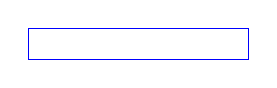
\begin{tikzpicture}[scale=.4]
  \draw[blue] (0,0) rectangle (7,1);
 \end{tikzpicture} representa $\dfrac{4}{5}$ de uma tira de papel, desenhe a tira completa.
 
 \item Investigue que tipo de frações geram dízimas finitas. Formule conjecturas e faça a prova.
 
 \item Observe a reta numérica onde estão marcados alguns números racionais representados pelas letras $A$, $B$, $C$ e $D$:
 
 \vspace{1cm}
 \begin{minipage}[h]{8cm}
 
 
     \begin{tikzpicture}[scale=5]

\draw[->] (-.3,0) -- (2.3,0);
\draw (0,.5pt) -- (0,-.5pt) node[anchor=north]{$0$};
\draw (1,.5pt) -- (1,-.5pt) node[anchor=north]{$1$};
\draw (2,.5pt) -- (2,-.5pt) node[anchor=north]{$2$};

\draw (1/3,.5pt) -- (1/3,-.5pt) node[anchor=north]{$A$};
\draw (5/6,.5pt) -- (5/6,-.5pt) node[anchor=north]{$B$};
\draw (1.5,.5pt) -- (1.5,-.5pt) node[anchor=north]{$C$};
\draw (2.05,.5pt) -- (2.05,-.5pt) node[anchor=north]{$D$};
\end{tikzpicture}
\end{minipage}
\vspace{1cm}

Qual a letra que melhor pode corresponder ao número que é o produto de $B$ por $C$? Marque na reta numérica o ponto que pode corresponder ao produto de $A$ por $C$. Marque também na reta numérica o ponto que pode corresponder à diferença entre $D$ e $C$.

\item Recorra às operações com frações para representar a parte sombreada da figura:

\begin{minipage}[h]{14cm}
\begin{center}
\begin{tikzpicture}[scale=1]
\draw (0,0) rectangle (4,2);
\draw (1,0) -- (1,2);
\draw (2,0) -- (2,2);
\draw (3,0) -- (3,2);

\draw (0,1) -- (1,1);

\draw[fill=grey!30] (0,1) rectangle (1,2);
\draw[fill=grey!30] (3,0) rectangle (4,8/7);

\draw (3,2/7) -- (4,2/7);
\draw (3,4/7) -- (4,4/7);
\draw (3,6/7) -- (4,6/7);
\draw (3,8/7) -- (4,8/7);
\draw (3,10/7) -- (4,10/7);
\draw (3,12/7) -- (4,12/7);
\end{tikzpicture}

\end{center}
\end{minipage}

\item Represente, recorrendo ao modelo de área, a seguinte expressão numérica:

$$\dfrac{1}{3}\times \dfrac{2}{5}+\dfrac{2}{3}\times \dfrac{1}{5}$$

\item Diga como procederia para calcular mentalmente os resultados das seguintes operações com números racionais:
\begin{multicols}{4}
\begin{enumerate}
    \item $2+\dfrac{1}{4}$
    \item $1-\dfrac{1}{4}$
    \item $3\times 3\dfrac{1}{5}$
    \item $3 \div \dfrac{1}{3}$
    \item $\dfrac{1}{2}+\dfrac{1}{4}$
    \item $\dfrac{1}{2}-\dfrac{1}{8}$
    \item $\dfrac{1}{2}\times \dfrac{3}{5}$
    \item $3\div\dfrac{3}{4}$
    \item $0,2+\dfrac{1}{5}$
    \item $0,5-\dfrac{1}{5}$
    \item $0,1\times \dfrac{1}{2}$
    \item $\dfrac{1}{3}\div 4$
    \item $\dfrac{2}{3}+5$
    \item $\dfrac{5}{3}-1$
    \item $\dfrac{3}{8}\times 8$
    \item $\dfrac{18}{16}\div\dfrac{9}{4}$
\end{enumerate}
\end{multicols}

Explique os raciocínios.

\section{Números Racionais em forma de Frações}

O conteúdo das frações é megaconceito pois engloba uma dezenas de outros. O seu trabalho desenvolve funções cognitivas que serão base para muitos outros conteúdos.

Algumas ideias chaves são:
\begin{enumerate}
    \item Uma fração pode ser maior que uma unidade;
    \item Duas frações podem ser equivalentes;
    \item Uma fração indica divisão em partes iguais;
    \item A fração conserva e recupera a unidade;
    \item Existe uma ordem entre as frações.
\end{enumerate}

Baseado em \cite{onuchic2008diferentes}, temos as seguintes personalidades dos números racionais:

\section{Ponto Racional}
Problemas que pedem para localizar números fracionários na reta numérica são ótimas oportunidades de trabalhar com essa personalidade. Todo número racional tem um ponto bem definido na reta e todo ponto racional da reta corresponde um número racional. 


\section{Quociente}
Essa personalidade normalmente é persebida quando um número de objetos precisa ser repartido igualmente num certo número de grupos. Esses objetos podem ter natureza contínua (pizza, barra) ou discreta (brinquedos).

Temos o dividendo e o divisor.A barra fracionária indica a função divisão. Essa personalidade é normalmente representado através da chave de divisão. Esse processo de aplica a diversos fenômenos como o processo de partição, extração, encolhimento e dedução.


\section{Fração}
Aqui temos a famosa relação parte-todo. Aqui interagem o numerador e o denominador. A barra fracionária apenas os separam.

Recomendo o jogo \textit{Loto }




\section{Operador}
Ocorre quando o múltiplicador (primeira parcela da multiplicação) é constituido por um número racinal. Por exemplo temos $\dfrac{3}{5}\times 15$.



Note que a barra fracionária indica a composição de operações divisão e multiplicação. 

Essa personalidade surge quando vamos encolher, esticar, reduzir ou ampliar algo.

\section{Razão}

Razão é uma comparação multiplicativa entre duas grandezas e não uma fração. Nelas se relacionam os termos antecedentes e consequêntes.

Essa personalidade é mais um conceito que liga diversos conteúdos como: regra de três, divisão em partes proporcionais, quantidades intensivas e extencivas, misturas, porcentagem, taxas, juros, descontos, escalas, estimativas populacionais, variação direta, variação inversa, razões trigonométricas, semelhança de triângulos, probabilidades, etc, além de ser base para o conceito de proporcionalidade.

\section{Proporcionalidade}
\end{enumerate}

%http://www.conhecer.org.br/enciclop/2015a/jogos%20matematicos.pdf

%http://arquivoabc.blogspot.com.br/p/fracoes.html
%http://www.sapientia.pucsp.br/tde_arquivos/3/TDE-2007-06-14T13:03:34Z-3492/Publico/dissertacao_wilson_roberto_rodrigues.pdf
%INCLUIR EXERCÍCIOS DOS COMPLEMENTOS E DO ARTIGO.

Livro: Física Conceitual
Capítulo: 12-Sólidos
Tópicos: Densidade (pg217), Mudanças de Escala (pg 223)

O que produz mais cascas, descascar 5kg de batatas grandes ou 5kg de batatas pequenas?

Área e volume não são diretamente proporcionais entre si.

\begin{enumerate}
    \item O que acontese ao volume de um pão que é esmagado? E à massa? E à densidade?
    \item O que é mais denso, algo que tenha uma densidade de $1.000 kg/m^3$, ou algo com densidade de $1g/cm^3$? Justifique sua resposta.
    \item O ósmio não é o átomo mais pesado encontrado na natureza. O que, então, explica que o ósmio seja a substância mais densa encontrada na Terra?
    \item O que tem maior densidade, uma pesada barra de ouro puro, ou um anel de ouro puro? Justifique sua resposta.
    \item A força do braço de uma pessoa depende do seu comprimento ou da área de sua seção transversal?
    \item Qual é o volume de um cubo de açucar com lado de 1 centímetro? Qual é a área da seção transversal desse cubo?
    \item O peso de uma pessoa depende mais do volume ou da área superficial da pele?
    \item Se as dimensões lineares de um certo objeto são dobradas, em quanto cresce sua área superficial? Em quanto cresce seu volume?
    \item Quando cresce o volume de um objeto, sua área superficial também cresce. Durante este crescimento, a razão dos metros quadrados para os metros cúbicos aumentam ou diminuem?
\end{enumerate}



%Números Racionais
%%%%%%%%%%%%%%%%%%%%%%%%%%%%%%%%%%%%%%%%%%%%%%%%%%%%
\chapter{Equações do Primeiro Grau}

\section{Método da Falsa Posição}

O método da falsa posição foi utilizado pelos povos antigos para resolver uma equações. No caso de equações do primeiro grau eles executavam um processo para conseguir encontrar. Vejamos um exemplo disso.

\subsubsection{Exemplo}\textit{A uma certa quantidade foram acrescentados a sua quarta parte. Obtêve-se por fim $15$ unidades. Que quantidade é essa?}

O primeiro passo é reescrever a frase em linguajar matemático. A quantidade desconhecida será representado por $x$. A quarta parte dessa quantidade será $\dfrac{x}{4}$. 
\begin{align}
    x+\dfrac{x}{4}&=15
\end{align}

Depois que foi reescrito escolhese um valor de $x$ que chamaremos de $x_0$ que será uma resposta temporária para o nosso problema. Tomemos a precaução de escolher um valor para facilitar as contas. Digamos que $x_0=4$.

\begin{align}
x_0+\frac{x_0}{4}&=x_1\\
    4+\frac{4}{4}&=4+1\\
    x_1&=5
\end{align}

Agora basta triplicar a expressão inteira.

\begin{align}
x+\frac{x}{4}&=15\\
3x_0 +\frac{3\times x_0}{4}&=3\times 5
\end{align}

Assim verificamos que o valor procurado é $x=4\times 3 = 12$.

Varifique para $x_0=8$ e depois $x_0=12$.

\section{Método da Tentativa e Erro}

Aqui iremos chutar valores para o número misterioso e registrar o resultado. Apartir do comportamento do resultado iremos rastrear a resposta.

Para exemplificar verifiquemos o seguinte problema envolvendo equação do primeiro grau.

\begin{exe}
Ao pagar três cafezinhos e um sorvete com uma nota de R\$10,00, João recebeu R\$1,20 de troco. Se o sorvete custa R\$1,60 a mais que cada cafezinho, qual é, em reais, o preço de um cafezinho?
\end{exe}

Apesar de podermos calcular o valor dessa questão atribuindo uma variável ao valor do café e equacionando os dados para obter o seu valor, iremos chutar o valor do café e então encontrarmos a resposta a partir dele.

\begin{table}[h]
\centering
\begin{tabular}{c|c |c}
   Preço do café  & Preço do sorvete & Valor da conta \\
   \hline
  $1,00$   & $2,60$  & $5,60$\\
  $1,10$   & $2,70$  & $6,00$\\
  $1,20$   & $2,80$  & $6,40$\\
  \hline
\end{tabular}
\end{table}

Note que almentando em 0,10 o valor do café teremos um aumento de 0,40 no valor da conta. Podemos então aumentar progressivamente até obtermos o valor da conta.

Nesse tipo de situação não é tão complicado equacionar a solução. Porém em provas que o objetivo não mede apenas a capacidade de resolução de problemas mas também a eficácia em um tempo curto, pensar em um método de resolver o problema de maneira mais rápida é essencial.

Recomendo que se siga as quatro etapas para a resolução de problemas conforme Polya:
\begin{enumerate}
\item Compreensão do problema: Para compreender um problema é necessário estimular o aluno a fazer perguntas:
\begin{itemize}
\item O que é
solicitado? 
\item Quais são os dados? Quais são as condições? 
\item É possível satisfazer as condições?
\item 
Elas são suficientes ou não para determinar a solução? Faltam dados? 
\item Que relações posso
estabelecer para encontrar os dados omitidos? 
\item Que fórmulas e/ou algoritmos posso utilizar?
\end{itemize}
Neste processo de compreensão do problema, muitas vezes torna-se necessário construir
figuras para esquematizar a situação proposta, destacando valores, correspondências e uso da
notação matemática.

\item Construção de uma estratégia de resolução: É importante estimular o aluno a buscar conexões entre os dados e o que é solicitado, estimulando, também, que pensem em situações similares, a fim de que possam estabelecer um plano de resolução, definindo prioridades e, se necessário, investigações complementares
para resolver o problema.

\item Execução de uma estratégia escolhida: Esta etapa é o momento de “colocar as mãos na massa”, de executar o plano idealizado. Se as etapas anteriores foram bem desenvolvidas, esta será, provavelmente a etapa mais fácil do processo de resolução de um problema. Para que o aluno obtenha sucesso, deve ser estimulado a realizar cada procedimento com muita atenção, estando atento a cada ação desenvolvida, verificando cada passo. O aluno também deve ser estimulado a mostrar que cada procedimento realizado está correto, possibilitando a afirmação de seu aprendizado e a comunicação de sua produção.

\item Revisão da solução: A revisão é um momento muito importante, pois propicia uma depuração e uma abstração da solução do problema. A depuração tem por objetivo verificar os procedimentos utilizados, procurando simplificá-los ou, buscar outras maneiras de resolver o problema de forma mais simples. A abstração tem por finalidade refletir sobre o processo realizado procurando descobrir a essência do problema e do método empregado para resolvê-lo, de modo a favorecer uma transposição do aprendizado adquirido neste trabalho para a resolução de
outras situações-problema.
\end{enumerate}





%Eq. prmeiro grau
%%%%%%%%%%%%%%%%%%%%%%%%%%%%%%%%%%%%%%%%%%%%%%%%%%%%
\chapter{Divisibilidade}
\section{Contextualizando Multiplos e Divisores com áreas}

Os múltiplos de um número podem ser compreendidos como áreas de retângulos cujo um dos lados é o número de quem estamos procurando os divisores e o outro são os valores por quem estamos mutiplicando para encontrar os múltiplos. Por exemplo, imaginem que estamos procurando os múltiplos de 7.  Basta desenhar um retângulo em que um lado é 7 e o outro lado varia entre os valores inteiros. Por exemplo.
\begin{figure}[h]
    \centering
    \begin{tikzpicture}
 \draw[blue] (0,0) rectangle (10,7);
%\foreach \x in {2,3,4,5,6,7,8,9,10,11,12,13}  {\draw[blue] (\x,1) -- (\x,7)}% \node [above] ($\x$) at (\x+.5,7);
\draw[blue] (1,0)--(1,7);
\node[above] (1) at (.5,7) {$1$};
%\draw[blue] (2,0)--(2,7);
\draw[blue] (3,0)--(3,7);
\node[above] (2) at (2,7) {$2$};
%\draw[blue] (4,0)--(4,7);
%\draw[blue] (5,0)--(5,7);
\draw[blue] (6,0)--(6,7);
\node[above] (3) at (4.5,7) {$3$};
%\draw[blue] (7,0)--(7,7);
%\draw[blue] (8,0)--(8,7);
%\draw[blue] (9,0)--(9,7);

\node[above] (4) at (8,7) {$4$};
 
\node [left] (A) at (0,3.5) {$7$}; %nó A
 \end{tikzpicture}
    \caption{Múltiplos e Áreas}
    \label{fig:my_label}
\end{figure}


A área do primeiro retângulo corrsponde ao produto do seu comprimento e de sua altura é $7$, o do segundo é $14$. Assim temos a sequência dos quatro primeiros múltiplos de 7.

Quais são esses múltiplos? Como posso obter os $10$ primeiros múltiplos de 7 combinando as áreas dos retângulos acima?

Façam a mesma coisa para achar $10$ primeiros múltiplos de $5,6,8$ e $9$;

\subsection{Múltiplos e Tabuada}

Notem que obter os múltiplos de um número equivale a fazer a sua tabuada. Note que a tabuada do $7$ é constituida dos $10$ primeiros múltiplos de $7$. A mesma coisa acontece para os $10$ primeiros múltiplos de $1, 2, 3, \dots$.

Como posso obter a tabuada de um número apartir do conceito de área como foi mostrado nesse caso para os múltiplos?

\section{Múltiplos e divisores}
\begin{multicols}{2}
Os números $0,1,2,3,$ etc. serão chamados aqui de números naturais. O conjunto dos números naturais será denotado por $\mathbb{N}$ e escreveremos $n\in \mathbb{N}$ para indicar que o número \textit{n} é um número natural.

Vamos começar observando algumas divisões.\\

\textbf{Exemplo 1}

\begin{center}
  %  \begin{tabular}{p{15mm}p{15mm}p{15mm}p{15mm}}
    \begin{tabular}{p{15mm} p{15mm} p{15mm} p{15mm}}
    \begin{array}{r|r} 14 & 5 \\ \cline{2-2} -10 & 2\\ \cline{1-1} 4 &  \end{array}     & \begin{array}{r|r} 12 & 3 \\ \cline{2-2} -12 & 4\\ \cline{1-1} 0 &  \end{array} & \begin{array}{r|r} 15 & 4 \\ \cline{2-2} -12 & 3\\ \cline{1-1} 3 &  \end{array} & \begin{array}{r|r} 18 & 6 \\ \cline{2-2} -18 & 3\\ \cline{1-1} 0 &  \end{array} \\
    \end{tabular}
\end{center}


\textit{Valem as seguintes relações para esses números:} $14=5\cdot 2+4$, $12=3\cdot 4 +0$, $15=4\cdot 3 +3$ \textit{e} $18=6\cdot 3 + 0$.

Em geral, em uma divisão, onde $b\not= 0$,

\[\begin{array}{c|c} a & b\\ \cline{2-2} r & q \end{array}\]

\textbf{Exemplo 2} Nas divisões do exemplo 1, os números 14, 12, 15 e 18 são os dividendos, os números 5,3,4 e 6 são os divisores e os números 2,4,3 e 3 são os quocientes e os números 4,0,3 e 0 são os restos das divisões.

Em duas das divisões do exemplo 1, o resto é igual a zero. Quando isso acontece, dizemos que a divisão é exata. Isso quer dizer, por exemplo, que a divisão de 12 por 3 e a divisão de 18 por 6 são exatas, porque os restos nessas divisões são iguais a zero, enquanto as outras duas divisões do exemplo 1 não são exatas, porque têm restos diferentes de zero.

\end{multicols}
%Divisibilidade
%%%%%%%%%%%%%%%%%%%%%%%%%%%%%%%%%%%%%%%%%%%%%%%%%
\chapter{Produtos Notáveis}

Produtos notáveis são multiplicações algébricas que ocorrem com frequência. 

\section{Quadrado da soma}

\begin{equation}
(a+b)^2=a^2+2ab+b^2
\end{equation}

\subsection{Justificativa Geométrica}
\begin{figure}[h]
    \centering
    \includegraphics[scale=1]{./imagens/12.png}
    \caption{Quadrado da Soma}
    \label{fig:my_label}
\end{figure}

\section{Quadrado da Diferença}

\begin{equation}
(a-b)^2=a^2-2ab+b^2
\end{equation}

\section{Produto da soma pela diferença}

\begin{equation}
(a+b)(a-b)=a^2+b^2
\end{equation}

\subsection{Justificativa Geométrica}
\begin{figure}[h]
    \centering
    \includegraphics[scale=.6]{./imagens/29.png}
    \caption{Produto da soma pela diferença}
    \label{fig:my_label}
\end{figure}

\section{Cubo da soma}

\begin{equation}
(a+b)^3=a^3+3a^2+3ab^2+b^3
\end{equation}

\subsection{Justificativa Geométrica}

\begin{figure}[h]
    \centering
    \includegraphics[scale=.5]{./imagens/13.png}
    \caption{Cubo da Soma}
    \label{fig:my_label}
\end{figure}

\section{Cubo da diferença}

\begin{equation}
(a-b)^3=a^3-3a^2+3ab^2-b^3
\end{equation}
%Produtos Notáveis
%%%%%%%%%%%%%%%%%%%%%%%%%%%%%%%%%%%%%%%%%%%%%%%%%%%
\chapter{Fatoração}

\section{Por em Evidência}

\begin{align}
    a+ab&=a(1+b)\\
    a^2b+ab^2&=ab(a+b)
\end{align}

\section{Agrupar}

\begin{align}
    ac+ad+bc+bd&=a(c+d)+b(c+d)\\
    &=(a+b)(c+d)\\
    2ac-2bc+4ad-bc&=2a(c+2d)-3bc
\end{align}

%\end{figure}%Fatoração
%%%%%%%%%%%%%%%%%%%%%%%%%%%%%%%%%%%%%%%%%%
\chapter{Função Modular}

O Módulo é uma entidade matemática conhecida por determinar o comprimento das coisas. Em se tratando do movimento teremos que o modulo corresponderia ao deslocamento de uma partícula P por uma distância percorrida.

Na Geometria Euclidiana Plana a figura que está totalmente entrelaçada com a ideia de distância é o círculo. Nele todos os pontos que estão em sua borda estão a mesma distância do seu sentro. É tanto assim que na Geometria Analítica a equação que define o círculo é definida pela distância entre os seus pontos e o seu centro.

\section{Distância entre dois pontos do Eixo Real}
\begin{center}
\begin{tikzpicture}
\draw[->] (-2,0) -- (2,0)
\end{tikzpicture}
\end{center}

\section{A distância e o círculo}
No plano a distância entre dois pontos é dado por $$d(A,B)=\sqrt{(x_A-x_B)^2+(y_A-y_B)^2}$$
de forma que os pontos tem a definição abaixo.
$$A=(x_A, y_A) \mbox{ e }B=(x_B, y_b)$$

Seja $C=(a,b)$ o centro de um círculo e \textit{r} o ráio desse círculo, temos que qualquer ponto $P=(x,y)$ sobre o círculo está a uma distância \textit{r} do centro. Ou seja:
\begin{align*}
 \sqrt{(x-a)^2+(y-b)^2}&=r\\
 (x-a)^2+(y-b)^2&=r^2
\end{align*}

Para entender bem essa fórmula basta pensar que a distância horizontal $(x_a)$ e a distância vertical $(y-b)$ são catetos de um triângulo retângulo em que \textit{r} é a hipotenúsa. Temos assim apenas uma simples aplicação do Teorema de Pitágoras.

\section{Distância em dimenções}

Note que se limitarmos o conceito de distância de um certo ponto ao plano (duas dimenções) teremos o círculo. O que ocorreria se colocassemos o mesmo conceito em um universo de três dimenções? Qual a figura geométria que tem a característica de ter todos os pontos de sua superfície a mesma distância do seu centro? Exatemente. A Esfera.

Na Geometria Analítica a esfera é definida de forma muito semelhante ao do círculo. A diferença é que no lugar de termos apenas duas coordenadas (x e y) teremos três (x, y e z).

Seja $O=(a,b,c)$ o centro da esfera, \textit{R} o seu raio e $P=(x,y,z)$ um ponto genérico sobre a esfera teremos:

\begin{align*}
 d(P,O)&=R\\
 \sqrt{(x-a)^2+(y-b)^2+(z-c)^2}&=R\\
 (x-a)^2+(y-b)^2+(z-c)^2&=R^2
\end{align*}

Para compreender essa fórmula basta imaginar que as diferenças nos eixos x,y e z são, respectivamente, os valores dos das dimensões de uma caixa. Dessa forma R corresponde a maior diagonal da caixa.

Note que a fórmula da esféra é extremamente semelhante ao do círculo. Acrescentamos apenas um termo, o $(z-c)^2$.

Isso não ocorre por acaso. Sempre que formos acrescentando uma nova dimenção iremos acrescentar um novo termo e teremos a respectiva equação da "esfera" naquela dimenção.

Equivale a dizer que o círculo é uma esféra em dimenção 2. Por que não dizer também que a esfera ser um círculo de dimensão 3.

Iremos tomar como referência hora o círculo, hora a esfera. Mas são equivalentes, com a diferença apenas da dimensão em que existem.

\section{Intersecções}

Note que se tomarmos a equação da esfera (3 dimensões) e a calcularmos no ponto em que $z=0$ teremos precisamente a equação do círculo. Isso significa que a intersecção entre uma esfera e um plano é um círculo. 

Como a esfera é a forma geométrica espacial cujos pontos estão todos a mesma distância de seu centro, então os pontos dessa esfera que estão em um mesmo plano também tem que estar a mesma distância de um ponto.Caso esse ponto seja o centro da esfera teremos o círculo máximo (equador).

\subsection{Intersecção entre duas esferas}
Note que a intersecção entre 

\subsection{Intersecção entre círculo e reta numérica}
Podemos então, belo bem da ciência, pegar o círculo (duas dimensões) e verificar qual o seu equivamente em apenas uma dimensão. Por que em uma dimensão? Ora, por que a reta real numérica tem apenas uma dimensão.%Teo. Pitagoras
%\chapter{Grandezas Diretamente e Inversamente Proporcionais}

COMPETÊNCIA DE ÁREA 4 - CONSTRUIR NOÇÕES DE VARIAÇÃO DE GRANDEZAS PARA A COMPREENSÃO DA REALIDADE E A SOLUÇÃO DE PROBLEMAS DO COTIDIANO

\paragraph{1. “Identificar a relação de dependência entre grandezas”}
Comentário do professor: Aqui é essencial que o candidato demonstre que sabe identificar uma fórmula que relacione grandezas distintas, como a força e aceleração ou o volume e a pressão, por exemplo. Geralmente, o Enem opta por relações pouco estudadas nas escolas, justamente para que o aluno consiga chegar às fórmulas por meio da interpretação dos textos que acompanham a questão. Outra característica comum é que elas apresentem uma constante de proporcionalidade em sua composição.

\paragraph{2. “Resolver situação-problema envolvendo a variação de grandezas, direta ou inversamente proporcionais”}
Comentário do professor: Essa habilidade se baseia na aplicação de regras de três, classificadas como direta, composta ou inversa. As grandezas diretamente e inversamente proporcionais permitem resoluções pelas regras de três simples. No entanto, quando há mais de três elementos envolvidos, usa-se a composta, que se resume em algumas regras de três simples. Para desenvolver um pouco melhor o conceito, confira um exemplo de exercício no qual se usaria a regra de três composta:

“Cinco operários constroem 20 metros de um muro, trabalhando 10 horas por dia em um período de 20 dias. Quantos operários serão necessários para construir 30 metros, trabalhando 6 horas por dia durante apenas 5 dias?”

\paragraph{3. “Analisar informações envolvendo a variação de grandezas como recurso para a construção de argumentação”}
Comentário do professor: As alternativas apresentam argumentos baseados nas variações de grandeza e, a partir deles, os alunos precisam encontrar a resposta esperada por meio das próprias alternativas, ou seja, realizará cálculos matemáticos para cada uma delas, buscando a que resolveria corretamente a situação-problema.

\paragraph{4. “Avaliar propostas de intervenção na realidade envolvendo variação de grandezas”}
Comentário do professor: Mais uma vez, o Enem investe para que o candidato chegue à resolução do exercício por meio da análise de qual a proposta mais adequada para uma situação problema criada. Aqui as alternativas ganham o foco da questão.%Grand. dire. inver. proporcionais

%ENSINO MÉDIO
%%www.matematiques.com.br

\chapter{Conjuntos Numéricos}

\section{Números Naturais}
A partir da necessidade de contar as civilizações desenvolveram métodos de registros de quantidades. O pastor de ovelhas tomava uma pedrinha para cada ovelha que saia para pastar. Para cada ovelha que retornava ele retirava uma pedrinha de um local e punha em outro, caso ainda tivessem pedrinhas significa que alguma ovelha não voutou. Até hoje chamamos o processo de raciocínio numérico de calcular, o que remonta aos calculos que eram aquelas pedras utilizaram.

Com o passar do tempo métodos mais eficientes de notação foram desenvolvidos baseados em sistemas de numeração diversos. O que temos hoje é o sistema decimal e seus símbolos evoluiram para os números que vemos hoje em dia.

A sua construção teórica é basicamente o conceito de que cada número tem um sucessor e que para encontrá-lo basta somar ``um'' a ele. Chamamos o maior de sucessor e o anterior de antesessor, e a ambos chamamos de consecutivos. Além disso o único número natural que não tem um antesessor é o zero.

\begin{center}
\fbox{$\mathbb{N}=\{1,2,3, \dots\}$}
\end{center}

\section{Números Inteiros}
Podemos dizer que este conjunto é composto pelos números naturais, o conjunto dos opostos dos números naturais e o zero. Este conjunto pode ser representado por:

$$\mathbb{Z}=\{\dots, -3 -2, -1, 0, 1,2 ,3 , \dots \}$$

\subsection{Principais subconjuntos dos Inteiros}

$\mathbb{Z}^*=\{\dots, -3 -2, -1, 1,2 ,3 , \dots \}$

$\mathbb{Z}_+=\{ 0, 1,2 ,3 , \dots \}$

$\mathbb{Z}_-=\{\dots, -3 -2, -1, 0 \}$

\subsection{Explorando a subtração}




\subsection{Explorando a divisão}
O Conjunto dos Números inteiros corresponde a uma generalização dos Naturais. 

Ele é completo na soma, pórém não é completo na Divisão. Temos que deixar um resto nos inteiros. Baseado nisso temos a teori a dos restos.

Seja um número inteiro positivo N e um divisor D, teremos como resultado um quociente Q e um resto R. De tal forma que podemos representar essa divisão por:

$$N=D\times Q+R$$

Tomemos um caso particular. Costrua uma tabela em que a primeira coluna corresponde ao número N que está sendo dividido, a segunda a quantidade de parcelas (o quociente) e a terceira o resto.

\begin{table}[h]
 \centering
 \begin{tabular}{|c|c|c|c|c|}
 \hline
 Valor & Parcelas & Resto & Notação\\
 \hline
 0 & 0 & 0 & $0=0\times 3 + 0$\\
 \hline
 1 & 0 & 1 & $1=0\times 3 + 1$\\
 \hline
 2 & 0 & 2 & $2=0\times 3 + 2$\\
 \hline
 3 & 1 & 0 & $3=1\times 3 + 0$ \\
 \hline
 4 & 1 & 1 & $4=1\times 3 + 1$\\
 \hline
 5 & 1 & 2 & $5=1\times 3 + 2$\\
 \hline
 6 & 2 & 0 & $6=2\times 3 + 0$\\
 \hline
 7 & 2 & 1 & $7=2\times 3 + 1$\\
 \hline
 8 & 2 & 2 & $8=2\times 3 + 2$\\
 \hline
 \end{tabular}
 \caption{Tabela dos restos na divisão por 3}
 \label{tab:my_label}
\end{table}

Peça para os alunos continuar a tabela até o número 18. Explore os padrões.
Algumas atividades interessantes para serem feitas baseadas nessa tabela:
\newpage
\begin{enumerate}

 \item Você identificou algum padrão nos restos?
 \item Quem são os números que restam 0? O que eles tem em comum com a tabuada de 3?
 \item Quem são os números que restam 1? Qual a relação que ele tem com os múltiplos de 3?
 \item Quem são os números que restam 2? Qual a sua relação com os múltiplos de 3?
\end{enumerate}

\section{Números Racionais}

\section{Números Reais}


\section{Resumo}

\subsection{O conjunto dos números naturais N}

O mais simples. Por ser um conjunto discreto, pode ter uma representação explícita:

$\mathbb{N} = \{0, 1, 2, 3, 4, 5 \dots\}$
 
\subsection{O conjunto dos números inteiros Z}

É o que resulta da expansão de $\mathbb{N}$ na integração dos números negativos. Por ser um conjunto discreto, pode ter representação explícita: $\mathbb{Z} = \{\dots,-3, -2, -1, 0, 1, 2, 3,\dots\}.$
 
\subsection{O conjunto dos números racionais Q}

É a expansão do conjunto $\mathbb{Z}$, na qual o campo numérico passa a ocupar a parte racional da continuidade.

Por não ocupá-la completamente, é considerado um conjunto denso, sem representação explícita. 
Pode existir na reta, desde que se indiquem os espaços vazios da descontinuidade, que correspondem aos números irracionais, também à esquerda de zero.

Proponha o seguinte jogo: dois alunos tentam falar cada um um número que seja maior que o outro dentro dos números naturais. Depois fazem o mesmo mas com um limite superior aberto e depois fechado. Depois fazem a mesma coisa só que nos racionais, primeiro com limite superior fechado e depois aberto. O objetivo é que vejam que é sempre possível escolher um número maior nos racionais que não ultrapasse um certo limite aberto. 
 
\subsection{O conjunto dos números reais R}

É a expansão do conjunto $\mathbb{Q}$ na qual o campo numérico passa a ocupar toda a continuidade, graças à união dos campos racional e irracional. Por se tratar de um conjunto contínuo, não tem representação explícita. É um conjunto numérico que ocupa todos os pontos da reta, também à esquerda de zero.

%%%%%%%%%%%%%%%%%%%%%%%%%%%%%%%%%%%%%%%%%%%%
%Conjuntos numéricos
%\chapter{Revisão}
\section{Operações}
A adição é uma das primeiras operações que aprendemos. Ela normalmente trás a ideia de união de quantidades. Mas devemos ter cuidado que a adição também pode vir mascarada de outras fórmas como a ideia de ``falta'', normalmente associada a subtração.

A soma é uma operação que tem propriedades tais como a associação, comutatividade, neutro e simétrico.

\section{Frações}

\section{Razões, Proporções e Porcentagem}

\section{Potenciação e Radiciação}

\subsection{Potencia de expoente Natural}
\begin{center}
\fbox{$ a^n=a \cdot a \cdot \dots a$}
\end{center}

\textit{n} é o expoente e \textit{a} é a base.

Exemplos
\begin{align*}
3^3&=\\
2^4&=\\
(-3)^3&=\\
(-3)^4&=
\end{align*}

O que ocorre quando o expoente é par? E quando é impar?
\begin{center}

\fbox{\begin{cases}
a^0=1 \\ a^1=a
\end{cases}}

\end{center}

\subsubsection{Propriedades}

\begin{tabular}{lrl}

 P1 & $a^n \cdot a^m=$ &$a^{n+m}$ \\

 P2 & $\dfrac{a^m}{a^n}=$ &$a^{m-n}$\\

 P3 & $(a^m)^n=$&$a^{m\cdot n}$ \\

 P4 & $ (a \cdot b)^m =$&$a^m \cdot b^m $ \\

 P5 & $ \left( \dfrac{a}{b} \right )^m =$&$ \dfrac{a^m}{b^m}$\\

\end{tabular}
\\\\\\\\
Exemplo:
\begin{align*}
 3^3 \cdot 3^2&=\\
 \dfrac{2^4}{2^3}&=\\
 (4 \cdot 3)^3&=\\
 (4^2)^2&=\\
 \left( \dfrac{2}{3} \right)^2&=\\
 (5^4 \cdot 5^6)\div 5^{10}&=\\
 \dfrac{2^{x+5}}{2^x}-\dfrac{2^{x-2}}{2^x}&=
\end{align*}

\subsubsection{Potência de Expoente Inteiro Negativo}

OBSERVAÇÃO: Inverter a base e trocar o expoente do sinal do expoente. Ou seja:
\begin{center}
\fbox{ $a^{-n}=\left(\dfrac{1}{a} \right)^n$}
\end{center}

Exemplos:
\begin{align*}
 2^{-3}&=\\
 4^{-2}&=\\
 \left(\dfrac{1}{4} \right)^{-3}&=\\
 \sqrt{3}^{-2}&=\\
\end{align*}

\subsubsection{Potência de Expoente Racional}


\begin{center}
\fbox{$\sqrt[n]{a^m}=a^{\frac{m}{n}}$}
\end{center}

Exemplos:

\begin{align*}
 \sqrt[5]{128}&=\\
 \sqrt{1024}&=\\
\end{align*}

Propriedades:

\begin{tabular}{lrl}

 P1 & $\sqrt[n]{a} \cdot \sqrt[n]{b}=$ &$\sqrt[n]{ab}$ \\

 P2 & $(\sqrt[n]{a^m})^p=$ & $\sqrt[n]{a^{mp}}$\\

 P3 & $\sqrt[x]{\sqrt[y]{a}}=$ & $\sqrt[xy]{a}$ \\

\end{tabular}

\subsubsection{Equações Exponenciais}

Exemplo
\begin{equation}
 5^x-5^{2-x}=24\\
\end{equation}

\begin{itemize}
 \item Gráfico
 \item Estudo de sinal
 \item Base diferente de zero, diferente de um, positiva
 \item Estudo de dois casos, base entre zero e um e base maior que um
 \item Estudo do gráfico de $f(x)=2^{ax+b}+c$ quando se varia a, b e c um por vez.
\end{itemize}

%Revisão
%\chapter{Intervalos}

Os intervalos são basicamente subconjunto dos números reais. Como os números reais são densos, ou seja, entre dois números reais sempre existe um outro número real, logo entre os números 2 e 3 existem infinitos números reais. 

Os intervalos podem ser dos seguintes tipos:

\begin{figure}[h]
 \centering
\begin{tikzpicture}[scale=4]
\draw (-1,0) -- (1,0);
\coordinate[label=below:$a$] (A) at (-.5,0);
\coordinate[label=below:$b$] (B) at (.5,0);
\draw[blue, thick] (A) -- (B);
\filldraw[blue] (A) circle (.5pt) node[anchor=west];
\filldraw[blue] (B) circle (.5pt) node[anchor=west];
\filldraw[white] (A) circle (.48pt) node[anchor=west];
\filldraw[white] (B) circle (.48pt) node[anchor=west];
\end{tikzpicture}
\caption{Intervalo aberto: $a<x<b$}
 \label{fig:my_label}
\end{figure}

\begin{figure}[h]
 \centering
\begin{tikzpicture}[scale=4]
\draw (-1,0) -- (1,0);
\coordinate[label=below:$a$] (A) at (-.5,0);
\coordinate[label=below:$b$] (B) at (.5,0);
\draw[blue, thick] (A) -- (B);
\filldraw[blue] (A) circle (.5pt) node[anchor=west];
\filldraw[blue] (B) circle (.5pt) node[anchor=west];
\end{tikzpicture}
 \caption{Intervalo fechado: $a\leq x \leq b$}
 \label{fig:my_label}
\end{figure}

\begin{figure}[h]
 \centering
\begin{tikzpicture}[scale=4]
\draw (-1,0) -- (1,0);
\coordinate[label=below:$a$] (A) at (-.5,0);
%\coordinate[label=below:$b$] (B) at (.5,0);
\draw[blue, thick] (A) -- (1,0);
\filldraw[blue] (A) circle (.5pt) node[anchor=west];
%\filldraw[blue] (B) circle (.5pt) node[anchor=west];
\filldraw[white] (A) circle (.48pt) node[anchor=west];
%\filldraw[white] (B) circle (.48pt) node[anchor=west];
\end{tikzpicture}
\caption{Intervalo aberto: $a<x$}
 \label{fig:my_label}
\end{figure}

\begin{figure}[h]
 \centering
\begin{tikzpicture}[scale=4]
\draw (-1,0) -- (1,0);
\coordinate[label=below:$a$] (A) at (-.5,0);
\coordinate[label=below:$b$] (B) at (.5,0);
\draw[blue, thick] (A) -- (B);
\filldraw[blue] (A) circle (.5pt) node[anchor=west];
\filldraw[blue] (B) circle (.5pt) node[anchor=west];
\end{tikzpicture}
 \caption{Intervalo fechado: $a\leq x \leq b$}
 \label{fig:my_label}
\end{figure}

%Intervalos
%%%%%%%%%%%%%%%%%%%%%%%%%%%%%%%%%%%%%%%%%%%%%%%%%%%%%%%%
\chapter{Progressão Aritmética}
Como as progressões Aritméticas são ótimas para a introdução do conceito de função afim e quadrática o curso de Progressões foi desmembrado em duas partes. A primeira apenas de Progressão aritmética para ser apresentado antes de função afim. E depois o de Progressão geométrica antes de função exponencial.
%http://www.somaticaeducar.com.br/arquivo/material/112008-08-23-19-28-11.pdf

\begin{itemize}
 \item Regra de formação;
 \item Razão;
 \item Termo geral;
 \item Soma de termos;
\end{itemize}

\section{Juros símples}

%Progressão Aritmética
%%%%%%%%%%%%%%%%%%%%%%%%%%%%%%%%%%%%%%%%%%%%%%%%%%%%%%%%
\chapter{Função Afim}
%http://www.unifal-mg.edu.br/matematica/?q=pifc-funcao-progressao
Vamos relembrar a tabuada de 3.


\begin{table}[h]
\begin{center}
 \begin{tabular}{|c|c|c|c|c|c|c|c|c|c|}
 \hline
 1 & 2 & 3 & 4 & 5 & 6 & 7 & 8 & 9 & 10 \\
 \hline
 & & & & & & & & & \\
 \hline
 \end{tabular}
 \end{center}
 \caption{Múltimos de 3}
 \label{tab:my_label}
\end{table}

Coloque os números de 1 a 10 sobre um eixo horizontal das abcissas e os valores encontrados sobre o eixo das ordenadas. Trace os pontos e depois a reta. Faça outra tabela e repita o processo para os múltiplos de outros valores como 2, 4 e 5.

\begin{itemize}
 \item Relação com Progressão Aritmética
 \item Tabela Entrada e Saída
 \item Pontos no Plano Cartesiano
 \item Gráfico é uma Reta
 \item Coeficiente Ângular e Linear
 \item Domínio e Imagem
 \item Equação da Reta
 \item Zeros da Função
 \item Estudo de Sinal
\end{itemize}


%Função Afim
%%%%%%%%%%%%%%%%%%%%%%%%%%%%%%%%%%%%%%%%%%%%%%%%%%%%%%%%
\chapter{Função Quadrática}



\begin{itemize}
 \item Mostrar que as funções quadráticas tem uma progressão aritmética de segunda ordem imbutida
 \item Gráfico
 \item Estudo da concavidade
 \item Estudo dos sinais da função
\end{itemize}

\begin{center}
\includegraphics[scale=.5]{./imagens/25.png}
\includegraphics[scale=1]{./imagens/30.png}
\end{center}


%Função Quadrática
%%%%%%%%%%%%%%%%%%%%%%%%%%%%%%%%%%%%%%%%%%%%%%%%%%%
\chapter{Fatoração}

\section{Por em Evidência}

\begin{align}
    a+ab&=a(1+b)\\
    a^2b+ab^2&=ab(a+b)
\end{align}

\section{Agrupar}

\begin{align}
    ac+ad+bc+bd&=a(c+d)+b(c+d)\\
    &=(a+b)(c+d)\\
    2ac-2bc+4ad-bc&=2a(c+2d)-3bc
\end{align}

%\end{figure}%Inequações
%%%%%%%%%%%%%%%%%%%%%%%%%%%%%%%%%%%%%%%%%%
\chapter{Função Modular}

O Módulo é uma entidade matemática conhecida por determinar o comprimento das coisas. Em se tratando do movimento teremos que o modulo corresponderia ao deslocamento de uma partícula P por uma distância percorrida.

Na Geometria Euclidiana Plana a figura que está totalmente entrelaçada com a ideia de distância é o círculo. Nele todos os pontos que estão em sua borda estão a mesma distância do seu sentro. É tanto assim que na Geometria Analítica a equação que define o círculo é definida pela distância entre os seus pontos e o seu centro.

\section{Distância entre dois pontos do Eixo Real}
\begin{center}
\begin{tikzpicture}
\draw[->] (-2,0) -- (2,0)
\end{tikzpicture}
\end{center}

\section{A distância e o círculo}
No plano a distância entre dois pontos é dado por $$d(A,B)=\sqrt{(x_A-x_B)^2+(y_A-y_B)^2}$$
de forma que os pontos tem a definição abaixo.
$$A=(x_A, y_A) \mbox{ e }B=(x_B, y_b)$$

Seja $C=(a,b)$ o centro de um círculo e \textit{r} o ráio desse círculo, temos que qualquer ponto $P=(x,y)$ sobre o círculo está a uma distância \textit{r} do centro. Ou seja:
\begin{align*}
 \sqrt{(x-a)^2+(y-b)^2}&=r\\
 (x-a)^2+(y-b)^2&=r^2
\end{align*}

Para entender bem essa fórmula basta pensar que a distância horizontal $(x_a)$ e a distância vertical $(y-b)$ são catetos de um triângulo retângulo em que \textit{r} é a hipotenúsa. Temos assim apenas uma simples aplicação do Teorema de Pitágoras.

\section{Distância em dimenções}

Note que se limitarmos o conceito de distância de um certo ponto ao plano (duas dimenções) teremos o círculo. O que ocorreria se colocassemos o mesmo conceito em um universo de três dimenções? Qual a figura geométria que tem a característica de ter todos os pontos de sua superfície a mesma distância do seu centro? Exatemente. A Esfera.

Na Geometria Analítica a esfera é definida de forma muito semelhante ao do círculo. A diferença é que no lugar de termos apenas duas coordenadas (x e y) teremos três (x, y e z).

Seja $O=(a,b,c)$ o centro da esfera, \textit{R} o seu raio e $P=(x,y,z)$ um ponto genérico sobre a esfera teremos:

\begin{align*}
 d(P,O)&=R\\
 \sqrt{(x-a)^2+(y-b)^2+(z-c)^2}&=R\\
 (x-a)^2+(y-b)^2+(z-c)^2&=R^2
\end{align*}

Para compreender essa fórmula basta imaginar que as diferenças nos eixos x,y e z são, respectivamente, os valores dos das dimensões de uma caixa. Dessa forma R corresponde a maior diagonal da caixa.

Note que a fórmula da esféra é extremamente semelhante ao do círculo. Acrescentamos apenas um termo, o $(z-c)^2$.

Isso não ocorre por acaso. Sempre que formos acrescentando uma nova dimenção iremos acrescentar um novo termo e teremos a respectiva equação da "esfera" naquela dimenção.

Equivale a dizer que o círculo é uma esféra em dimenção 2. Por que não dizer também que a esfera ser um círculo de dimensão 3.

Iremos tomar como referência hora o círculo, hora a esfera. Mas são equivalentes, com a diferença apenas da dimensão em que existem.

\section{Intersecções}

Note que se tomarmos a equação da esfera (3 dimensões) e a calcularmos no ponto em que $z=0$ teremos precisamente a equação do círculo. Isso significa que a intersecção entre uma esfera e um plano é um círculo. 

Como a esfera é a forma geométrica espacial cujos pontos estão todos a mesma distância de seu centro, então os pontos dessa esfera que estão em um mesmo plano também tem que estar a mesma distância de um ponto.Caso esse ponto seja o centro da esfera teremos o círculo máximo (equador).

\subsection{Intersecção entre duas esferas}
Note que a intersecção entre 

\subsection{Intersecção entre círculo e reta numérica}
Podemos então, belo bem da ciência, pegar o círculo (duas dimensões) e verificar qual o seu equivamente em apenas uma dimensão. Por que em uma dimensão? Ora, por que a reta real numérica tem apenas uma dimensão.%Função Modular
%\chapter{Revisão de Geometria}%Revisão de Geometria
%%%%%%%%%%%%%%%%%%%%%%%%%%%%%%%%%%%%%%%%%%%%%%%%%%
\chapter{Logarítmos}

%http://www.ime.unicamp.br/~chico/ma091/ma091_2014_34_manipulacao_de_logaritmos.pdf
Enquanto a função exponencial trabalha com o resultado das potências os logaritmos trabalha no plano dos expoentes. Nisso devemos anteriormente lembrar das propriedades de produto de potências, divisões e as outras pois terão respaldo nos logaritmos.

\section{Definição}
\section{Condições de Existência de um Logaritmo}
\section{Propriedades do logaritmo}

A função logaritma é a função inversa da função exponencial. Logo é natural deduzir as propriedades e leis de construção dos logaritmos apartir dos expoentes. 

\subsection{$\log_a (1)=0$}

Esse logaritmo é o caso geral da função $f(x)=a^0$. Temos aqui uma das propriedades de potências. Para todo valor de \textit{a} o valor de $f(0)=a^0=1$. Devemos ressaltar que o termo para $a=0$ é considerada uma indeterminação matemática.

\subsection{$\log_a (a)=1$}

Aqui temos a situação quando $x=1$, ou seja $f(1)=a^1=a$.

\subsection{$\log_a (a^x)=x$}

Da definição de logaritmo temos essa propriedade. Note que se tomarmos o caso anterior basta substituir o 1 por 2 e verifiar o resultado. Depois por três. Generalizando teremos o mesmo para um x qualquer.

\subsection{$a^{\log_a (a^x)}=x$}

Neste caso basta chamar o valor de $\log_a (x)=y$. Substituindo teremos que $a^y$. Ora, pela definição de logaritmos e pela substituição que fizemos temos que $a^y=x$. Outra maneira é fazer a substituição $x=a^y$. Utilizando a propriedade anterior poderemos confirmar a afirmação. Note que as duas substituições são equivalentes já que $\log_a (x)=y \Longleftrightarrow x=a^y$.

\section{Operações com Logaritmos}

\subsection{$\log_a (xy)=\log_a (x)+\log_a (y)$}

Essa operação conhecida como ``O produto dos logaritmandos corresponde a soma dos logaritmos'' é o motivo pelo qual os logaritmos foram criados. Essa propriedade transforma o produto de números grandes em soma de potênias. Em uma época antes da invenção de computadores com capacidade de fazerem cálculos instantaneamente como as calculadoras que cabem em nossos bolsos atualmente era o que possibilitava encontrar os resultados para problemas maritmos, astronômicos e econômicos.

Note que a propriedade do produto de potências de mesma base se equivale a essa regra. Lembre-se de observar os expoentes.

\subsection{$\log_a (\frac{x}{y})=\log_a (x)-\log_a (y)$}

\subsection{$\log_a (x^c)=c\log_a (x)$}

%Logaritmos
%\chapter{Progressão Geométrica}
\begin{itemize}
 \item Regra de formação;
 \item Razão;
 \item Termo geral;
 \item Soma de termos;
\end{itemize}

\section{Juros Compostos}%Progressão Geométrica
%%%%%%%%%%%%%%%%%%%%%%%%%%%%%%%%%%%%%%%%%%%%%%%%%%%%%%%%%
\chapter{Função Exponencial}
%http://repositorio.utfpr.edu.br/jspui/bitstream/1/832/1/CT_PROFMAT_M_Ferri%2c%20Orlando%20Eduardo%20da%20Silva_2014.pdf

%\begin{multicols}{2}



Função exponencial é uma ferramente matemática presente na descrição e análise de muitos fenômenos da vida real, tais como cálculos financeiros, datação de materiais arqueológicos por meio de técnicas que utilizam a radioatividade, estudo do crescimento ou decrescimento de uma população etc.

%\end{multicols%Função Exponencial
%%%%%%%%%%%%%%%%%%%%%%%%%%%%%%%%%%%%%%%%%%%%%%%%%%%%
\chapter{Trigonometria}

A trigonometria não é a ciência que mede os grãos de trigo, mas sim a ciência das sombras e das estrelas. Suas origens remontam a astronomia, agrimessura e as navegações.

Para Euclides (em sua obra chamada Elementos) foi dito que um ponto é algo que não tem dimensão ou parte alguma. A linha (em específico a reta) tem uma origem e uma extremidade que são pontos. A superfície corresponde corresponde a figura delimitada por linhas em sua borda. O plano é uma superfície que contem duas retas paralelas (ou concorrentes).

O círculo é uma figura interessante pois corresponde a superfície cujo todos os pontos de sua borda estão a mesma distância do seu centro. Além disso as linhas que ligam quaisquer dois pontos da borda do círculo é chamado de corda. A maior corda é a que passa pelo centro do círculo, ela é chamada de diametro do círculo. A metade do diametro é o raio.

\section{Contexto histórico}

O termo trigonometria significa a medida das partes de um triângulo.

Na grécia antiga temos estenços estudos entre os angulos (ou arcos) e as cordas em um mesmo círculo.

Hiparco foi chamado pai da trigonometria por ter desenvolvido cálculos precisos e com eles calcular a duração precisa do mês e do ano, o tamanho da luna e a precessão dos equinócios.

\section{Origem do termo seno}

Os árabes haviam traduzido textos de trigonometria do sânscrito. Os hindus tinham dado o nome de \textit{jiva} à metade da corda, e os árabes a transformaram em \textit{jiba}. Na língua árabe é comum escrever apenas as consoantes de uma palavra, deixando que o leitor acrescente mentalmente as vogais. Desse modo, os tradutores árabes registraram \textit{jb}. Na sua tradução do árabe para o latim, Robert de Chester interpretou \textit{jb} como as consoantes da palavra \textit{jaib}, que significa \textit{"baía"} ou \textit{"enseada"}, e escreveu \textit{sinus}, que é o equivalente em latim.\cite{eli1998trigonometric} e \cite{da2003historia} A partir daí, a \textit{jiba}, ou meia corda hindu passou a ser chamada de \textit{sinus}, e, em português, \textit{seno}.\footnote{\href{http://ecalculo.if.usp.br/historia/historia_trigonometria.htm}{Usp, Trigonometria}}

Uma das tarefas da astronomia foi o estabelecimento das tabelas. As primeiras tabelas, as de Hiparco, se perderam. Quanto às de Ptolomeu, estabeleciam as coorrespondências entre os comprimentos das cordas e dos diferentes valores de arcos.

Mais tarde os indianos substituíram as tabelas de cordas por tabelas de senos, mais fáceis manejar.


\begin{center}
\includegraphics[scale=0.9]{./imagens/06.png}
\end{center}

\begin{center}
\includegraphics[scale=0.9]{./imagens/07.png}
\end{center}

A precisão de todo cálculo astronômico repousa na exatidão da tabela de senos, cuja construção está ligada ao problema da trisseção do ângulo! Al-Khuwarizmi foi o primeiro matemático árabe a estabelecer tabelas de senos! \cite{guedj2008teorema}

%\begin{center}
%\includegraphics[scale=0.9]{8.png}
%\end{center}
\section{Trigonometria no Triangulo Retângulo}

\begin{center}
%\scalebox{2}{
\begin{tikzpicture}
\coordinate[label=below left:$A$] (A) at (0,0);
\coordinate[label=below right:$B$] (B) at (4,0);
\coordinate[label=above right:$C$] (C) at (4,3);
\coordinate[label=below :cateto adjacente] () at (4/2,0);

\draw[thick] (B) -- (A) -- (C) -- (B);

\begin{scope}
\path[clip] (A) -- (B) -- (C);
\end{scope}

\draw[->] (0,0) ++(.5,0) arc (0:35:.5);
\draw[] (4,0) rectangle (3.5,0.5);

\node at (35/2:.8) {$\theta$};
\node[above,left] at (4/2,3/2) {hipotenusa};
\node[right] at (4,3/2) {cateto oposto}
%\node[above] at (4/2,0) {cateto adjacente}

\end{tikzpicture}
%}
\end{center}

\begin{table}[h]
 \centering
 \begin{tabular}{|c|c|}
 \hline
 seno & cosseno \\
 \hline
 $\sin \theta=\dfrac{C. op}{Hip}=\dfrac{a}{b}$ & $\cos \theta=\dfrac{C. ad}{Hip}=\dfrac{c}{b}$\\
 \hline
 \end{tabular}
 \caption{Seno e Cosseno no triângulo retângulo}
 \label{tab:my_label}
\end{table}


\section{Ângulo complementar e o Cosseno}
Dois ângulos são complementares quando sua soma dão um ângulo reto.

\begin{table}[h]
 \centering
 \begin{tabular}{|c|c|}
 \hline
 ângulo & complementar \\
 \hline
 0° & 90°\\
 \hline
 30° & 60°\\
 \hline
 45° & 45°\\
 \hline
 60° & 30°\\
 \hline
 90° & 0°\\
 \hline
 \theta & $90°-\theta$\\
 \hline
 \end{tabular}
 \caption{Ângulos complementares somados resutam um ângulo reto}
 \label{tab:my_label}
\end{table}

O cosseno é o seno do ângulo complementar. Ou seja, o cosseno de um ângulo é o seno do quanto falta para que esse ângulo se torne um ângulo reto.

\begin{table}[]
 \centering
 \begin{tabular}{|c|c|}
 \hline
 cosseno & seno \\
 \hline
 $\cos 0°$ & $\sin 90°$\\
 \hline
 $\cos 30°$ & $\sin 60°$\\
 \hline
 $\cos 45°$ & $\sin 45°$\\
 \hline
 $\cos 60°$ & $\sin 30°$\\
 \hline
 $ \cos 90°$ & $\sin 0°$\\
 \hline
 $\cos \theta$ & $\sin (90-\theta)$\\
 \hline
 \end{tabular}
 \caption{O Cosseno de um ângulo é o seno de seu complementar}
 \label{tab:my_label}
\end{table}
\newpage

\section{Ângulos Notáveis}
Os triângulos notáveis com que trabalhamos no Ensino Fundamental são $30^o, 45^o$ e $60^o$. No triângulo equilátero obteremos o seno e o cosseno de dois desses valores e com o quadrado de diagonal unitária o outro valor.

\subsection{$30^o$ e $60^o$}
É sabido que na Geomtria Euclidiana Plana o triângulo tem ao todo $180^o$ de ângulo interno. Em um triângulo equilátero temos, assim, três ângulos medindo $60^o$.
\begin{center}
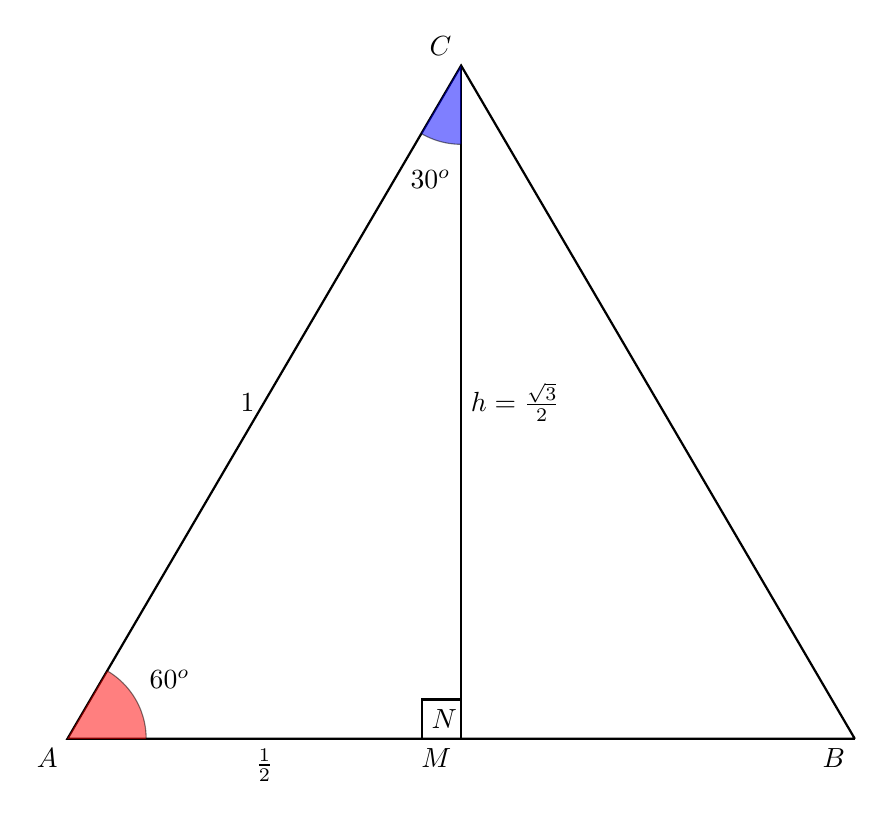
\begin{tikzpicture}[scale=5]

\coordinate [label=below left:$A$] (A) at (0,0);
\coordinate [label=below left:$B$] (B) at (2,0);
\coordinate [label=above left:$C$] (C) at (1,1.71);
\coordinate [label=below left:$M$] (M) at (1,0);
\coordinate [label=below right:$N$] (N) at (0.9,0.1);
%\coordinate [label=below right:$h=\sqrt{3}/2$] (O) at (1,1.71/2);

\draw[thick] (B) -- (A) -- (C) -- (B);
\draw[thick] (C) -- (M);
\draw[thick] (M) rectangle (N);

\begin{scope}
\path[clip] (A) -- (B) -- (C);
\fill[red, opacity=0.5, draw=black] (A) circle (2mm);
\node at ($(A)+(30:3mm)$) {$60^o$};

\path[clip] (C) -- (A) -- (M);
\fill[blue, opacity=0.5, draw=black] (C) circle (2mm);
\node at ($(C)+(255:3mm)$) {$30^o$};
\end{scope}

\node[right] at (1,1.71/2) {$h=\frac{\sqrt{3}}{2}$};
\node[left] at (1/2,1.71/2) {$1$};
\node[below] at (1/2,0) {$\frac{1}{2}$};

\end{tikzpicture}
\end{center}
\section{Relação Fundamental da Trigonometria}

A relação fundamental da Trigonometria afirma que

\begin{equation}
    \sin^2 (\theta)+\cos^2 (\theta)=1
\end{equation}.

Isso é facilmente verificável para o triângulo retângulo cuja hipotenusa mede uma unidade como na imagem abaixo.

\begin{figure}[h]
    \centering
\scalebox{1}{
\begin{tikzpicture}[scale=1.00]
\coordinate[label=below left:$A$] (A) at (0,0);
\coordinate[label=below right:$B$] (B) at (4,0);
\coordinate[label=above right:$C$] (C) at (4,3);
\coordinate[label=below :$\cos (\theta)$] () at (4/2,0);

\draw[thick] (B) -- (A) -- (C) -- (B);

\begin{scope}
\path[clip] (A) -- (B) -- (C);
\end{scope}

\draw[->] (0,0) ++(.5,0) arc (0:35:.5);
\draw[] (4,0) rectangle (3.5,0.5);

\node at (35/2:.8) {$\theta$};
\node[above] at (4/2,3/2) {$1$};
\node[right] at (4,3/2) {$\sin (\theta)$}
%\node[above] at (4/2,0) {$\cos (\theta)$}

\end{tikzpicture}
}
    \caption{Triângulo Retângulo de hipotenusa medindo uma unidade}
    \label{fig:my_label}
\end{figure}



\begin{figure}[h]
    \centering
    \includegraphics[scale=0.6]{./imagens/11.png}
    \caption{Círculo Trigonométrico de raio 1}
    \label{fig:my_label}
\end{figure}

\section{Seno e Cosseno da soma de arcos}



\section{Decomposição de Forças}

\begin{center}%Colocar alfa teta no lugar de alfa
\includegraphics[scale=0.9]{./imagens/10.png}
\end{center}\\



$F=(F_x,F_y)=(F\cos \theta,F\sin \theta)$

%Trigonometria
%%%%%%%%%%%%%%%%%%%%%%%%%%%%%%%%%%%%%%%%%%
\chapter{Física 1}
%http://sites.ifi.unicamp.br/f128/aulas/
%http://sites.ifi.unicamp.br/f128/ementa/
\section{Fórmulas Matemáticas}

\subsection{Movimento Retilíneo}

\begin{equation}\label{14.1}
    s=s_0+vt
\end{equation}

\subsection{Vetores}

O que é uma grandeza escalar?

Uma grandeza escalar é somente magniture; ela é apenas o número, positivo ou negativo.

O que é uma grandeza vetorial?

Uma grandeza vetorial é a junção de magniture com direção. Por exemplo, um cor se move para a direção sul a 40 km/h tem uma velocidade vetorial de 40km/h apontando para o sul.

SOMA VETORIAL

DESCRIÇÃO DE FUNÇÕES TRIGONOMÉTRICAS NO TRIÂGULO RETÂNGULO

COMPONENTES RETANGULARES DE UM VETOR.

ADIÇÃO DE VETORES POR SUAS COMPONENTES RETANGULARES.

PRODUTO DE VETOR POR ESCALAR

VETORES EM TRÊS DIMENSÕES: PRODUTO ESCALAR E VETORIAL

\subsection{Equilíbio de Forças Concorrentes}

CORDAS, NÓS E POLIAS SEM FRICÇÃO

FRICÇÃO E PLANOS INCLINADOS

\subsection{Cinemática Unidimencinal}

PROBLEMAS DE ACELERAÇÃO CONSTANTE

\begin{exe}
Um corpo com velocidae inicial de 8m/s se move em linha reta com aceleração constante e percorre 640 metros em 40 segundos. Para o intervalo de 40 segundos, encontre \textbf{a)} a velocidade média, \textbf{b)} a velocidade final, e \textbf{c)} a aceleração.
\end{exe}

A velocidade varia linearmente em função do tempo.
\begin{equation}\label{14.2}
v=v_0+at    
\end{equation}

Integrando em função do tempo, teremos a função posição para o movimento uniformemente variado é dado por

\begin{equation}\label{14.3}
x=x_0+v_0t+\frac{1}{2}at^2   
\end{equation}

\begin{exe}
Um caminhão começa a se mover com uma aceleração constante de $5m/s^2$. Encontre a velocidade dele e a distância percorrida depois de $4$ segundos.
\end{exe}

\begin{exe}
A velocidade de um automóvel cresce uniformemetne de $6.0m/s$ para $20m/s$ enquanto percorria $70$ metros. Encontre a aceleração e o tempo gasto.
\end{exe}

Isolando o tempo de \eqref{14.2} e substituindo em \eqref{14.3}, teremos

\begin{equation}\label{14.4}
    v^2=v_0^2+\frac{1}{2}ax
\end{equation}

que é a fórmula de \textit{Torriceli}. Note que ela não envolve o tempo.

LANÇAMENTO VERTICAL

\subsection{Movimento em Duas e Três Dimensões}

\subsubsection{Movimento Circular Uniforme}

Uma partícula está em \textbf{movimento circular uniforme} se descreve uma circunferência ou um arco de circunferência com velocidade escalar constante (\textit{uniforme}). Embora a velocidade escalar não varie, o movimento é acelerado porque a velocidade muda de direção.

A função posição no círculo de raio $r$ é dado por

\begin{equation}\label{14.5}
    \vec{r}(\theta) = r(\cos \theta, \sin \theta)
\end{equation}

Derivando em relação ao tempo, teremos

\begin{equation}\label{14.6}
    \vec{v}(\theta) = r(-\sin \theta, \cos \theta) \dfrac{d\theta}{dt}
\end{equation}

Como $\dfrac{d\theta}{dt}=w$ é a velocidade angular, e $v=rw$, temos

\begin{equation}\label{14.7}
    \vec{v}(\theta) = v(-\sin \theta, \cos \theta)
\end{equation}

Derivando em relação ao tempo, novamente, temos

\begin{equation}\label{14.8}
    \vec{a}=-\dfrac{v^2}{r}(\cos \theta, \sin \theta)
\end{equation}

O que nos dá a velocidade centrípeta vetorial que sempre aponta para o sentro e com módulo $a=\frac{v^2}{r}$.

\subsection{Força e Movimento - I}

\subsubsection{A Segunda Lei de Newton}

A força resultante que age sobre um corpo é igual ao produto da massa do corpo pela sua aceleração.

\begin{exe}
Como pode haver força de colição entre um carro de massa $m$ e velocidade constante $v$ se o carro não está acelerado?
\end{exe}

É devido a variação do momento linear que é o produto da massa pela velocidade. Existe energia armazenada em forma de movimento (energia cinética) que é convertida em trabalho durante o impacto e liberada em forma de força. O momento linear é dado por 

\begin{equation}\label{14.9}
    \vec{P}=m\vec{v}
\end{equation}

e a segunda lei de Newton assuma a seguinte forma

\begin{equation}\label{14.10}
    \vec{F}=\dfrac{dP}{dt}
\end{equation}

\begin{exe}
Uma força atua em uma massa de $2kg$ e produz uma aceleração de $3m/s^2$. Qual aceleração é porduzida pela mesma força quando atua em corpos de massa \textbf{a)} $1kg$ \textbf{b)} $4kg$? \textbf{c)} Qual é a grandeza dessa força?
\end{exe}

\subsection{Força e Movimento - II}

\subsubsection{Atrito}

\begin{equation}\label{14.11}
    f_s=\mu_sF_N
\end{equation}

\begin{equation}\label{14.12}
    f_k=\mu_kF_N
\end{equation}

\subsubsection{Propriedades do atrito}
\subsubsection{Movimento Circular}

\begin{equation}\label{14.13}
    F=m\dfrac{v^2}{R}
\end{equation}



Movimento circular Uniforme
$a=\dfrac{v^2}{R}$

$F=\dfrac{mv^2}{R}$

\section{Energia Cinética e Trabalho}

\begin{exe}
Uma força de $3N$ atua ao longo de $12$ metros na mesma direção da força. Encontre o trabalho executado por ela.
\end{exe}

Para casos em que a força é contínua, basta multiplicar o seu valor pela distância percorrida e depois observar a direção do movimento, caso tenha sido na mesma direção da força então o trabalho foi positivo, caso contrário seria negativo.

Para casos em que a força é variável então será necessário somar suas contribuições infinitesimais através do percurso. Isso é feito pela seguinte integral

\begin{equation}\label{14.14}
    W=\int_i^f F ds
\end{equation}

Substituindo \eqref{14.10} na fórmula acima, temos

\begin{equation}\label{14.15}
    W=\int_i^f \dfrac{dP}{dt} ds
\end{equation}

Abrindo a expressão do Momento linear como produto da massa pela velocidade e combinando os $\dfrac{ds}{dt}$ para substituir por $dv$ teremos

\begin{equation}\label{14.16}
    W=\int_i^f mv dv= \dfrac{mv_f^2}{2}-\dfrac{mv_i^2}{2}
\end{equation}

que corresponde a variação da Energia Cinética. Perceba que a Energia Cinética é medida em Joules, que é unidade de Trabalho.

Mostre que a fórmula de Torriceli 

\begin{equation}\label{14.17}
    v_f^2=2as+v_i^2
\end{equation}
relaciona

%\end{exe}

%Geometria Espacial
%\include{./part02/15}%Matrizes
%%%%%%%%%%%%%%%%%%%%%%%%%%%%%%%%%%%%%%%%%%%
\chapter{Cálculo 4}
%http://www.ime.unicamp.br/~valle/PastCourses/MA211_14/Aula21.pdf
\section{Cálculo Vetorial}

%http://petemb.ufsc.br/files/2015/03/Apostila-Calculo-Vetorial-PROTEGIDA.pdf

\section{Integrais de Linha}

É a integral da componente tangencial da força. 
https://youtu.be/BZItyzKGmi4 por volta dos 21 minutos.

As integrais de linha tem um papel fundamental na Física. Ela é responsável por generalizar as integrais que normalmente fazemos sobre os eixos para curvas espaciais.

Devido essa ``flexibilidade'' de se modificar o lugar onde se está integrando podemos encontrar contribuições infinitesimais de massa que uma função densidade dá a medida que percorremos um fio; podemos calcular o trabalho que uma força que varia a medida que age em um meio.



\theoremstyle{definition}
\newtheorem{defi}{Definição}

\begin{defi}%Integral de linha normal
Se $F$ é definida sobre uma curva lisa $C$ dada pelas Equações $$x=x(t), y=y(t), a\leq t\leq b,$$ então a \textbf{integral de linha de $f$ sobre $C$} e 

\begin{equation}\label{16.1}
\int_C f(x,y)ds =\int_a^b f(r(t)) |r'(t)|dt= \int_a^b f(x(t),y(t))\sqrt{\left( \dfrac{dx}{dt} \right)^2+\left( \dfrac{dy}{dt} \right)^2} dt
\end{equation}

\end{defi}




\begin{defi}%Integral de linha em campos vetoriais
Seja \textbf{F} um campo vetorial contínuo definido sobre uma curva lisa $C$ dada pela função vetorial $$r(t), a\leq t\leq b.$$ Então, a \textbf{integral de linha de F ao longo de C} é $$\int_C F \cdot dr = \int_a^b F(r(t))\cdot r'(t) dt$$
\end{defi}
\section{Teorema Fundamental das Integrais de Linha}

\section{Campos Vetoriais Conservativos}

\section{Mudanças de Variáveis em Integrais Múltiplas}

\section{Superfícies Parametrizadas}

\section{Integrais de Superfície}

\section{Teorema de Green}

\section{Rotacional e Divergente}

\subsection{Operador Nabla}

\subsection{Divergente como produto Escalar}

\subsection{Rotacional como Produto Vetorial}
%https://youtu.be/GGzFH3rYUKI

\section{Teorema de Stokes}



\section*{Estratégias e Exercícios}

Os passos para a resolução são basicamente quatro:

1- Divida a sua curva se necessário em trechos que sejam integráveis ou que a parametrização seja idêntica;

Semelhantemente quando falamos de vetores,  quando vamos de um ponto A para um ponto C diretamente equivale a ir de A para B e depois para C, uma integral de linha não se importa se você a integra na curva inteira ou apenas em uma parte por vês e depois some todas as integrais no final.

Isso é uma grande mão na roda, pois para que integramos precisamos que a curva seja lisa (não tenha descontinuidades, não tenha quinas nem cúspides). Caso a curva original tenha algum(ns) desses defeitos basta separá-la em seus trechos que não tem.

Outra coisa que pode fazer com que a divisão da curva em outras é a parametrização. Integrar sobre um arco de uma função trigonométrica é diferente que integrar sobre um segmento de reta. Logo se sua curva for composta por pedaços de gráficos recomenda-se que divida ela em trechos de maneira que cada trecho se parametrize apenas por uma qualidade de função.

2- Encontre uma parametrização

Nesse momento suponho que você já tenha sua integral separada de forma que a curva tenha apenas uma parametrização. Nesse momento devemos identificar qual o tipo de parametrização necessário naquele trecho da nossa curva.

3- Reescreva sua função (densidade/força/ sei lá o que.) em relação ao parâmetro.

4- Encontre o comprimento da curva em relação ao parâmetro.

\begin{enumerate}
\item Cálcule a integral de linha, onde $C$ é uma curva dada.
\end{enumerate}

\begin{enumerate}
\item[1.] $\int_C y^3 ds, \qquad C:x=t^3, y=t, 0\leq t \leq 2$

\begin{equation}\label{16.2}
\begin{split}
\int_C y^3 ds&=\int_0^2 t^3 \sqrt{(3t^2)^2+1} dt\\
&=\int_0^2 t^3 \sqrt{9t^4+1} dt
\end{split}
\end{equation}

Tomando $u=9t^4+1$, temos que $du=36 t^3 dt$ e que para $t=0$ temos $u=1$ e para $t=2$ temos $u=145$. Assim

\begin{equation}\label{16.3}
\begin{split}
&=\dfrac{1}{36}\int_1^{145} u^{\frac{1}{2}} du\\
&=\dfrac{1}{36} \left[ \dfrac{2}{3} u^\frac{3}{2} \right]_1^{145}
\end{split}
\end{equation}

\end{enumerate}

Basicamente o que foi feito foram seguir passo a passo as seguintes orientações abaixo.

\begin{enumerate}
\item Reescreva:
$$f(x,y)=f(x(t),y(t))$$
Basta notar como os componentes ortogonais da função foram parametrizados e reescrevê-los em função desse parâmetro. Essa parte é responsável pela "densidade" ao decorrer da linha.

\item Determine: $$ds=\sqrt{\left(\dfrac{dx}{dt} \right)^2+\left(\dfrac{dy}{dt} \right)^2} dt$$
Basicamente se calculará as derivadas parciais das coordenadas ortogonais em relação ao parâmetro \textit{t} e depois tomará a raiz quadrada da soma de seus quadrados. Isso corresponderia ao módulo da derivada do parâmetro, ou seja $|r'|$. Essa parte é responsável por corrigir o ``tamânho''.
\end{enumerate}

Algo importante de nota é a forma com que a curva $C$ é definida. Aqui nessa questão ela foi dada em forma já parametrizada. Podemos ter algumas cituações difetentes para parametrizar a curva:

\begin{itemize}
\item Segmento entre dois pontos;
\item Parte de círculos;
\item Arco de uma curva entre dois pontos determinados;
\item Composição dos itens anteriores
\end{itemize}

Eventualmente precisamos dividir a curva em partes para poder calcular sua integral. Isso implica em fazer uma integral em cada local.

\begin{enumerate}
\item[2.] $\int_C xy ds \qquad C:x=t^2, y=2t, 0 \leq t \leq 1$
\end{enumerate}

Nessa segunda questão temos uma curva ainda determinada de forma paramétrica. Seguindo os dois passos indicados acima podemos encontrar rapidamente a integral que devemos calcular.

\begin{enumerate}
\item[3.] $\int_C xy^4 ds \qquad C:\mbox{a metade direita do círculo } x^2+y^2=16.$
\end{enumerate}

Aqui já encontramos um novo desafio. A curva dada não está parametrizada, teremos que fazer isso. Como a curva é uma parte de um cúrculo poderemos utilizar a parametrização básica abaixo: $$r(t)=\begin{cases} x=cos(t)\\ y=sin(t) \end{cases}, \frac{\pi}{2}\leq t \leq -\frac{\pi}{2}$$

Aqui apenas manipulamos os valores possíveis para $t$ para que ele corresponda a parte direita do círculo.

Aqui tivemos que acrescentar uma ação antes das outras duas enunciadas nos comentários da primeira questão. Os passos agora são três.

\begin{enumerate}
\item Encontre uma parametrização para a curva $C$ de forma que ela fique bem definida (seja percorrida apenas uma vês quando $t$ varia de $a$ para $b$);
\item Reescrever a função (dencidade?) $$f(x,y)=f(x(t),y(t))$$;
\item Determine: $$ds=\sqrt{\left(\dfrac{dx}{dt} \right)^2+\left(\dfrac{dy}{dt} \right)^2} dt$$
\end{enumerate}

\begin{enumerate}
\item[4.] $\int x\sin y ds, S:\mbox{ Segmento de reta entre os pontos }(0,3), (4,6) $
\end{enumerate}

Vamos encontrar uma parametrização para a curva dada. Como ela é um segmento de reta ela pode ser parametrizada pela equação da reta. Basta limitá-la em seu domínio de forma a ir apenas entre os pontos interessantes.

$$r(t)=(0,3)+t(4,6)=(4t,3+6t); 0\leq t\leq 1$$

Com isso cumprimos nossa primeira etapa. Agora vamos reescrever a função conforme a parametrização encontrada.

$$f(x,y)=x\sin y \rightarrow f(r(t))=4t \sin (3+6t) $$

O próximo passo é determinar quem é $ds/dt$.

$$ds=\sqrt{\left( \dfrac{dx}{dt} \right)^2+\left( \dfrac{dy}{dt} \right)^2}dt=\sqrt{4^2+6^2}dt=2\sqrt{13}dt$$

%Sistemas Lineares
%\chapter{Polinômios}

Na resolução de problemas, é comum ocorrerem situações em que a leitura e a compreensão do enunciado nos levam a formular expressões e equações que nos ajudam a resolver o problema. Imagine por exemplo que, 

DANTE MATEMÁTICA VOLUME 3%Polinômios
%%%%%%%%%%%%%%%%%%%%%%%%%%%%%%%%%%%%%%%%%%%
\chapter{Física 2}
%http://bertolo.pro.br/computacao/Disciplinas/Fisica/Bimestre2/Fis04-Livro-Teoria.pdf

\section*{Algumas dicas}
\begin{itemize}
    \item Acesse o portal \textit{All About Circuits}\footnote{\url{http://www.allaboutcircuits.com/}}
\end{itemize}


\section{Cargas Elétricas}
O que aconteceria se existisse uma força universal, como a gravidade, que varia inversamente com o quadrado da distância, mas fosse bilhões de bilhões de vezes mais forte do que esta? Se tal força existisse e se ela fosse atrativa como a gravidade, o universo seria comprimido em uma bola apertada, com toda a matéria existente estando agrupada tão junto quanto possível. Mas suponha que essa força fosse repulsiva, com cada pedacinho de matéria repelindo qualquer outro pedacinho. Como seria, então? O universo seria como uma nuvem gasosa em perpétua expansão. Sponha, entretanto, que o universo constisse de dois tipos de partículas - positivas e negativas, digamos. Suponha que as de mesmo sinal se repelem e as de sinal contrário se atraem. Suponha que exista o mesmo número de cada tipo, de modo que essa força intensa estivesse perfeitamente equilibrada! Como seria, então o univero? A resposta é muito simples: seria como este no qual vivemos. Pois essas partículas existem, e existe a tal força. Nós a chamamos de \textit{força elétrica}.

CAPÍTULO 22 DO LÍVRO DE FÍSICA CONCEITUAL.

CONCERVAÇÃO DA CARGA PG 374 FÍSICA CONCEITUAL

\subsection{Lei de Coulomb}

LEI DE COULOMB 375 FÍSICA CONCEITUAL

\begin{equation}\label{18.1}
    F=\dfrac{1}{4\pi \epsilon_0} \dfrac{|q_1||q_2|}{r^2}
\end{equation}

\begin{exe}
Se um proton é repelido com um certo valor de força por uma partícula carregada, como essa força diminuirá se o próton for deslocado para uma posição três vezes mais distante da partícula? E cinco vezes mais distante? Qual o sinal da partícula nesse caso?
\end{exe}

\begin{equation}\label{18.2}
    \dfrac{1}{4\pi \epsilon_0}=8,99\times 10^9 Nm^2/C^2
\end{equation}

e

\begin{equation}\label{18.3}
    \epsilon_0=8,85\times 10^{-12} C^2/N \cdot m^2
\end{equation}

CONDUTORES E ISOLANTES

\subsection{Quantização de Energia}

\begin{equation}\label{18.4}
    e=+1,602 \times 10^{-19} C
\end{equation}

BLINDAGEM ELETROSTÁTICA PG 382

\begin{exe}
 Da carga $Q$ que uma pequena esfera contém inicialmente, uma parte $q$ é transferida para uma segunda esfera situada nas proximidades. As duas esferas podem ser consideradas cargas pontuais. Para que valor $q/Q$ a força eletrostática entre as duas esferas é máxima? [Derive e iguale a zero]
\end{exe}

\section{Campos Elétricos}
\subsection{Carga Pontual}
A carga pontual é dado por

\begin{equation}\label{18.5}
    \vec{E}=\dfrac{\vec{F}}{q_0}=\dfrac{1}{4\pi \epsilon_0} \dfrac{q}{r^2} \vec{r}
\end{equation}.

\subsection{Dipolo Elétrico}
%http://scienceworld.wolfram.com/physics/ElectricDipoleMoment.html
O dipolo é formado por um par de cargas opostas. O momento do dipolo elétrico para um par de cargas opostas de magnitude ``q'' é definido como a magnitude da carga vezes a distância entre eles e a direção definida em relação à carga positiva.

Em um ponto P sobre o eixo do dipolo, o campo resultante em P devido ao dipolo é a soma dos campos devidos as cargas envolvidas. Ou seja

\begin{equation}\label{18.6}
\begin{split}
    E&=E_{(+)}-E_{(-)}\\
    &=\dfrac{1}{4\pi \epsilon_0} \dfrac{q}{r_{(+)}^2}-\dfrac{1}{4\pi \epsilon_0} \dfrac{q}{r_{(-)}^2}
    \end{split}
\end{equation}

Seja $d$ a distância entre as cargas do dipolo e $z$ a distância do ponto P ao centro do dopolo, temps

\begin{equation}\label{18.7}
     E=\dfrac{1}{4\pi \epsilon_0} \dfrac{q}{(z-\frac{1}{2}d)^2}-\dfrac{1}{4\pi \epsilon_0} \dfrac{q}{(z+\frac{1}{2}d)^2}
\end{equation}

Reagrupando os termos e isolando a primeira fração

CONTINUAR PG 26 RALLIDEY

\begin{equation}\label{18.8}
    E=\dfrac{1}{2\pi \epsilon_0}\dfrac{p}{z^3} 
\end{equation}.

De acordo com a equação \eqref{18.8}, se  a distância entre um ponto e um dipolo é multiplicada por 2, o campo elétrico no ponto é dividido por 8. Por outro lado, quando a distância entre um ponto e uma carga isolada é multiplicada por 2, o campo elétrico é dividido por 4 (veja a \eqref{18.5}). Assim o campo de um dipolo diminui mais rapidamente que uma carga isolada, com a distância. Isso pois um dipolo se comporta como um par de cargas elétricas de sinais opostos que quase se cancelam; assim, os campos elétricos produzidos por essas cargas em pontos distântes também quase se cancelam.

\subsection{Anel Carregado}
DEMONSTRAÇÃO NA PÁGINA 29
TÁTICAS PARA A SOLUÇÃO DE PROBLEMAS PG 32
O Campo de um anel carregado é dado por

\begin{equation}\label{18.9}
    E=\dfrac{qz}{4\pi \epsilon_0 (z^2+R^2)^{3/2}}
\end{equation}

\begin{exe}
uma haste longa e fina é dobrado em um círculo de raio b. Ele é carregado uniformemente ao longo do seu comprimento. Localizar o campo eléctrico no centro do círculo.
\end{exe}

\subsection{Disco carregado}
DEMONSTRAÇÃO NA PÁGINA 33
\begin{equation}\label{18.10}
    E=\dfrac{\sigma}{2\epsilon_0} \left(1-\dfrac{z}{\sqrt{z^2+R^2}}\right)
\end{equation}

\section{Um Dipolo em um Campo Elétrico}
PÁGINA 36

O Torque é dado por

\begin{equation}\label{18.11}
    \vec{\tau}=\vec{p}\times \vec{E}
\end{equation}

ENERGIA DE UM DIPÓLO ELÉTRICO

RESOLVER ALGUMAS PERGUNTAS E ALGUNS PROBLEMAS PG 40-49

\section{Lei de Gauss}
CONTEXTUALIZAR COM CÁLCULO 3

SEÇÃO 1.4 DIFFERENCIAL FORM OF GAUSS'S LAW. PÁGINA 28. LIVR CLASSICAL ELETRODYNAMICS. THIRD EDITION DE JOHN DAVID JACKSON.

A lei de Gauss e a lei de Coulomb são formas diferentes de abordar o mesmo problema. Portanto, o cálculo do campo elétrico para determinada distribuição de carga fornece o mesmo resultado, quer seja realizado através de uma ou outra lei.

Então, quando e por que usar uma ou outra lei? Como regra, o uso de uma ou outra lei é determinado pelas seguintes circunstâncias:
\begin{itemize}
    \item Distribuição de cargas com alta simetria ... Lei de Gauss;
    \item Distribuição de cargas com baixa simetria ...Lei de Coulomb.
\end{itemize}

Começando com a formula \eqref{18.5} do campo de uma carga pontual, vamos manipular as frações deixando o quadrado do raio na primeira e a constante de permissividade na segunda.

\begin{equation}\label{18.12}
    E=\dfrac{1}{4\pi r^2}\dfrac{q}{\epsilon_0}
\end{equation}

Note que o denominador da primeira fração corresponde a área superficial de uma esféra. Chamaremos essa área de $A$ e substituiremos na fórmua.

\begin{equation}\label{18.13}
    E=\dfrac{1}{A}\dfrac{q}{\epsilon_0}
\end{equation}

Multiplicando em ambos os lados da igualdade pela referida área, teremos o produto do campo pela área no primeiro membro da igualdade e a razão da carga pela constante de permissividade no segundo membro.

\begin{equation}\label{18.14}
    E \cdot A=\dfrac{q}{\epsilon_0}
\end{equation}

Para o caso da simetria esférica da carga pontual ou de outras esferas temos que o produto da nórma do campo pela área também corresponde ao produto escalar do campo pelo normal da superfície. Podemos reescrever assim a equação acima como uma integral de linha.

\begin{equation}\label{18.15}
   \oint { \vec { E } \cdot d\vec { A } } =\dfrac{q}{\epsilon_0}
\end{equation}

Assim temos a ordem inversa de como obter a lei de Gauss da Lei de Coulomb a partir da simetria esférica.

\section{Potêncial Elétrico}

A força elétrica é conservativa, ou seja, a integral de linha fechada é sempre nula. Seja $\vec{E}(x,y,z)$ uma função vetorial que descreve a intensidade do campo elétrico, teremos uma outra função escalar $e(x,y,z)$ tal que

\begin{equation}\label{18.16}
    \nabla e=-\vec{E}=\left( -\dfrac{\partial e}{\partial x}, -\dfrac{\partial e }{\partial y}, -\dfrac{\partial e}{\partial z} \right)
\end{equation}

em que

\begin{equation}\label{18.17}
    \nabla =\left( -\dfrac{\partial }{\partial x}, -\dfrac{\partial }{\partial y}, -\dfrac{\partial}{\partial z} \right)
\end{equation}.

Essa função escalar é dita potencial e geralmente representada por \textbf{V}. Essa função existe porque o campo elétrico é forma um campo vetorial conservativo.

\subsection{Nota sobre o gradiente\footnote{Traduzido de \cite{Griffiths2013introduction}}}
o $\nabla$ da equação acima é um operador chamado gradiente. Ele mede as contribuições em direção de cada eixo que uma função escalar de várias variáveis faz. 

Suponha que temos uma função de uma variável: $f(x)$. O que a derivada, $df/dx$, pode nos dizer? Ela nos mostra o quão rapidamente a função $f(x)$ varia quando nós alteramos o seu argumento $x$ de forma infinitesimal, $dx$:

\begin{equation}\label{18.18}
    df=\left( \dfrac{df}{dx} \right) dx.
\end{equation}

A derivada é a inclinação do gráfico de $f$ por $x$.

Suponha, agora, que nós temos uma função com três variáveis-- digamos a temperatura \linebreak $T(x,y,z)$ de uma sala. Nós queremos generalizar a noração de ``derivada'' para funções como $T$, que não dependa só de uma mas de três variáveis.

Dissemos que a derivada é supostamente o quão rápido as funções variam em um pequeno trecho. Mas nessa situação é mais complicado, pois ela depende também da direção que nos movemos: se formos para o canto superior direito pode ser que a temperatura aumente, mas se nos movermos horizontalmente, ela pode não se alterar muito. A pergunta ``Quão rápido $T$ varia?'' pode ter infinitas respostas, uma para cada direção que nós decidimos explorar.

Felizmente, o problema não é tão complicado quanto parece. Um teorema de derivadas parciais afirma que

\begin{equation}\label{18.19}
    dT=\left( \dfrac{\partial T}{\partial x} dx \right)+\left( \dfrac{\partial T}{\partial y} dy \right) + \left( \dfrac{\partial T}{\partial z} dz \right).
\end{equation}

Ela nos diz como $T$ muda quando alteramos todas as três variáveis em quantidades infinitesimais $dx$, $dy$, $dz$. Note que nós não exigimos um número infinito de derivadas-- três serão suficientes: a derivada parcial ao longo de cada uma das três direções coordenadas.

A equação \eqref{18.18} é o resultado de um produto escalar:

\begin{equation}\label{18.20}
\begin{split}
    dT&=\left( \dfrac{\partial T}{\partial x} \uvec{x}+\dfrac{\partial T}{\partial y} \uvec{y}+\dfrac{\partial T}{\partial z} \uvec{z} \right) \cdot (dx \uvec{x}+dy \uvec{y}+dz \uvec{z})\\
    &=(\nabla  T)\cdot (d\textbf{l}),
\end{split}
\end{equation}

em que 

\begin{equation}\label{18.21}
    \nabla  T \equiv \dfrac{\partial T}{\partial x} \uvec{x}+\dfrac{\partial T}{\partial y} \uvec{y}+\dfrac{\partial T}{\partial z} \uvec{z}
\end{equation}

é o \textbf{gradiente} de $T$. Note que $\nabla  T$ é um \textit{vetor}, com três componentes; ele é a derivada generalizada que estavamos procurando. A Equação \eqref{18.19} é a versão tridimencional \eqref{18.17}.

A interpretação geométrica do gradiente é que, como um vetor, o gradiente tem intensidade e sentido. Vamos reescrever o produto escalar \eqref{18.19} usando \eqref{6.1}.

\begin{equation}\label{18.22}
    dT= \nabla  T \cdot d\textbf{l} = |\nabla  T| |d\textbf{l}| \cos \theta
\end{equation}

em que $\theta$ é o ângulo entre $\nabla  T$ e $d\textbf{l}$. Agora, se nós fixamos a magnitude $|d\textbf{l}|$ e analisamos envolta em várias direções (isto é, vários $\theta$), a mudança máxima em $T$ ocorrerá, evidentemente, quando $\theta=0$ (para quando $\cos \theta=1$). Isto é, para uma distância $|d\textbf{l}|$ fixada, $dT$ é maior quando nos movemos \textit{na mesma direção de $\nabla  T$}. Ou seja

\begin{teo}
O gradiente $\nabla  T$ indica em qual direção ocorre o maior crescimento da função $T$.
\end{teo}

Qual o significado para um gradiente nulo? Se $\nabla  T=0$ em $(x,y,z)$ quando $dT=0$ para pequenas alterações sobre o ponto $(x,y,z)$. Isto é, quando um \textbf{ponto estacionário} da função $T(x,y,z)$. Ele poderia ser um máximo (cume), um mínimo (vale), um ponto de sela (uma passagem), ou um ``ombro''. Isto é análogo para a situação com funções com apenas uma variável, quando a derivada é nula significa um mínimo, um máximo, ou uma inflexão. Em particular, se você deseja encontrar os extremos de uma função de três variáveis, basta tomar o gradiente igual a zero.

\subsection{O perador Del}
O gradiente tem sua aparência formal como um vetor, $\nabla$, que multiplicava um escalar $T$:

\begin{equation}
    \nabla T=\left( \hat{\textbf{x}}\dfrac{\partial}{\partial x}+\hat{\textbf{y}}\dfrac{\partial}{\partial y}+\hat{\textbf{z}}\dfrac{\partial}{\partial z} \right)T.
\end{equation}

O termo em parêntesis é chamado \textbf{del}:

\begin{equation}
\fbox{
\nabla=\left( \hat{\textbf{x}}\dfrac{\partial}{\partial x}+\hat{\textbf{y}}\dfrac{\partial}{\partial y}+\hat{\textbf{z}}\dfrac{\partial}{\partial z} \right)=\left( \dfrac{\partial}{\partial x},\dfrac{\partial}{\partial y},\dfrac{\partial}{\partial z} \right)
}
\end{equation}

É claro, del não é um vetor, usualmente falando. Na verdade, ele não significa muito até fornesamos uma função sobre a qual ele irá agir.

\subsection{O Divergente}

Da definição de $\nabla$ nós construimos o divergente:

\begin{equation}
\begin{split}
    \nabla \cdot v&= \left( \dfrac{\partial}{\partial x},\dfrac{\partial}{\partial y},\dfrac{\partial}{\partial z} \right) \cdot (v_x,v_y,v_z)\\
    &=\dfrac{\partial v_x}{\partial x}+\dfrac{\partial v_y}{\partial y}+\dfrac{\partial v_z}{\partial z}
\end{split}
\end{equation}

Observe que o divergente de uma função vetorial $\textbf{v}$ é ele próprio um escalar $\nabla \cdot v$.

PÁGINA 17 GEOMETRICAL INTERPRETATION

THE CURL

SECOND DERIVATIVES

\section{Capacitância}

A capacitância corresponde a quantidade de carga máxima que um capacitor consegue reter a uma determinada diferênã de potencial.

$$C=\dfrac{q}{\Delta V}$$

A capacitância de um capacitor não se altera em função da carga.

$$C=\dfrac{q_1}{\Delta V_1}=\dfrac{q_2}{\Delta V_2}$$

Se a carga almenta, para compensar a capacitância constante a diferênça de potencial tem que almentar.

Quando as placas são carregadas, a diferença no potencial aumenta até se tornar igual à diferença no potencial \textbf{V} entre os terminais da bateria.

A Capacitância é uma medida da quantidade de carga que precisa ser acumulada nas placas para produzir uma certa diferença de potencial.

\subsection{Placas paralelas}

DEMONSTRAR A FÓRMULA

A capacitância de um capacitor de placas pararelas é definido a partir do produto da constante de permissividade no vácuo pela razão da Área de uma das placas (da menor) pela distância entre elas (a menor).

\begin{equation}
    C=\epsilon_0 \dfrac{A}{d}
\end{equation}

\subsection{Capacitor Cilíndrico}

\begin{equation}
    C=\epsilon_0 \dfrac{2\pi L}{\ln (b/a)}
\end{equation}

\subsection{Capacitor Esférico}

\begin{equation}
    C=4\pi \epsilon_0 \left( \dfrac{ab}{b-a} \right)
\end{equation}

\subsection{Capacitor em Série e Paralelo}
Página 111

\section{Corrente e Resistência}
Nos itens anteriores tratavem-se de cargas estacionárias (eletrostática). Agora elas estarão em movimentos (eletrodinâmica).

Aqui trataremos de correntes constantes de elétrons de condução em condutores metálicos, como fios de cobre, por exemplo.

\subsection{Corrente Elétrica}
Se uma carga $dq$ passa por um plano hipotético em um intervalo de tempo $dt$, a corrente $i$ nesse plano é definida como

\begin{equation}
    i=\dfrac{dq}{dt}.
\end{equation}

Podemos determinar por integração a carga que passa pelo plano no intervalo de tempo de $0$ a $t$:

\begin{equation}
    q=\int dq=\int_0^t i dt,
\end{equation}

em que a corrente $i$ pode variar com o tempo.



No regime estacionário, a corrente de qualquer plano que intersepte o condutor, seja qual for a localizaão ou orientação desse plano, será a mesma. Isso decorre do princípio de conservação de energia.

\begin{center}
\includegraphics[scale=.7]{./imagens/26.jpg}
\end{center}

Se um condutor se bifurca em um nó a soma das correntes nos dois ramos é igual a corrente inicial:

\begin{equation}
    i_0=i_1+i_2
\end{equation}

A figura mostra parte de um circuito. Quais são o valor absoluto e o sentido da corrente i no fio da extremidade inferior direita?
\begin{center}
\includegraphics[scale=.7]{./imagens/27.jpg}
\end{center}

\subsection{Densidade de Corrente}

Podemos escrever a corrnte que atravessa o elemento de área como $\vec{J}\cdot d\vec{A}$, onde $d\vec{A}$ é o vetor área do elemento, perpendicular ao elemento. A corrente total que atravessa a superfície é, portanto,

\begin{equation}\label{18.23}
    i=\int \vec{J}\cdot d\vec{A}
\end{equation}

Se a corrente é uniforme em toda a superficie e paralela a $d\vec{A}$, $\vec{J}$ também é uniforme e paralela a $d\vec{A}$. Nesse caso, a \eqref{18.23} se torna

\begin{equation*}
    i=\int J dA= J\int dA = JA,
\end{equation*}

donde

\begin{equation}
    J=\dfrac{i}{A},
\end{equation}

em que $A$ é a área total da superfície.

Como a carga é conservada na transição, a quantidade de carga e a quantidade de corrente não podem mudar; o que muda é a densidade de corrente, que é maior no condutor mais estreito.

\begin{center}
\includegraphics[scale=.7]{./imagens/28.jpg}
\end{center}

O espaçamento das linhas de corrente é inversamente proporcional à densidade de corrente; quanto mais próximas as linhas de corrente, mais a densidade de corrente.

Outra forma de encontrar a densidade de corrente é por

\begin{equation}
    \vec{J}=-\sigma \nabla\phi
\end{equation}

em que $\sigma$ é a resistividade do meio e $\phi$ é a função potencial do campo elétrico gerado pelas cargas.

VELOCIDADE DE DERIVA.

Velocidade de deriva (ou de arraste) é a velocidade com a qual as cargas se movem de maneira ordenada. Quando não está sendo percorrido por corrente, os elétrons de condução se movem aleatoriamente, sem que haja uma direção preferenicial. 

Considerando um pedaço de fio condutor de comprimento L e tomando n como o número de portadores por unidade de volume, podemos expressar a carga total q nesse pedaço de condutor, da seguinte forma:

%http://slideplayer.com.br/slide/10727011/

\begin{equation}
    \vec{J}=(ne)\vec{v}_d
\end{equation}


%http://www4.feb.unesp.br/dee/docentes/aquino/eletromag_I/eletromagI_teoria/cap06.pdf
\subsection{Resistência e Resistividade}

Medimos a resistência entre dois pontos de um condutor aplicando uma diferença de potencial $V$ entre esses pontos e medindo a corrente $i$ resultante. A resistência $R$ é dada por

\begin{equation}
    R=\dfrac{V}{i}
\end{equation}

Focando mais no material que no dispositivo, utilizaremos mais o Campo que a Diferença de potencial, mais a densidade de carga que a corrente. Utilizaremos a resistividade no lugar da resistência:

\begin{equation}
    \rho = \dfrac{E}{J}
\end{equation}

Compare essa equação com a anterior. A resistência está para a resistividade assim como a temperatura de um objeto está para seu calor específico.

CÁLCULO DA RESISTÊNCIA A PARTIR DA RESISTIVIDADE

VARIAÇÃO DA RESISTIVIDADE COM A TEMPERATURA

\subsection{Lei de Ohm}

A corrente que atravessa um dispositivo é sempre diretamente proporcional à diferença de potencial aplicada ao dispositivo. Um dispositivo obedece à essa lei se a sua resistência não depende do valor absoluto nem da polaridade da diferença de potencial aplicada. 


\subsection{Potência em Circuitos Elétricos}

A bateria fornece energia para os elétrons de condução, cujo movimento constitui a corrente.

De acordo com a lei de conservação da energia, a redução da energia potencial elétrica deve ser acompanhada por uma conversão da energia para outra forma qualquer. A potência $P$ associada a essa conversão pode ser expressa na forma

\begin{equation}
P=iV.
\end{equation}

\section{Circuitos}

\subsection{Trabalho, Energia e Força Eletromotriz}
Em um intervalo de tempo $dt$, uma carga $dq$ passa por todas as seçoes retas do circuito. A mesma carga entra no terminal de baixo potencial da fonte de tensão e sai do terminal de alto potencial. Para que a carga $dq$ se mova dessa forma, a fonte deve realizar sobre a carga um trabalho $dW$. Definimos a forma eletromotriz da fonte através do trabalho:

\begin{equation}\label{18.33}
    \varepsilon = \dfrac{dW}{dq}
\end{equation}

\subsection{Cálculo da Corrente em um Circuito de uma Malha}

\begin{equation}
    i=\dfrac{\varepsilon}{R}.
\end{equation}

\subsection{Circuitos com Mais de Uma Malha}

REGRA DOS NÓS

Quando uma diferença de potencial $V$ é aplicada a resistências ligadas em paralelo, todas as resistências são submetidas à mesma diferença de potencial. As resistências dessa categoria podem ser substituídas por uma resistência equivalente $R_{eq}$ com a mesma diferença de potencial $V$ e a mesma corrente total $i$ que as resistencias originais.

\begin{equation}
\dfrac{1}{R_{eq}}=\sum_{j=1}^n\dfrac{1}{R_j}
\end{equation}

No caso de duas resistêncas, a resistência equivalente é o produto das resistências dividido pela soma.

\subsection{Circuitos RC}

\subsubsection{Carga de um Capacitor}

\begin{equation}
    q=C\varepsilon(1-e^{-t/RC})
\end{equation}

\begin{equation}
    i=\dfrac{dq}{dt}=\left( \dfrac{\varepsilon}{R} \right)e^{-t/RC}
\end{equation}

\subsubsection{A Constante de Tempo}

O produto $RC$ aparece nas Eqs.

\subsubsection{Descarga de um Capacitor}

\section{Campos Magnéticos}
Podemos definir um campo magnético $\vec{B}$ como uma grandeza vetorial cuja direção conincide com aquela para a qual a força é zero. Depois de medir $\vec{F}_B$ para $\vec{v}$ perpendicular...

Podemos expressar esses resultados através da seguinte equação vetorial:

\begin{equation}\label{18.34}
    \vec{F_B}=q\vec{v}\times\vec{V}
\end{equation}

Significa que uma partícula com carga elétrica, $q$, movendo-se em um campo $\vec{B}$ com uma velocidade $\vec{v}$, experimenta uma força $\vec{F}$.

\subsection{Campos Cruzados: O Efeito Hall}

\begin{equation}
    n=\dfrac{Bi}{Vle}
\end{equation}

\subsection{Uma Partícula Carregada em Movimento Circular}

Página 198

\subsection{Força Magnética em um Fio Percorrido por Corrente}

\begin{equation}
    \vec{F_B}=i\vec{L}\times \vec{B}
\end{equation}

\subsection{O Momento Magnético Dipolar}

\begin{equation}
    \mu=NiA
\end{equation}

\begin{equation}
    \vec{\tau}=\vec{\mu}\times \vec{B}.
\end{equation}

\begin{equation}
    U(\theta)=-\vec{\mu}\times \vec{B}.
\end{equation}

\section{Campos Magnéticos Produzidos por Correntes}

O modulo do campo $d\vec{B}$ produzino no ponto $P$ por um elemento de corrente $id\vec{s}$ é dado por

\begin{equation}\label{18.10.1}
dB=\dfrac{\mu_0}{4\pi} \dfrac{i ds \sin \theta}{r^2}
\end{equation}

em que $\theta$ é o ângulo entre as direções de $d\vec{s}$ e $\vec{r}$, o vetor que liga $ds$ a $P$, e $\mu_0$é uma constante, conhecida como \textit{permeabilidade do vácuo}, cujo valor, por definição, é dado por

\begin{equation}
\mu_0=4\pi \times 10^{-7} T\cdot m/A \approx 1,26\times 10 ^{-6} T\cdot m/A
\end{equation}

A direção de $d\vec{B}$ é a do produto vetorial $d\vec{s}\times \vec{r}$. Podemos, portanto, escerver a equação \eqref{18.10.1} em forma vetorial, como

\begin{equation}\label{18.10.3}
dB=\dfrac{\mu_0}{4\pi} \dfrac{i d\vec{s}\times \vec{r}}{r^2} \mbox{ (lei de Biot-Savart)}.
\end{equation}

CAMPO MAGNÉTICO PRODUZIDO PELA CORRENTE EM UM FIO RETILÍNEO LONGO

%\begin{}




\section{Indução e Indutância}

\section{Oscilações Eletromagnéticas e Correntes Alternadas}

\section{Equações de Maxwell; Magnetismo da Matéria}

Serão apresentadas nas suas formas integrais e diferenciais.

\subsection{Primeira Lei}

Lei de Gauss para a eletricidade. Relaciona o fluxo elétrico às cargas elétricas envolvidas.
\begin{equation}
\begin{split}
    \oint{\vec{E}\cdot d\vec{A}}&=\frac{q}{\epsilon_0}\\
    \nabla\cdot E&=\frac{q}{\epsilon_0}
\end{split}
\end{equation}

\subsection{Segunda Lei}
Lei de Gauss para o magnetismo. Relaciona o fluxo magnético às cargas magnéticas envolvidas.

\begin{equation}
\begin{split}
    \oint{\vec{B}\cdot d\vec{A}}&=\frac{q}{\epsilon_0}\\
    \nabla\cdot B&=\frac{q}{\epsilon_0}
\end{split}
\end{equation}

\subsection{Terceira Lei}
Lei de Faradey. 

Relaciona o campo elétrico induzido à variação do fluxo magnético.

\begin{equation}
\begin{split}
\oint{\vec{E} \cdot d\vec{s}}&=-\dfrac{\partial \Phi_B}{\partial t}\\
\nabla \times \vec{E}&=-\dfrac{\partial B}{\partial t}
\end{split}   
\end{equation}


\subsection{Quarta Lei}
Lei de Ampère-Maxwell ou lei circuital de Ampère magnética. Relaciona o campo magnético induzido à variação do fluxo elétrico e à corrente.

\begin{equation}
\begin{split}
\oint{\vec{B} \cdot d\vec{s}}&=\mu_0\epsilon_0\dfrac{\partial \Phi_E}{\partial t}+\mu_0i\\
\nabla \times \vec{B}&=\mu_0\vec{J}+\dfrac{1}{c^2}\dfrac{\partial \vec{E}}{\partial t}
\end{split}   
\end{equation}

\subsection{Continuidade para cargas}

A densidade da corrente é o movimento de densidade de carga. A equação da continuidade diz que se a carga se move para fora de um volume diferencial (isto é, a divergência da densidade de corrente é positivo), então a quantidade de carga no interior desse volume vai diminuir, portanto, a taxa de variação da densidade de carga é negativa. Portanto, a equação da continuidade mostra que existe conservação da carga.
Em outras palavras, só poderia haver um fluxo de corrente se a quantidade de carga varia com o passar do tempo, já que está diminuindo ou aumentando em proporção à carga que é usada para alimentar tal corrente.
%\displaystyle
\begin{equation}
\nabla \cdot {\vec{J}}=-\dfrac{\partial \rho}{\partial t}
\end{equation}

Esta equação estabelece a conservação da carga.%Análise Combinatória
%\chapter{Probabilidade}

Qual a probabilidade de duas pessoas fazerem aniversário no mesmo dia em uma turma com 30 alunos?

A probabilidade de um evento ocorrer varia entre a certeza de ocorrência ($1=100\%$) e a certeza da não ocorrência ($0$). A possibilidade de dois alunos não fazerem aniversário no mesmo dia é ...%Probabilidade
%\chapter{Geometria Analítica}

\section{Distância de Ponto a Reta}

Em um plano cartesiano $XOY$ temos uma reta de equação geral 

\begin{equation}\label{1.1}
s:ax+by+c=0
\end{equation}

 e um determinado ponto $P=(x_0,y_0)$. Temos assim que a distância do ponto a reta:

\begin{equation}\label{1.2}
d(P,r)=\dfrac{|ax_0+b_0+c|}{\sqrt{a^2+b^2}}.
\end{equation}

Note que a equação da reta $s$ também pode ser representada da fórma 

\begin{equation}
s:ax+by=-c
\end{equation}

tal que 

\begin{equation}
(a,b)\cdot (x,y)=-c
\end{equation}

é o produto escalar entre o vetor diretor da reta $(a,b)$ e um ponto genérico $(x,y)$. Vendo dessa forma o numerador da equação \eqref{1.2} se torna a aplicação da equação da reta \eqref{1.1} no ponto $P$ dividido pelo módulo do vetor diretor.
\subsection{Demonstração}

Seja $r:ax+by+c=0$ uma reta e o ponto $P=(x_0,y_0)$ um ponto fora da reta. A distância entre a o ponto e a reta dada será a distância entre o ponto $P$ e algum outro ponto $P_i=(x_i,y_i)$ tal que esse ponto é o ponto da reta $r$ que está mais próximo de $P$. \textbf{A reta determinada pelos pontos $P$ e $P_i$, chamaremos de reta $s$ é perpendicular com a reta $r$}\footnote{Demonstrar isso}.

A distância entre o ponto e a reta se resume a distância entre os pontos $P$ e $P'$ que é dado por

\begin{equation}\label{1.5}
d(P_i,P)=\sqrt{(x_i-x_0)^2+(y_i-y_0)^2}
\end{equation}

Como dois vetores ortogonais tem produto escalar seja nulo teremos que o vetor diretor da reta $s$ é $(b,-a)$ (verifique).

A equação da reta $s$ será dada por $(b,-a)(x,y)+d=0$ ou ainda

\begin{equation}\label{1.6}
    s:bx-ay+d=0.
\end{equation}

Sabendo disso vamos em busca de determinar as coordenadas de $P_i$.

Como a reta $s$ passa pelo ponto $P$, logo 

\begin{equation}\label{1.7}
\begin{split}
bx_0-ay_0+d&=0\\
    d&=ay_0-bx_0
\end{split}
\end{equation}

Guarde bem esse resultado. Utilizaremos $d$ durente os cálculo e quando for necessário iremos substituir pelo seu valor acima.

Como $r$ e $s$ são perpendiculares e se interseccionam-se no ponto $P_i$, temos

\begin{equation}\label{1.8}
\begin{cases}
ax+by+c&=0\\
bx-ay+d&=0.
\end{cases}    
\end{equation}

Isolando o valor de $y$ da segunda equação e substituindo na primeira, temos

\begin{equation}\label{1.9}
    ax+b\dfrac{bx+d}{a}+c=0.
\end{equation}

Multiplicando tudo por $a$ e isolando $x$ do lado esquerdo da igualdade teremos

\begin{equation}\label{1.10}
    x=-\dfrac{ac+bd}{a^2+b^2}.
\end{equation}

Substituindo o valor de $x$ encontrado na primeira equação do sistema \eqref{1.8} e isolando o valor de $y$, temos

\begin{equation}\label{1.11}
    y=\dfrac{ad-bc}{a^2+b^2}.
\end{equation}

Assim o ponto de intersecção entre as retas é

\begin{equation}\label{1.12}
P_i=\left(-\dfrac{ac+bd}{a^2+b^2},\dfrac{ad-bc}{a^2+b^2} \right).
\end{equation}

Substituindo as coordenadas de $P=(x_0,y_0)$ e de $P_i$ em na equação \eqref{1.5} teremos

\begin{equation}
d(P,P_i)=\sqrt{\left(x_0+\dfrac{ac+bd}{a^2+b^2} \right)^2+\left(y_0-\dfrac{ad-bc}{a^2+b^2} \right)^2}.
\end{equation}

Substituindo agora o valor de $d$ da equação \eqref{1.7} teremos

\begin{equation}
d(P,P_i)&=\sqrt{\left(x_0+\dfrac{ac+b(ay_0-bx_0)}{a^2+b^2} \right)^2+\left(y_0-\dfrac{a(ay_0-bx_0)-bc}{a^2+b^2} \right)^2}.
\end{equation}

Efetuando a distribuição dentro de cada parentesis e deixando tudo dentro de cada grande parêntesis em uma única fração poderão ser anulados alguns termos. Após isso note que o primeiro grande parêntesis permite colocar $a^2$ em evidência e no segundo $b^2$ permitindo ainda um agrupamento posterior $a^2+b^2$.

Com duas ou três manipulações algébricas pode-se converter o resultado na equação \eqref{1.2}. Será deixado como atividade para o leitor.





\section{Posições Relativas de uma Reta e uma Circunferência}

Imagine um circulo que tem o centro em $P$ e um certo raio $r$. Para todos os pontos que estão dentro do círculo sabemos que sua distância em relação a $P$ é menor que o raio. Para os que estão fora sabemos que sua distância em relação a $P$ é maior. Para os que estão exatamente sobre o círculo sua distância é exatamente igual ao raio.

Imagine agora uma série de círculos concentricos em $P$ com diversos raios. Agora imagine que uma reta $s$ está posicionado no mesmo plano que $P$ e dos círculos concêntricos. Note que alguns círculos não tocam a reta, isso significa que todos os pontos da reta estão mais distântes de $P$ que o seu raio. Note também que para alguns círculos maiores que intersectam a reta que os pontos da reta fora do círculo tem distância maior em relação a $P$ que o raio e que os que estão interiores ao círculo tem distância menor que o raio e que os dois pontos de intersecção entre o círculo e o raio tem a mesma distância que o raio.

Vamos chamar de $r_1$ o raio do círculo que não toca da reta e $r_2$ o raio do círculo que intersecta a reta em dois pontos. O raio do círculo que toca a reta em um único ponto (raio do circulo tangente a reta) é menor que $r_1$, está entre $r_1$ e $r_2$ ou é maior que $r_2$?

Ora, se for menor que $r_1$ o círculo não tocará na reta, se for maior que $r_2$ ele sempre continuará tocando em dois pontos. Sobra-nos apenas uma opção, a de que o raio do círculo em questão é maior que o do que não toca e menor do que toca em dois pontos.

Seja $r$ a reta que contém o raio do círculo tangente a reta $s$ ele irá conter o ponto $P$. Essa reta será tangente a 

\section{Ângulo entre vetores}

O ângulo entre os vetores $\vec{u}$ e $\vec{v}$ é o mesmo que o ângulo entre seus versores, já que seus versores tem a mesma dimensão e sentido. Logo

\begin{equation}\label{1.13}
\cos \theta =\dfrac{\vec{u}\cdot \vec{v}}{||\vec{u}||\cdot ||\vec{v}||}.
\end{equation}

Como temos que o cosseno se limita ao intervalo $[-1,1]$, ou seja $|\cos \theta |\leq 1$, temos que

\begin{equation}\label{1.14}
||\vec{u}||\cdot ||\vec{v}||\leq \vec{u}\cdot \vec{v}
\end{equation}

que é a desigualdade de Cauchy-Shwarzs. Nós a utilizamos para demonstrar a desigualdade triangular.

Olhando novamente para a equação \eqref{1.13} temos o produto escalar de dois versores. Ou seja

\begin{equation}\label{1.15}
\begin{split}
\cos \theta&=\dfrac{\vec{u}}{||\vec{u}||}\cdot \dfrac{\vec{v}}{||\vec{v}||}\\
&=\hat{u}\cdot \hat{v}
\end{split}
\end{equation}

\section{Alinhamento de três pontos}%Geometria Analítica
%%%%%%%%%%%%%%%%%%%%%%%%%%%%%%%%%%%%%%%%%%%%%%%%%
\chapter{Noções de Estatística}
\section{Algumas dicas}
\begin{itemize}
    \item Acesse o portal \textit{Action}\footnote{\url{http://www.portalaction.com.br/}} e procure o ambiente de aprendizado. Procure por Estatística Básica
\end{itemize}%Noções de Estatística
%%%%%%%%%%%%%%%%%%%%%%%%%%%%%%%%%%%%%%%%%%%%
\chapter{Elementos de Euclides}
\section{Definições}


\begin{defi}
Um ponto é o que não tem partes.
\end{defi}
\begin{enumerate}
 \item Um ponto é o que não tem partes.\\
 \begin{tikzpicture}
 \draw (0,0) node[circle, inner sep=2pt, fill=black, label={above:{$x$}}] (x) {}
 \end{tikzpicture}
 
 \item Uma línha tem comprimento mas não tem largura.\\
 \begin{tikzpicture}
 \draw (0,0) -- (1,0)
 \end{tikzpicture}
 \\
 \item Os extremos de uma línha são pontos.\\
 
 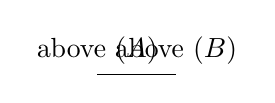
\begin{tikzpicture}
 \coordinate [label=above ($A$)] (A) at (0,0);
 \coordinate [label=above ($B$)] (B) at (1,0);
 
 \draw (A) -- (B);
 \end{tikzpicture}
 \item Uma superfície é aquela que só tem comprimento e largura.
 \item Os extremos de uma superfície são linhas.
 \item Superfície plana é aquela, sobre a qual assenta toda uma tinha reta entre dois pontos quaisquer, que estiverem na mesma superfície.
 \item Ângulo plano é a inclinação recíproca de duas linhas, qu se tocam em uma superfície plana, sem estarem em direitura uma com outra (sem estarem sobre uma mesma linha).
 \item Ângulo plano retilíneo é a inclinação recíproca de duas linhas retas, que se encontram, e não estão em direitura uma com outra.
 \item Um ângulo é a inclinação mutua de duas linhas que se encontram em um plano e não são colineares.
 \item Quando as línhas que compreendem o 

\end{enumerate}%Elementos de Euclides


%ENSINO SUPERIOR
%\chapter{Fundamentos da Matemática 1}

\section*{Recomendações Preliminares}
Algumas recomendações úteis:
\begin{itemize}
    \item Se inscreva no portal \url{https://pt.khanacademy.org/};
    \item Jogue jogos que envolvam raciocínio e tática como damas, xadrez, SUDOKU.
    \item Entre no portal \url{http://www.hypatiamat.com/} e jogue sempre que tiver tempo;
    \item Entre no portal \url{https://rachacuca.com.br/} para jogar jogos de raciocínio online;
    \item Baixe em seu computador o programa Geogebra.
    \begin{itemize}
        \item Navegue no portal \url{http://www.geogebra.im-uff.mat.br/index.html} e aprenda\linebreak como instalar o programa, ver como funciona através de vídeos tutoriais, além de acessar uma biblioteca com artigos sobre Geometria Dinâmica.
    \end{itemize}
    \item Se inscreva no portal \url{http://matematica.obmep.org.br/} e explore-o;
    \item Procure conhecer a coleção de Fundamentos da Matemática Elementar do Yezzi;
    \item Procure conhecer a coleção do Professor de Matemática da SBM;
\end{itemize}

\section{Revisão de Conjuntos}

\section*{Símbolos}

\begin{center}
\begin{tabular}{|c|c|}
\hline
$\in$ & pertence \\
\hline
$\not\in$ & não pertence\\
\hline
$\exists$ & existe \\
\hline
$\nexists$  & não existe \\
\hline
$\subset$  & está contido \\
\hline
$\not\subset$ & não está contido \\
\hline
$\forall$ & para todo \\
\hline
$\emptyset$  & conjunto vazio \\
\hline
$\supset$  & contém \\
\hline
$|$ & não está contido \\
\hline
$\longleftrightarrow $ & se e somente se \\
\hline
$\mathbb{N}$  & conjunto dos números naturais \\
\hline
$\mathbb{Z}$& conjunto dos números inteiros \\
\hline
$\mathbb{Q}$ & conjunto dos números racionais \\
\hline
$\mathbb{I}$ & conjunto dos números irracionais \\
\hline
$\mathbb{R}$ & conjunto dos números reais \\
\hline
\end{tabular}
\end{center}

\section{Relação de pertinência}

Cada aluno da classe tem uma mesma propriedade: estar na sala de aula. Assim, ao falarmos neste conjunto estabelecemos a possibilidade de averiguar se uma pessoa pertence ou não a ele. O conceito básico da teoria dos conjuntos é a relação de pertinência representada pelo símbolo $\in$. As letras minúsculas designam os elementos de um conjunto e as maiúsculas, os conjuntos. Assim, o conjunto das vogais $(V)$ é: $V = \{a, e, i, o, u\}$

\begin{itemize}
    \item A relação de pertinência é expressa por: $a \in V$, pois o elemento a pertence ao conjunto V.
    \item A relação de não-pertinência é expressa por: $b \not\in V$, pois o elemento b não pertence ao conjunto V.
\end{itemize}

\section{Formação de um conjunto}
Um conjunto pode ser definido de duas maneiras: enumerando seus elementos ou expressando uma ou mais propriedades que caracterízam todos os seus elementos.


\subsection{Enumerando elementos}
Aqui um conjunto seria expresso indicando cada um dos seus elementos. Por exemplo o conjunto $S$ a baixo.

 $S = \{1, 3, 5, 7, 9\}$
 
 Note que essa representação só é viável para o caso em que o conjunto é finito e, preferencialmente, com poucos elementos. Por exemplo temos os conjuntos que reunem soluções de equações. Uma equação de primeiro grau tem apenas uma solução. Uma equação quadrática tem até duas soluções.

\subsection{Expressando propriedades}

$S = \{\mbox{números ímpares de um algarismo}\}$ ou ainda
$S=\{x\in \mathbb{N};n=2x+1\mbox{ e } n\leq 9\}$

$B = \{x \in S / x \mbox{ tem a propriedade P}\}$; (lê-se: x pertence ao conjunto S tal que x possui a propriedade P).
O conjunto B é formado por todos os elementos de S que possuem a propriedade P.
Exemplo: $B = \{x \in \mathbb{N} / x < 8\} = \{0, 1, 2, 3, 4, 5, 6, 7\}$

Essa propriedade é conhecida no Raciocínio Lógico de Proposição Aberta. Uma proposição é uma afirmação a qual podemos sempre definir se seu valor lógico é Verdadeiro ou Falso. Para mais detalhes iremos dedicar uma seção no capítulo sobre Raciocínio Lógico com o tema Diagramas Lógicos.


\begin{defi}
Conjunto vazio: é um conjunto que não possui elementos. O conjunto vazio é representado por $\{ \ \}$ ou $\emptyset$.
\end{defi}

\begin{defi}
Subconjuntos: quando todos os elementos de um conjunto A qualquer pertencem a um outro conjunto B, diz-se, então, que A é um subconjunto de B, ou seja $$A\subset B$$.
\end{defi}

Observações:
\begin{itemize}
\item Todo o conjunto A é subconjunto dele próprio, ou seja $A\subset A$;
\item O conjunto vazio, por convenção, é subconjunto de qualquer conjunto, ou seja $\emptyset \in A$.
\item Se $A \subset B$ e $B\subset A$, então $A=B$.
\item Se $A \subset B$ e $B \subset C$, então $A\subset C$.
\end{itemize}

Logicamente podemos relacionar a inclusão de conjuntos com a implicação lógica. 

Seja a proposição $p(x):x$ é um número par e $q(x):x$ é um múltiplo de $4$. Temos duas proposições abertas. Serão verdadeiras ou falsas dependendo de quem dizemos ser $x$. Caso $x$ seja $6$, teremos que $p(6)$ será verdadeira enquanto $q(6)$ será falsa.

Perseba que todos os números multiplos de $4$ também são pares. Isso significa que $q\rightarrow p$ (lê-se ``$q$ implica $p$'').

Vamos colocar todos os números que tornam a proposição $q(x)$ verdadeira em um conjunto $Q$ e todos os que tornam a proposição $p(x)$ verdadeira em um conjunto $P$.

Teremos então:

$P=\{x\in \mathbb{N}; p(x)\}=\{0, 2, 4, 6, 8, \dots\}$

$Q=\{k\in \mathbb{N}; q(x)\}=\{0,4,8,12,16, \dots\}$

Teremos, $Q \subset P$, pois os multiplos de quatro é um subconjunto dos números pares.

Geralmente podemos aplicar conjuntos nas implicações lógicas e deduzir suas relações bem mais rápido que utilizando cálculo proposicional.

\section{Igualdade de conjuntos}

\subsection{Propriedades básicas}
Para todos os conjuntos $A$, $B$ e $C$, para todos os objetos $x\in U$, temos que:
\begin{enumerate}
    \item $A=A$;
    \item Se $A=B$, então $B=A$;
    \item Se $A=B$ e $B=C$, então $A=C$;
    \item Se $A=B$ e $x\in A$, então $x\in B$
    \item Se $A=B$ e $A\subset C$, então $B \subset C$.
\end{enumerate}

Dois conjuntos são igual se, e somente se, possuem exatamente os mesmos elementos não importando a ordem ou a repetição.

Dentro do raciocínio lógico teremos a dupla implicação. Ela é conhecida como ``se, e somente se...''. 

Seja p: x é um número multiplo de 2 e q: x é um número par.

Seja $P$ o conjunto dos números multiplos de 2 e $Q$ o conjunto dos números pares. 

Teremos que os conjuntos $P$ e $Q$ são iguais ($P=Q$), pois um número ser par implica que ele é multiplo de dois ($p \rightarrow q$) e um número ser multiplo de dois implica que ele é par ($q \rightarrow p$). Ou sejam um número é par se, e somente se, ele for multiplo de dois ($p\leftrightarrow q$).

\section{Conjunto complementar}

Complementar de $A$ com respeito a $R$ e é representada por $C^R_A = R - A$.

No caso dos alunos de uma classe, o conjunto complementar do conjunto dos alunos presentes à aula será formado pelos alunos ausentes à aula.


{\huge Observação}
\fbox{
\begin{minipage}{13cm}
Caso esteja claro em relação a quem é o complementar, então representamos o complementar de $A$ por $\bar{A}$
\end{minipage}
}

\section{Operações com conjuntos}

\begin{defi}   
União de Conjuntos: dados os conjuntos A e B, define-se como união dos conjuntos A e B ao conjunto representado por $A \cup B$, formado por todos os elementos pertencentes a A ou B, ou seja:
\end{defi}

\def\firstcircle{(0,0) circle (1.5cm)}
\def\secondcircle{(0:2cm) circle (1.5cm)}

\colorlet{circle edge}{blue!50}
\colorlet{circle area}{blue!20}

\tikzset{filled/.style={fill=circle area, draw=circle edge, thick},
    outline/.style={draw=circle edge, thick}}

\setlength{\parskip}{5mm}


\begin{figure}[h]

\centering
% Set A or B

\begin{tikzpicture}
    \draw[filled] \firstcircle node {$A$}
                  \secondcircle node {$B$};
    \node[anchor=south] at (current bounding box.north) {$A \cup B$};
\end{tikzpicture}

\caption{$A \cup B = \{x|x \in A\mbox{ ou }x\in B\}$}
\label{fig:uniao}
\end{figure}

%\def\firstcircle{(0,0) circle (0.5)}
%\def\secondcircle{(.7,0) circle (0.5)}

%\begin{tikzpicture}[xscale=2,yscale=2]

%\begin{scope}
%        \fill[blue] \firstcircle;
%        \fill[blue] \secondcircle;
        %\fill[blue] \thirdcircle;
%        \draw \firstcircle node[below] {$A$};
%        \draw \secondcircle node [above] {$B$};
        %\draw \thirdcircle node [below] {$C$};
%    \end{scope}


\begin{exe}
Ano: 2015 Banca: IBFC Órgão: MGS Prova: Nível Fundamental Incompleto

A união entre os conjuntos $A =\{ 0,1,2,3,4,5\}$ e $B = \{1,2,3,5,6,7,8\}$ é: 

\begin{multicols}{4}
\begin{enumerate}
    \item[a)] $\{0,1,2,3,5,6,7,8\} $
    \item[b)] $\{0,1,2,3,4,5,6,7,8\} $
    \item[c)] $\{1,2,3,4,5,6,7,8\} $
    \item[d)] $\{0,1,2,3,4,5,6,8\} $
\end{enumerate}
\end{multicols}
\end{exe}


\begin{defi}
Intersecção de Conjuntos: dados os conjuntos A e B, define-se como intersecção dos conjuntos A e B ao conjunto representado por $A\cap B$, formado por todos os elementos pertencentes a A e B, simultaneamente, ou seja:  

\end{defi}



\begin{figure}[h]
\centering

% Set A and B
\begin{tikzpicture}
    \begin{scope}
        \clip \firstcircle;
        \fill[filled] \secondcircle;
    \end{scope}
    \draw[outline] \firstcircle node {$A$};
    \draw[outline] \secondcircle node {$B$};
    \node[anchor=south] at (current bounding box.north) {$A \cap B$};
\end{tikzpicture}

\caption{$A\cap B=\{x|x\in A\mbox{ e }x\in B\}$}
\label{fig:my_label}
\end{figure}

\subsection{Número de Elementos da União}

$$n(A \cup B)=n(A)+n(B)-n(A\cap B)$$

\begin{defi}
Diferença de Conjuntos: dados os conjuntos A e B, define-se como diferença entre A e B (nesta ordem) ao conjunto representado por $A-B$, formado por todos os elementos pertencentes a A, mas que não pertencem a B, ou seja: 
\end{defi}

\begin{figure}[h]
\centering

%Set A or B but not (A and B) also known a A xor B
\begin{tikzpicture}
    \begin{scope}
        \clip \firstcircle;
        \draw[filled, even odd rule] \firstcircle node {$A$}
                                     \secondcircle;
    \end{scope}
    \draw[outline] \firstcircle
                   \secondcircle node {$B$};
    \node[anchor=south] at (current bounding box.north) {$A - B$};
\end{tikzpicture}

\caption{$A-B=\{x|x\in a\mbox{ e }x\not\in B\}$}
\label{fig:my_label}
\end{figure}

\begin{center}
 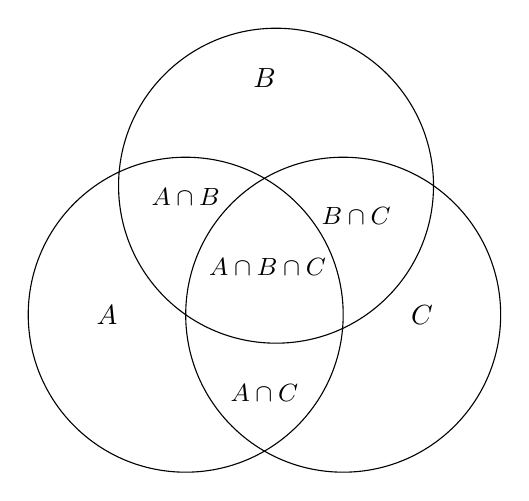
\begin{tikzpicture}

 \pagestyle{empty}

\def\firstcircle{(0,0) circle (2cm)}
\def\secondcircle{(55:2cm) circle (2cm)}
\def\thirdcircle{(0:2cm) circle (2cm)}

    \begin{scope}
      \clip \firstcircle;
      \clip \secondcircle;
      \fill[white] \thirdcircle;
    \end{scope}

    \draw \firstcircle;
    \node at (-1,0) {$A$};
    
    \draw \secondcircle;
    \node at (1,3) {$B$};
    
    \draw \thirdcircle;
    \node at (3,0) {$C$};
    
    \begin{scope}[font=\small]
     \draw(1,-1) node {$A\cap C$};
     \draw(90:1.5cm) node {$A\cap B$};
     \draw(30:2.5cm) node {$B\cap C$};
     \draw(30:1.2cm) node {$A\cap B\cap C$};
    \end{scope}
  \end{tikzpicture}
\end{center}


\begin{defi}
Produto Cartesiano: dados os conjuntos A e B, chama-se peoduto cartesiano A com B, ao conjunto $A\times B$, formado por todos os pares ordenados $(x,y)$, onde x é elemento de A e y é elemento de B, ou seja $$A\times B=\{(x,y)|x\in A\mbox{ e }y\in B\}$$ 
\end{defi}

%\subsection{Número de elementos - Probabilidade}
%\subsection{Número de elementos - Relacionado a porcentagem}

\subsection{Simplificação no cálculo proposicional}
A linguagem de conjuntos pode ser utilizado para simplificar e efetuar calculos lógicos. Como um conjunto pode ser definido como a coletividade de elementos de um certo universo predeterminado que satisfazem a uma proposição aberta bem definida. Por exemplo, no universo dos números naturais poderemos estabelecer o conjunto dos pares apenas tomando os elementos de $\mathbb{N}$ que tornam a proposição aberta ``\textit{P(x):x pode ser dividido por $2$}'' verdadeira.

Vejam que as operações entre conjuntos podem ser compreendidas como operações lógicas. Sendo assim uma equação proposicional pode ser modelada através de relações e operações entre conjuntos.



Agora vamos tomar um conjunto formado pelos números naturais menores ou iguais a um certo \textit{n}\footnote{$\{n,i\in \mathbb{N}; i\leq n\}$} e o representamos por $I_n=\{1,2, \dots, n\}$. Ou seja:

\begin{align*}
    I_1&=\{1\}\\
    I_2&=\{1,2\}\\
    I_3&=\{1,2,3\}\\
    \vdots &= \vdots \\
    I_n&=\{1,2,3, \dots , n\}
\end{align*}

\section*{Questões optativas}
\begin{enumerate}
\item Note que $I_1$ é subconjunto de $I_2$. E que $I_2$ é subconjunto de $I_3$. Logo temos que $I_1$ também é sunconjunto de $I_3$. Podemos generalizar e dizer que $I_n$ sempre será subconjunto de $I_m$ em que situração?

\item Note que a união de $I_1$ com $I_2$ é igual a $I_2$. E que a união de $I_2$ com $I_3$ é igual a $I_3$ (verifique). $I_1$ unido com $I_3$ será igual a quem? Quando eu posso dizer que a União de $I_n$ com $I_m$ é igual a $I_m$?

\item Quanto a intersecção de dois deles, relacione $I_1$ com $I_2$, depois $I_2$ com $I_3$ e depois $I_1$ com $I_3$. Quando que $I_n \cap I_m = I_m$?
\end{enumerate}

Note que o \textit{n} ao mesmo tempo que serve de indice para o conjunto \textit{I} ele diz quantos elementos tem em I (verifique).


Para o conjunto sem elementos temos temos que ele contem apenas um subconjunto, ele próprio. Para um sonjunto unitário ele possui dois sunconjuntos, um unitário e um vazio. Para um conjunto com dois elementos temos quatro subconjuntos: um vazio, dois unitário e um com dois elementos que é ele próprio. Seguindo essa orientação temos a seguinte tabela abaixo.\\

\begin{center}
  \begin{tabular}{|c|c|c|c|}
  \hline
       $A$  & $P(A)$ & Pascal &$|P(a)|$  \\
\hline
       $\{1\}$ & $\{ \emptyset , \{1\} \}$ & 1 \quad 1 & 2\\
\hline
$\{1,2\}$ & $\{ \emptyset , \{1\},\{2\}, \{1,2\} \}$ & 1 \quad 2 \quad 1 & 4\\
\hline
$\{1,2,3\}$& $\{ \emptyset , \{1\},\{2\},\{3\}, \{1,2\},\{1,3\},\{2,3\},\{1,2,3\} \}$ & 1 \quad 3 \quad 3 \quad 1  & 8\\
\hline

    \end{tabular}
\end{center}

A primeira coluna da matriz representa um conjunto $A$ qualquer com apenas um elemento na primeira linha, dois na segunda e assim por diante. Note que as regras para a quantidade de elementos e a forma de encontrar as partes desse conjunto não varia se forem mudados as espécies dos elementos de $A$, apenas se mudarem sua quantidade.

Na segunda coluna temos o conjunto das partes do conjunto $A$. Note que esse conjunto sempre contém o conjunto vazio e o próprio conjunto $A$. Sua composição será de todos os subconjuntos de $A$. Logo sua composição irá variar com subconjuntos vazio, com um elemento, dois elementos, etc até a quantidade total dos elementos de $A$ que é quando o próprio $A$ está contido nele. Mas a sua distribuição em relação a esses conjuntos é dada pela terceira coluna.

A terceira coluna que chamei de "Pascal" enumera em seu primeiro termo a quantidade de conjuntos vazios (sempre 1), en seu segund termo a quantidade de conjuntos unitários (1 na primeira linha, 2 na segunda, etc), no terceiro termo temos a quantidade de conjuntos com dois elementos. Ou seja, para o n-ésimo termo (quando o tiver) ele indicará a quantidade de subconjuntos de $A$ com $n-1$ elementos.

A quarta coluna indica a quantidade total dos elementos das partes do conjunto $A$. Note que há um padrão nessa numeração. Qual padrão é esse?



\begin{defi}
Número de subconjuntos de um conjunto: se um conjunto A possuir n elementos, então existirão $2^n$ subconjuntos de A.
 \end{defi}
 

 \begin{center}
$\begin{matrix} 1 \\ 1 \quad 1 \\ 1 \quad 2 \quad 1 \\ 1 \quad 3 \quad 3 \quad 1 \\ 1 \quad 4 \quad 6 \quad 4 \quad 1 \\ 1 \quad 5 \quad 10 \quad 10 \quad 5 \quad 1 \\ 1 \quad 6 \quad 15 \quad 20 \quad 15 \quad 6 \quad 1 \\ 1 \quad 7 \quad 21 \quad 35 \quad 35 \quad 21 \quad 7 \quad 1 \\ 1 \quad 8 \quad 28 \quad 56 \quad 70 \quad 56 \quad 28 \quad 8 \quad 1 \\ 1 \quad 9 \quad 36 \quad 84 \quad 126 \quad 126 \quad 84 \quad 36 \quad 9 \quad 1 \\ 1 \quad 10 \quad 45 \quad 120 \quad 210 \quad 252 \quad 210 \quad 120 \quad 45 \quad 10 \quad 1 \\ 1 \quad 11 \quad 55 \quad 165 \quad 330 \quad 462 \quad 462 \quad 330 \quad 165 \quad 55 \quad 11 \quad 1 \\ 1 \quad 12 \quad 66 \quad 220 \quad 495 \quad 792 \quad 924 \quad 792 \quad 495 \quad 220 \quad 66 \quad 12 \quad 1 \end{matrix}$
\end{center}

\section{Revisão de Equações}
O objetivo é revisar equações com uma introdução as funções. 

Lembre-se que uma expressão aritmética pode ser tanto uma função como uma equação. Note ainda que a equação nada mais é que um caso espefícifo da função. Quando temos uma expressão igualada a zero temos o ponto em que a função toca o eixo $x$.

\subsection{Equação do Primeiro Grau}
Faça diversas equações para valores consecutivos para, assim, introduzir a função pela \linebreak Progressão Aritmética. Contextualize com a função horária das posições para o movimento retilíneo uniforme e uniformemente variado para mostrar que a posição inicial seria o primeiro termo, a razão seria a velocidade e a posição final seria o termo geral.

\subsection{Equação do Seundo Grau}

Uma equação é toda igualdade em que de um lado temos uma expressão algébrica e do outro um resultado. No caso das equações quadráticas (outro nome dado para as equações do $2^o$ grau), teremos de uma expressão polinomial de grau dois igualado a zero.

\begin{equation}\label{1.1}
    ax^2+bx+c=0
\end{equation}

Para a resolução de equações desse gênero é conhecida fórmula de báscara que visa obter o valor das raízes em função dos coeficientes $a$, $b$ e $c$. A fórmula em questão é a de Bhaskara\footnote{Matemático Indiano do Século XII} e é expressa por

\begin{equation}\label{1.2}
    x=\dfrac{-b \pm \sqrt{\Delta}}{2a}
\end{equation}

em que $\Delta$ é o discriminante, e vale
\begin{equation}\label{1.3}
    \Delta=b^2-4ac.
\end{equation}

A fórmula acima pode ser deduzida a partir do processo de completar quadrado sobre a equação \eqref{1.1}.

\begin{exe}
Encontre o resultado da equação quadrática $2x^2-3x-1=0$
\end{exe}
O primeiro passo é identificar os coeficientes. 
\begin{align*}
    a&=2\\
    b&=-3\\
    c&=1
\end{align*}

Assim que identificamos os coeficientes passamos para encontrar o valor do discriminante.

\begin{align*}
    \Delta&=(-3)^2-4\cdot 2 \cdot 1\\
    &=9-8=1
\end{align*}

Basta agora substituir os valores do discriminante e dos outros termos em \eqref{1.2}.

\begin{align*}
    x&=\dfrac{-(-3)\pm \sqrt{1}}{2\cdot 2}\\
    &=\dfrac{2\pm 1}{4}
\end{align*}    
 
 Como o valor do discriminante é maior que zero teremos duas soluções diferentes.
 \begin{align*}
    \begin{cases}
    x'=\frac{3}{4}\\
    x''=\frac{2}{4}=\frac{1}{2}
    \end{cases}
 \end{align*}
 
 Para os casos em que o discriminante é zero, então teremos uma única solução. Quando o discriminante é negativo nós não teremos soluções reais.
 
 Apesar de podermos utilizar esse método para resolver quaisquer equações quadráticas, podemos economisar tempo em casos especiais.
 
 \subsection{Caso em que $b=0$}
 Nesse tipo de caso a equação \label{1.1} torna-se
 
 \begin{equation}\label{1.4}
     ax^2+c=0.
 \end{equation}
 Para esse tipo de situação basta isolar o termo quadrático e, por fim, retirar a raiz quadrada.
 
 \begin{align*}
     ax^2&=-c\\
     x^2&=-\dfrac{c}{a}\\
     x&=\pm \sqrt{-\dfrac{c}{a}}
 \end{align*}
 
 Geometricamente podemos representar esse caso com a figura abaixo
 
 FIGURA REPRESENTATIVA DE DIFERENÇA DE QUADRADOS
 
 
 \subsection{Caso e que $c=0$}
 Nesse caso a equação \label{1.1} torna-se
 
 \begin{equation}\label{1.5}
     ax^2+bx=0.
 \end{equation}
 
 Aqui podemos isolar o valor de $x$. Ficamos com 
 
 \begin{align*}
     x(ax+b)=0     
 \end{align*}
 
 que tem como solução apenas $x=0$ e $x=\frac{-b}{a}$.

REPRESENTAÇÃO GEOMÉTRICA
Função horária das posições para o movimento uniformemente variádo.

Progressão aritmética de segunda ordem. Problemas com sequências numéricas.

\section{Introdução as Funções}%Fundamentos 1
%%%%%%%%%%%%%%%%%%%%%%%%%%%%%%%%%%%%%%%%%%%%%%%%%%%%
\chapter{Geometria Analítica}

\begin{defi}
Círculo $C$ de centro $A\in \pi$ e raio $r>0$ é o conjunto de pontos do plano $\pi$ situados à distância $r$ do ponto $A$, ou seja $$C=\{P\in \pi ;d(P,A)=r \}$$
\end{defi}

\begin{center}
\begin{tikzpicture}[scale=1]
\coordinate [label={below right:$A$}] (A) at (2,2);
\coordinate [label={below right:$P$}] (P) at (2,3);

\draw[->] (0,-.5)--(0,4);
\draw[->] (-.5,0)--(4,0);

\draw (A) circle (1cm);
\draw[fill=black] (A) circle (0.4mm);
\draw[fill=black] (P) circle (0.4mm);
\end{tikzpicture}
\end{center}

MEDIATRIS DO SEGMENTO AB%Geometria Analítica
%%%%%%%%%%%%%%%%%%%%%%%%%%%%%%%%%%%%%%%%%%%%%%%%%%%
\chapter{Introdução a Lógica}



Algumas recomendações:
\begin{itemize}
    \item Acesse o portal \textit{Racha Cuca}\footnote{https://goo.gl/U9V8jH} e joge diversos jogos, especialmente:
    \begin{multicols}{2}
        \begin{itemize}
        \item Quase Nada;
        \item Cubo vermelho;
        \item Pinguins Numa Fria;
        \item Missionários e Canibais;
        \item Problemas de Lógica;
        \item Jógos de Lógica;
        \item Sudoku;
    \end{itemize}
    \end{multicols}
    \item Acesse o portal \textit{Geniol}\footnote{https://www.geniol.com.br/logica/} e jogue:
    \begin{multicols}{2}
    \begin{itemize}
        \item Sudoku;
        \item Desafios de Lógica;
        \item Tangran;
        \item Encaixe Perfeito;
    \end{itemize}
    \end{multicols}
    \item Acesse o portal \textit{Questões de Concursos}\footnote{www.qconcursos.com}. Clique na aba \textit{Questões} e depois aplique Raciocínio Lógico na Disciplina e responda questões ou filtre por algum assunto de preferência primeiro.
    \item Acesse o portal \textit{Passei Direto}\footnote{www.passeidireto.com} e procure alguns materiais como:
    \begin{itemize}
        \item Raciocínio Lógico Simplificado de Sérgio Carvalho Vl 1 e Vl 2;
        \item Notas de Aulas de Lógica do professor Joselias;
    \end{itemize}
\end{itemize}

\section{Fundamentos de Lógica}

Segundo Irving Copi lógica é: ``uma ciência do raciocínio'' pois a sua ideia está ligada ao processo de raciocínio correto e incorreto que depende da estrutura dos argumentos envolvidos nele. Assim concluimos que a lógica estuda as formas ou estruturas do pensamento, isto é, seu propósito é estudar e estabelecer propriedades das relações formais entre as proposições.

\subsection{Proposições Simples e Compostas e Operadores Lógicos}

Chama-se frase a todo conjunto de palavras ou símbolos que expressam um pensamento ou uma ideia de sentido completo. 

Para as frases que transmitem afirmação de fatos ou exprimem juízos que formamos a respeito de determinados conceitos ou entes denominamos \textbf{proposição}. Esses fatos ou juízos afirmados pela proposição em questão deverão sempre ter um valor verdadeiro (V) ou um valor falto (F), senão  a frase em si não contituirá uma proposição lógica, e sim apenas uma frase.

\begin{exe}
O Profssor Antônio é bonito.
\end{exe}




\subsection{Tabelas verdade, tautologia, contadição e Contingência}

\section{Equivalência lógica e Negação de Proposições}

\subsection{Negação-Leis de Morgan (Negativa de uma proposição Composta)}
\subsection{Equivalência - Proposições Logicamente Equivalentes}

\section{Lógica de Argumentação - Diagramas e Operadores Lógicos}

\section{Implicação Lógica}

\section{Verdades e Mentiras}

\section{Diagramas de Venn (Conjuntos)}

\section{Quantificadores}

\section{Análise Combinatória}

\section{Problemas Lógicos com Dados, Figuras e Palitos}

\section{Sequências Lógicas de Números, Letras, Palávras e Figuras}

\section{Problemas Lógicos}

\section{Raciocínio Matemático}%Introdução a Lógica
%\chapter{Fundamentos da Matemática 2}

\section{Trigonometria}

\begin{equation}\label{4.1}
   f(x)=a\sin(bx) 
\end{equation}


O valor de $a$ indica a amplitude e $b$ indica a frequência. O inverso da frequência é o período.

\section{Funções Periódicas}

\begin{defi}
Uma função $f$ é dita periódica se existe um número real positivo $P$ chamado período de $f$, tal que

\begin{equation}\label{4.2}
f(x)=f(x+P)
\end{equation}
\end{defi}

INCLUIR FIGURA 1: UMA FUNÇÃO PERIÓDICA

Observações:

\begin{itemize}
    \item O período $P$ é o comprimento do intervalo em $x$ necessário para a imagem da função se repetir.
    \item Segue da \eqref{4.2} que se $f$ é periódica de período $P$, então para qualquer $n$ inteiro positivo temos
    
\begin{equation}\label{4.3}
    f(x)=f(x+nP)
\end{equation}

ou seja, qualquer múltiplo inteiro positivo $nP$ DE $P$ é um período de $f$. O menor valor de $P$ que satisfaz a equação \eqref{4.2} é chamado \textit{Período Fundamental} de $f$ e será denotado por $T$. Qualquer outro período de $f$ será um múltiplo inteiro do período fundamental.

\item A frequência $F$ de uma função periódica é definida como o inverso de seu período

CONTINUA: MATERIAL SOBRE INTRODUÇÃO AS SÉRIES DE FOURIER

\end{itemize} 

\section{Números Complexos}
O que é um número complexo? O adjetivo complexo é infeliz, herdado de épocas nas quais a abstração envolvida na compreensão desses números era considerada elevada. Atualmente sabemos que o conceito de número real exige núvel de abstração equivalente e, para exemplificar isso, começamos trabalhando a mais básica ilustração que se pode dar sobre números completos: a ssolução da equação

$$X^2+1=0 \mbox{ ou, o que dá no mesmo, } X^2=-1$$

Sabemos que sobre $\mathbb{R}$ não há solução e somos forçados a definir um ``número'' $i$, satisfazendo $i^2=-1$, que resolve a equação. Agora, ou postulamos a existência desse ``número'' ou invocamos a Álgebra Linear elementar e saimos em busca de um entre de natureza geométrica que seja a solução procurada. Se assim fizermos e olharmos para essa equação sob a forma

$$X \cdot X = -I$$

onde $X$ é uma matriz $2 \times 2$ com coeficientes reais, $I=$

CONTINUAR CAPÍTULO 1 DO LIVRO DE CÁLCULO EM UMA VARIÁVEL COMPLEXA


Você compreende a expressão $e^{i\pi}=-1$\footnote{\url{https://goo.gl/MXgoNy}}?

Na expressão em questão temos a participação de quatro elementos, a base do logaritmo natural, o valor de pi e a constante imaginátia dos números complexos.

Quando derivamos uma função exponencial $a^x$ obtemos como resultado um múltiplo dela. Logo para que a derivada de uma função exponencial seja igual a ela própria basta que o valor pelo qual multiplico a minha funçã após a derivada seja $1$. Esse valor em questão é uma expressão que envolve o limite no infinito. Deduza a expressão $e=\lim_{n \to \infty} \left( 1+\dfrac{1}{n} \right)^n$ a partir da derivada da função exponencial pela definição de derivada.

Verifique que $e^x=\lim_{n \to \infty} \left( 1+\dfrac{x}{n} \right)^n$.

Note que agora substituindo o valor de $\pi$ no lugar do $x$ encontraremos algo que se aproxima muito da expressão.

$e^{\pi}=\lim_{n \to \infty} \left( 1+\dfrac{\pi}{n} \right)^n$

Agora estamos a um passo de obter o que queremos.

$e^{i\pi}=\lim_{n \to \infty} \left( 1+i\dfrac{\pi}{n} \right)^n$

Basta verificar o valor do limite acima e obter o resultado $-1$.

%Fundamentos 2
%\chapter{Cálculo 1}
\section{Limites}

%http://www.sistemaaguia.com.br/downloads/24-aplim.pdf
%http://www.dm.ufscar.br/profs/sampaio/calculo1_aula04.pdf
%http://www.dm.ufscar.br/profs/sampaio/calculo1_aula05.pdf
%http://sinop.unemat.br/site_antigo/prof/foto_p_downloads/fot_7567aula_1_-_limites_-_1_slide_pob_folha_pdf.pdf
%http://www.im.ufrj.br/~puignau/Calculo1/exos/2011-2/capitulo4.pdf

\section{Derivadas}

\subsection{Velocidade}
A velocidade é a razão entre a distância percorrida entre dois pontos e o tempo gasto. Quando dirigimos dificilmente mantemos a mesma velocidade, logo temos apenas a velocidade média.

GRÁFICO DA FUNÇÃO HORÁRIA DAS POSIÇÕES.

A VELOCIDADE É O COEFICIENTE DA INCLINAÇÃO DA RETA TANGENTE



A derivada pode ser compreendida como a inclinação da reta tangente de um ponto.


Equação da reta: $y-y_0=m(x-x_0)$

Inclinação da reta: $m=\dfrac{y-y_0}{x-x_0}$

Inclinação entre dois pontos de uma curva: $m_{AB}=\dfrac{f(x)-f(x_0)}{x-x_0}$

Inclinação da reta no ponto tangente: $m=\lim_{x\rightarrow x_0} =\dfrac{f(x)-f(x_0)}{x-x_0}$

Seja $h=x-x_0$, temos:
\begin{equation}\label{5.1}
    f'(x)=\lim_{h \rightarrow 0}\dfrac{f(x+h)-f(x)}{h}
\end{equation}

\subsection{Primeiras consequências}

DERIVADA DE CONSTANTE É ZERO

DERIVADA DE UMA FUNÇÃO VEZES UMA CONSTANTE É A CONSTANTE VEZES A DERIVADA DA FUNÇÃO

A DERIVDA DA SOMA(OU DIFERENÇA) ENTRE DUAS FUNÇÕES É A SOMA (OU DIFERENÇA) ENTRE SUAS DERIVADAS

\begin{table}[h]
    \centering
    \begin{tabular}{|c|c|}
    \hline
    Função & Derivada \\
    \hline
    $x^n$  & $nx^{n-1}$ \\
    \hline
    $\sin x $ & $\cos x$\\
    \hline
    $\cos x$ & $-\sin x$\\
    \hline
    $a^x$ & $a^x \ln a$\\
    \hline
    $\ln x$ & $1/x$ \\
        \hline
    \end{tabular}
    \caption{Tabela de derivadas}
    \label{tab:my_label}
\end{table}

\section{Derivada de função exponencial}

Seja $f(x)=x^n$ temos.

Substituindo nossa função na equação $\eqref{5.1}$, teremos

\begin{equation}\label{5.2}
    \lim_{h \to 0} \dfrac{(x+h)^n-x^n}{h}
\end{equation}

\section{Derivada de função exponencial}

Seja $f(x)=a^x$ com $a>0$ e $a\not= 1$, vamos encontrar a sua derivada.

\begin{equation}\label{5.3}
\begin{split}
f'(x)&=\lim_{h \to 0}\dfrac{f(x+h)-f(x)}{h}\\
&=\lim_{h \to 0}\dfrac{a^{x+h}-a^h}{h}\\
&=\lim_{h \to 0}\dfrac{a^x\cdot a^h-a^x}{h}\\
&=\lim_{h \to 0}\dfrac{a^x(a^h-1)}{h}\\
&=\lim_{h \to 0}\dfrac{a^x(a^h-1)}{h}\\
&=a^x\cdot \lim_{h \to 0}\dfrac{a^h-1}{h}
\end{split}
\end{equation}

Nota-se que a derivada de uma função exponencial é um múltiplo da própria função. Será que existe uma função exponencial cuja derivada seja ela própria? Para que isso ocorra basta que o limite em questão seja $1$.

\begin{equation}\label{5.4}
\begin{split}
\lim_{h \to 0}\dfrac{a^h-1}{h}&=1\\
\lim_{h \to 0}a^h-1&=h\\
\lim_{h \to 0}a^h&=h+1\\
a&=\lim_{h \to 0}(h+1)^{\frac{1}{h}}
\end{split}
\end{equation}

Fazendo $\dfrac{1}{h}=n$ teremos

\begin{align}\label{5.5}
a&=\lim_{n\to\infty}\left(1+\dfrac{1}{n}\right)^n
\end{align}

Esse limite converge para um número irracional que será conhecido como número de Euler e será representado por $e$.

Observe que a derivada genéria de uma função exponencial é $(a^x)'=a^x \ln (a)$ e que np caso específico de $a=e$ teremos $(e^x)'=e^x\ln(e)$. Mas como $\ln(e)=1$ voltamos para $(e^x)'=e^x$.

Outra coisa a considerar é que o limite que aparece em (5.6) identifica o $\ln(a)$. Ou seja

$$ln(a)=\lim_{h \to 0}\dfrac{a^h-1}{h}$$

\section{Técnicas de Derivação}

\subsection{Regra do produto}
$$(ab)'=a'b + b'a$$


\begin{align}\label{5.6}
    \lim_{h \rightarrow 0} \dfrac{d (f(x)g(x))}{dx}&=\lim_{h\rightarrow 0} \dfrac{f(x+h)g(x+h)-f(x)g(x)}{h}
\end{align}

Tomando $f(x+h)=f(x)+\delta f$ e $g(x+h)=g(x)+\delta g$, temos

\begin{equation}\label{5.7}
\begin{split}
&=\lim_{x\rightarrow 0} \dfrac{(f(x)+\delta f)(g(x)+\delta g)-f(x)g(x)}{h}\\
&=\lim_{x\rightarrow 0} \dfrac{f(x)\delta g +g(x)\delta f + \delta f \delta g}{h}
\end{split}
\end{equation}

Como as variações $\delta f$ e $\delta g$ são muito pequenas podemos ignorá-las. Dessa forma basta devolver a anotação que utiliza o delta para a anterior e verificar a afirmação dada inicialmente.

\subsection{Regra da Cadeia}


\begin{equation}\label{5.8}
f(g(x))'=f'(g(x))g'(x)
\end{equation}



\subsection{Regra do Quociente}

\begin{equation}\label{5.9}
\left( \dfrac{a}{b} \right)'=\dfrac{b'a-a'b}{b^2}
\end{equation}


Utilizando:

\begin{itemize}
\item $\frac{f(x)}{g(x)}=f(x)g(x)^{-1}$
\item $\frac{d(f(x))}{dx}=f'(x)$
\item $(u^{-1})'=-u^{-2}$
\end{itemize}

\begin{align*}
    \dfrac{d(f(x)[g(x)]^{-1})}{dx}&=\dfrac{d(f(x))}{dx}[g(x)]^{-1}+\dfrac{d([g(x)]^{-1})}{d(x)}f(x)
\end{align*}

Ou ainda

\begin{align*}
    &=f'(x)g(x)^{-1}+(g(x)^{-1})'f(x)\\
    &=f'(x)g(x)^{-1}-g(x)^{-2}g'(x)f(x)\\
    &=\dfrac{f'(x)}{g(x)}-\dfrac{g'(x)f(x)}{g(x)^2}
\end{align*}

Multiplicando a primeira fração por $g(x)$ e subtraindo a segunda obtemos o que estavamos procurando.

%Cálculo 1
%\chapter{Algebra Linear}

\section{Operações Vetoriais}
ADIÇÃO DE DOIS VETORES

PRODUTO POR UM ESCALAR

\subsection{Produto Escalar de dois vetores}

\begin{equation}\label{6.1}
    \textbf{A} \cdot \textbf{B} = AB \cos \theta
\end{equation}

COMUTATIVA

DISTRIBUTIVA
\begin{equation}\label{6.2}
    \textbf{A} \cdot (\textbf{B}+\textbf{C})=\textbf{A} \cdot \textbf{B}+\textbf{A} \cdot \textbf{C}
\end{equation}

PRODUTO VETORIAL DE DOIS VETORES

\section{Vetor na forma de componentes retângulares}

PRODUTO TRIPLO

\section{Giro dos Eixos Coordenados}\nocite{weber2003essential}

\begin{equation}\label{6.3}
\begin{split}
    (x,y)&=x(1,0)+y(0,1)\\
    &=x(\cos \phi , \sin \phi)+y(-\sin \phi , \cos \phi)\\
    &=(x\cos \phi - y\sin \phi, x \sin \phi +  \cos \phi )
    \end{split}
\end{equation}

As coordenadas do ponto $P(x,y)$ após girar $\phi$ graus envolta da origem terá (em relação ao plano). Ou seja, temos após o giro:
\begin{center}
 $P'= \begin{cases}
x'=x\cos \phi - y\sin \phi \\ 
y'= x \sin \phi +  y\cos \phi
\end{cases}$
\end{center}
Ou ainda

$$\left( \begin{matrix} x' \\ y' \end{matrix} \right)=\begin{bmatrix} \cos \phi & \sin \phi \\ -\sin \phi  & \cos \phi \end{bmatrix}\left( \begin{matrix} x \\ y \end{matrix} \right) $$

Quanto é o plano e não o ponto que gira entorno da origem então é como se o ponto girasse no sentido oposto do ponto de vista do plano. Ou seja, se o plano gira $\phi$ graus e o ponto \textit{P} permanece parado então é como se o plano tivesse se mantido parado e o ponto tivesse girado $-\phi$ graus, ou girado $\phi$ no sentido oposto. Logo teremos

\begin{equation}\label{6.4}
\begin{split}
    (x',y')&=x(\cos (-\phi) , \sin (-\phi))+y(-\sin (-\phi) , \cos (-\phi))\\
    &=x(\cos \phi , -\sin \phi)+y(\sin \phi , \cos \phi)\\
    &=(x\cos \phi + y\sin \phi,- x \sin \phi + y \cos \phi )
    \end{split}
\end{equation}

Ou seja:

\begin{center}
$ P'= \begin{cases}
x'=x\cos \phi + y\sin \phi \\ 
y'=- x \sin \phi + y \cos \phi
\end{cases}$
\end{center}

Podemos deduzir essa mesma fórmula apartir da imagem abaixo. Note que temos dois triângulos retângulos em que as hipotenusas são a coordenada e a abscissa.  Note ainda que o ângulo mais agudo de ambos corresponde a $\phi$. 

\begin{figure}[h]
    \centering
    \includegraphics[scale=.5]{./imagens/09.png}
    \caption{Coordenadas de um ponto em um plano rotacionado}
    \label{fig:my_label}
\end{figure}


%Álgebra Linear
%%%%%%%%%%%%%%%%%%%%%%%%%%%%%%%%%%%%%%%%%%%%%%%%%%%
\chapter{Fatoração}

\section{Por em Evidência}

\begin{align}
    a+ab&=a(1+b)\\
    a^2b+ab^2&=ab(a+b)
\end{align}

\section{Agrupar}

\begin{align}
    ac+ad+bc+bd&=a(c+d)+b(c+d)\\
    &=(a+b)(c+d)\\
    2ac-2bc+4ad-bc&=2a(c+2d)-3bc
\end{align}

%\end{figure}%Geometria Euclidiana 1
%%%%%%%%%%%%%%%%%%%%%%%%%%%%%%%%%%%%%%%%%%%%%%%%%%%%%%%%
\chapter{Cálculo 2}

A integral é uma soma de Himam infinitesimal.

\begin{equation}\label{8.1}
    \int_a^b f(x) dx = \lim_{n \to \infty} \sum_{  i=1}^{n  }{ f(x_i) \Delta x } 
\end{equation}

em que $x_i=a+i\Delta x$ e $\Delta x=\dfrac{b-a}{n}$

\section{Técnicas de Integração}



%Cálculo 2
%%%%%%%%%%%%%%%%%%%%%%%%%%%%%%%%%%%%%%%%%%%%%%
\chapter{Geometria Euclidiana 2}


%Geometria Eucl. 2
%%%%%%%%%%%%%%%%%%%%%%%%%%%%%%%%%%%%%%%%%%%%%%
\chapter{Introdução a Teoria dos Números}
%http://www.mat.unb.br/~maierr/tnotas.pdf
%http://wwwp.fc.unesp.br/~mauri/TN/SistNum.pdf O SISTEMA TERNÁRIO É O SISTEMA DE MAIOR CAPACIDADE
\section{Resultados Preliminares}
\subsection{O princípio da indução}
\subsection{O teorema binomial}
\subsection{Os números triangulares}
\section{Teoria de divisibilidade nos inteiros}
\section{Números primos e sua distribuição}
\section{Triplos PITAGORICOS e a conjctura de FERMAT}
\section{Números deficientes-abundantes-perfeitos e de MERSENNE}

Os números primos de Mersenne são casos particulares do mito da origem do xadrez.

%https://pt.wikipedia.org/wiki/Primo_de_Mersenne

\section{A teoria das congruências}
Escolha dois competidores. Um deles escolherá dentre duas opções -- ``1'' ou ``2''-- e acrescentará uma ou duas unidades mentalmente vocalizando apenas o resultado. Ganha o primeiro que que chegar ao número ``20''.

Existe alguma forma de vencer sempre?


\subsection{Teorema Chinês do Resto}
O Teorema Chinês do Resto é a evolução do que conhecemos como Menor múltiplo comum. Ambos se equivalem se estivermos trabalhando com restos iguais a zero no Teorema Chinês do Resto.

\section{Os Teoremas de FERMAT e WILSON}




%Introd. Teoria dos Núm.
%\chapter{Introdução a Computação}



%https://pt.wikiversity.org/wiki/Introdu%C3%A7%C3%A3o_%C3%A0_Ci%C3%AAncia_da_Computa%C3%A7%C3%A3o

%http://www.w3schools.com/html/default.asp

%http://www.ferrari.pro.br/home/documents/FFerrari-CCechinel-Introducao-a-algoritmos.pdf

%https://python.ime.usp.br/panda/default/index

%http://www.ime.usp.br/~hitoshi/introducao/

%http://www.ime.usp.br/~pf/algoritmos-livro/

%http://ccsl.ime.usp.br/files/books/intro-java-cc.pdf

%https://panda.ime.usp.br/pensepy/static/pensepy/index.html

%https://panda.ime.usp.br/aulasPython/static/aulasPython/index.html

%http://interactivepython.org/runestone/static/pythonds/index.html

%https://panda.ime.usp.br/algoritmos/static/algoritmos/index.html

\section{Notação Polonesa Reversa}

\section{Pyton}

%Introd. Computação
%%%%%%%%%%%%%%%%%%%%%%%%%%%%%%%%%%%%%%%%%
\chapter{Cálculo 3}
\section{Curvas Parametrizadas}
\subsection{Comprimento de Arco e Curvatura}

\begin{equation}\label{12.1}
    L=\int_a^b \sqrt{1+\left(\frac{df}{dx}\right)^2} dx
\end{equation}
\section{Funções de Várias Variáveis}

\section{Derivação de funções de várias variáveis}

\subsection{Derivadas Parciais}
\subsection{Diferenciais}
\subsection{Derivada Direcional}
\subsection{Gradiente}

\section{Máximos e Mínimos}


%Cálculo 3

%%%%%%%%%%%%%%%%%%%%%%%%%%%%%%%%%%%%%%%%%
\chapter{Álgebra Abstrata}

\section{Relações Aplicações e Operações}

\subsection{Relações Binárias}

\begin{defi}
Dados dois conjuntos $E$ e $F$, não vazios, chama-se produto cartesiano de $E$ por $F$ o conjunto pormado por todos os ``pares ordenados'' $(x,y)$ com $x$ em $E$ e $y$ em $F$, Costuma-se indicar o produto cartesiano de $E$ por $F$ com a notação $E\times F$ (lê-se:``$E$ cartesiano $F$''). Assim, temos:

\begin{equation*}
    E\times F=\{(x,y); x\in E \mbox{ e }y \in F\}
\end{equation*}
\end{defi}

\begin{defi}
Chama-se relação binária de $E$ em $F$ todo subconjunto $R$ de $E \times F$.
\end{defi}

\subsection{Relações de Equivalência}

\subsection{Relaçoes de Ordem}

\section{Grupos}
\paragraph{Teorema de Noethe} Para cada simetria da natureza corresponde uma lei de conservação (e vice-versa).

Transformações simétricas em relação a translação espacial implica na conservação do momentum. As do tempo na conservação de Energia. As de rotações nas de momento angular.

Outro tipo são as transformações de Gauge no Eletromagnetismo que implicam na conservação de carga.

O conjunto de operações de simetria formam um grupo e tem as seguinte propriedades:


\section{Anéis e Corpos}

\section{Anéis de Polinômios}

\subsection{Sequências}
\begin{defi}
Sequência é toda função definida no conjunto $\mathbb{N}^*$
\end{defi}

\paragraph{Igualdade:}

\paragraph{Adição:}

\paragraph{Multiplicação:}

\subsection{Sequências quase-nulas ou polinômios}

\begin{defi}
Dado um anel $A$, uma sequência $()$ sobre $A$ recebe o nome de \textit{polinômio sobre $A$} se existe um índice $r\in \mathbb{N}$ tal que $a_m=0$ para todo $m> r$.
\end{defi}

\paragraph{Proposição 1:}

\paragraph{Proposição 2:}

\subsection{Grau de um polinômio}

\begin{defi}
Seja $f=(a_i)$ um polinômio ...
\end{defi}



\subsection{Imersão de A em A[X]}



\subsection{Divisão em A[X]}



\subsection{Raízes de Polinômios}



\subsection{Polinômios sobre Corpos}

POLINÔMIOS IRREDUTÍVEIS

\begin{defi}
Seja $K$ um corpo. Dizemos que um polinômio $p\in K[X]$ é irredutível em $K[X]$ ou irredutível sobre $K$ se

\begin{enumerate}
    \item[(i)]  $p\in K$ (ou seja, $p$ não é um polinômio constante);
    \item[(ii)] Dado $f \in K[X]$, se $f|p$, então ou $f \in K^*$ ou existe $c \in K^*$ tal que $f=cp$.
\end{enumerate}
\end{defi}

Um polinômio $g \in K[K]$, não constante e não irredutível, chamase \textit{redutível} ou \textit{composto}.%Álgebra Abstrata
%%%%%%%%%%%%%%%%%%%%%%%%%%%%%%%%%%%%%%%%%%
\chapter{Física 1}
%http://sites.ifi.unicamp.br/f128/aulas/
%http://sites.ifi.unicamp.br/f128/ementa/
\section{Fórmulas Matemáticas}

\subsection{Movimento Retilíneo}

\begin{equation}\label{14.1}
    s=s_0+vt
\end{equation}

\subsection{Vetores}

O que é uma grandeza escalar?

Uma grandeza escalar é somente magniture; ela é apenas o número, positivo ou negativo.

O que é uma grandeza vetorial?

Uma grandeza vetorial é a junção de magniture com direção. Por exemplo, um cor se move para a direção sul a 40 km/h tem uma velocidade vetorial de 40km/h apontando para o sul.

SOMA VETORIAL

DESCRIÇÃO DE FUNÇÕES TRIGONOMÉTRICAS NO TRIÂGULO RETÂNGULO

COMPONENTES RETANGULARES DE UM VETOR.

ADIÇÃO DE VETORES POR SUAS COMPONENTES RETANGULARES.

PRODUTO DE VETOR POR ESCALAR

VETORES EM TRÊS DIMENSÕES: PRODUTO ESCALAR E VETORIAL

\subsection{Equilíbio de Forças Concorrentes}

CORDAS, NÓS E POLIAS SEM FRICÇÃO

FRICÇÃO E PLANOS INCLINADOS

\subsection{Cinemática Unidimencinal}

PROBLEMAS DE ACELERAÇÃO CONSTANTE

\begin{exe}
Um corpo com velocidae inicial de 8m/s se move em linha reta com aceleração constante e percorre 640 metros em 40 segundos. Para o intervalo de 40 segundos, encontre \textbf{a)} a velocidade média, \textbf{b)} a velocidade final, e \textbf{c)} a aceleração.
\end{exe}

A velocidade varia linearmente em função do tempo.
\begin{equation}\label{14.2}
v=v_0+at    
\end{equation}

Integrando em função do tempo, teremos a função posição para o movimento uniformemente variado é dado por

\begin{equation}\label{14.3}
x=x_0+v_0t+\frac{1}{2}at^2   
\end{equation}

\begin{exe}
Um caminhão começa a se mover com uma aceleração constante de $5m/s^2$. Encontre a velocidade dele e a distância percorrida depois de $4$ segundos.
\end{exe}

\begin{exe}
A velocidade de um automóvel cresce uniformemetne de $6.0m/s$ para $20m/s$ enquanto percorria $70$ metros. Encontre a aceleração e o tempo gasto.
\end{exe}

Isolando o tempo de \eqref{14.2} e substituindo em \eqref{14.3}, teremos

\begin{equation}\label{14.4}
    v^2=v_0^2+\frac{1}{2}ax
\end{equation}

que é a fórmula de \textit{Torriceli}. Note que ela não envolve o tempo.

LANÇAMENTO VERTICAL

\subsection{Movimento em Duas e Três Dimensões}

\subsubsection{Movimento Circular Uniforme}

Uma partícula está em \textbf{movimento circular uniforme} se descreve uma circunferência ou um arco de circunferência com velocidade escalar constante (\textit{uniforme}). Embora a velocidade escalar não varie, o movimento é acelerado porque a velocidade muda de direção.

A função posição no círculo de raio $r$ é dado por

\begin{equation}\label{14.5}
    \vec{r}(\theta) = r(\cos \theta, \sin \theta)
\end{equation}

Derivando em relação ao tempo, teremos

\begin{equation}\label{14.6}
    \vec{v}(\theta) = r(-\sin \theta, \cos \theta) \dfrac{d\theta}{dt}
\end{equation}

Como $\dfrac{d\theta}{dt}=w$ é a velocidade angular, e $v=rw$, temos

\begin{equation}\label{14.7}
    \vec{v}(\theta) = v(-\sin \theta, \cos \theta)
\end{equation}

Derivando em relação ao tempo, novamente, temos

\begin{equation}\label{14.8}
    \vec{a}=-\dfrac{v^2}{r}(\cos \theta, \sin \theta)
\end{equation}

O que nos dá a velocidade centrípeta vetorial que sempre aponta para o sentro e com módulo $a=\frac{v^2}{r}$.

\subsection{Força e Movimento - I}

\subsubsection{A Segunda Lei de Newton}

A força resultante que age sobre um corpo é igual ao produto da massa do corpo pela sua aceleração.

\begin{exe}
Como pode haver força de colição entre um carro de massa $m$ e velocidade constante $v$ se o carro não está acelerado?
\end{exe}

É devido a variação do momento linear que é o produto da massa pela velocidade. Existe energia armazenada em forma de movimento (energia cinética) que é convertida em trabalho durante o impacto e liberada em forma de força. O momento linear é dado por 

\begin{equation}\label{14.9}
    \vec{P}=m\vec{v}
\end{equation}

e a segunda lei de Newton assuma a seguinte forma

\begin{equation}\label{14.10}
    \vec{F}=\dfrac{dP}{dt}
\end{equation}

\begin{exe}
Uma força atua em uma massa de $2kg$ e produz uma aceleração de $3m/s^2$. Qual aceleração é porduzida pela mesma força quando atua em corpos de massa \textbf{a)} $1kg$ \textbf{b)} $4kg$? \textbf{c)} Qual é a grandeza dessa força?
\end{exe}

\subsection{Força e Movimento - II}

\subsubsection{Atrito}

\begin{equation}\label{14.11}
    f_s=\mu_sF_N
\end{equation}

\begin{equation}\label{14.12}
    f_k=\mu_kF_N
\end{equation}

\subsubsection{Propriedades do atrito}
\subsubsection{Movimento Circular}

\begin{equation}\label{14.13}
    F=m\dfrac{v^2}{R}
\end{equation}



Movimento circular Uniforme
$a=\dfrac{v^2}{R}$

$F=\dfrac{mv^2}{R}$

\section{Energia Cinética e Trabalho}

\begin{exe}
Uma força de $3N$ atua ao longo de $12$ metros na mesma direção da força. Encontre o trabalho executado por ela.
\end{exe}

Para casos em que a força é contínua, basta multiplicar o seu valor pela distância percorrida e depois observar a direção do movimento, caso tenha sido na mesma direção da força então o trabalho foi positivo, caso contrário seria negativo.

Para casos em que a força é variável então será necessário somar suas contribuições infinitesimais através do percurso. Isso é feito pela seguinte integral

\begin{equation}\label{14.14}
    W=\int_i^f F ds
\end{equation}

Substituindo \eqref{14.10} na fórmula acima, temos

\begin{equation}\label{14.15}
    W=\int_i^f \dfrac{dP}{dt} ds
\end{equation}

Abrindo a expressão do Momento linear como produto da massa pela velocidade e combinando os $\dfrac{ds}{dt}$ para substituir por $dv$ teremos

\begin{equation}\label{14.16}
    W=\int_i^f mv dv= \dfrac{mv_f^2}{2}-\dfrac{mv_i^2}{2}
\end{equation}

que corresponde a variação da Energia Cinética. Perceba que a Energia Cinética é medida em Joules, que é unidade de Trabalho.

Mostre que a fórmula de Torriceli 

\begin{equation}\label{14.17}
    v_f^2=2as+v_i^2
\end{equation}
relaciona

%\end{exe}

%Física 1
%\include{./part03/15}%Desenho Geométrico
%%%%%%%%%%%%%%%%%%%%%%%%%%%%%%%%%%%%%%%%%%%
\chapter{Cálculo 4}
%http://www.ime.unicamp.br/~valle/PastCourses/MA211_14/Aula21.pdf
\section{Cálculo Vetorial}

%http://petemb.ufsc.br/files/2015/03/Apostila-Calculo-Vetorial-PROTEGIDA.pdf

\section{Integrais de Linha}

É a integral da componente tangencial da força. 
https://youtu.be/BZItyzKGmi4 por volta dos 21 minutos.

As integrais de linha tem um papel fundamental na Física. Ela é responsável por generalizar as integrais que normalmente fazemos sobre os eixos para curvas espaciais.

Devido essa ``flexibilidade'' de se modificar o lugar onde se está integrando podemos encontrar contribuições infinitesimais de massa que uma função densidade dá a medida que percorremos um fio; podemos calcular o trabalho que uma força que varia a medida que age em um meio.



\theoremstyle{definition}
\newtheorem{defi}{Definição}

\begin{defi}%Integral de linha normal
Se $F$ é definida sobre uma curva lisa $C$ dada pelas Equações $$x=x(t), y=y(t), a\leq t\leq b,$$ então a \textbf{integral de linha de $f$ sobre $C$} e 

\begin{equation}\label{16.1}
\int_C f(x,y)ds =\int_a^b f(r(t)) |r'(t)|dt= \int_a^b f(x(t),y(t))\sqrt{\left( \dfrac{dx}{dt} \right)^2+\left( \dfrac{dy}{dt} \right)^2} dt
\end{equation}

\end{defi}




\begin{defi}%Integral de linha em campos vetoriais
Seja \textbf{F} um campo vetorial contínuo definido sobre uma curva lisa $C$ dada pela função vetorial $$r(t), a\leq t\leq b.$$ Então, a \textbf{integral de linha de F ao longo de C} é $$\int_C F \cdot dr = \int_a^b F(r(t))\cdot r'(t) dt$$
\end{defi}
\section{Teorema Fundamental das Integrais de Linha}

\section{Campos Vetoriais Conservativos}

\section{Mudanças de Variáveis em Integrais Múltiplas}

\section{Superfícies Parametrizadas}

\section{Integrais de Superfície}

\section{Teorema de Green}

\section{Rotacional e Divergente}

\subsection{Operador Nabla}

\subsection{Divergente como produto Escalar}

\subsection{Rotacional como Produto Vetorial}
%https://youtu.be/GGzFH3rYUKI

\section{Teorema de Stokes}



\section*{Estratégias e Exercícios}

Os passos para a resolução são basicamente quatro:

1- Divida a sua curva se necessário em trechos que sejam integráveis ou que a parametrização seja idêntica;

Semelhantemente quando falamos de vetores,  quando vamos de um ponto A para um ponto C diretamente equivale a ir de A para B e depois para C, uma integral de linha não se importa se você a integra na curva inteira ou apenas em uma parte por vês e depois some todas as integrais no final.

Isso é uma grande mão na roda, pois para que integramos precisamos que a curva seja lisa (não tenha descontinuidades, não tenha quinas nem cúspides). Caso a curva original tenha algum(ns) desses defeitos basta separá-la em seus trechos que não tem.

Outra coisa que pode fazer com que a divisão da curva em outras é a parametrização. Integrar sobre um arco de uma função trigonométrica é diferente que integrar sobre um segmento de reta. Logo se sua curva for composta por pedaços de gráficos recomenda-se que divida ela em trechos de maneira que cada trecho se parametrize apenas por uma qualidade de função.

2- Encontre uma parametrização

Nesse momento suponho que você já tenha sua integral separada de forma que a curva tenha apenas uma parametrização. Nesse momento devemos identificar qual o tipo de parametrização necessário naquele trecho da nossa curva.

3- Reescreva sua função (densidade/força/ sei lá o que.) em relação ao parâmetro.

4- Encontre o comprimento da curva em relação ao parâmetro.

\begin{enumerate}
\item Cálcule a integral de linha, onde $C$ é uma curva dada.
\end{enumerate}

\begin{enumerate}
\item[1.] $\int_C y^3 ds, \qquad C:x=t^3, y=t, 0\leq t \leq 2$

\begin{equation}\label{16.2}
\begin{split}
\int_C y^3 ds&=\int_0^2 t^3 \sqrt{(3t^2)^2+1} dt\\
&=\int_0^2 t^3 \sqrt{9t^4+1} dt
\end{split}
\end{equation}

Tomando $u=9t^4+1$, temos que $du=36 t^3 dt$ e que para $t=0$ temos $u=1$ e para $t=2$ temos $u=145$. Assim

\begin{equation}\label{16.3}
\begin{split}
&=\dfrac{1}{36}\int_1^{145} u^{\frac{1}{2}} du\\
&=\dfrac{1}{36} \left[ \dfrac{2}{3} u^\frac{3}{2} \right]_1^{145}
\end{split}
\end{equation}

\end{enumerate}

Basicamente o que foi feito foram seguir passo a passo as seguintes orientações abaixo.

\begin{enumerate}
\item Reescreva:
$$f(x,y)=f(x(t),y(t))$$
Basta notar como os componentes ortogonais da função foram parametrizados e reescrevê-los em função desse parâmetro. Essa parte é responsável pela "densidade" ao decorrer da linha.

\item Determine: $$ds=\sqrt{\left(\dfrac{dx}{dt} \right)^2+\left(\dfrac{dy}{dt} \right)^2} dt$$
Basicamente se calculará as derivadas parciais das coordenadas ortogonais em relação ao parâmetro \textit{t} e depois tomará a raiz quadrada da soma de seus quadrados. Isso corresponderia ao módulo da derivada do parâmetro, ou seja $|r'|$. Essa parte é responsável por corrigir o ``tamânho''.
\end{enumerate}

Algo importante de nota é a forma com que a curva $C$ é definida. Aqui nessa questão ela foi dada em forma já parametrizada. Podemos ter algumas cituações difetentes para parametrizar a curva:

\begin{itemize}
\item Segmento entre dois pontos;
\item Parte de círculos;
\item Arco de uma curva entre dois pontos determinados;
\item Composição dos itens anteriores
\end{itemize}

Eventualmente precisamos dividir a curva em partes para poder calcular sua integral. Isso implica em fazer uma integral em cada local.

\begin{enumerate}
\item[2.] $\int_C xy ds \qquad C:x=t^2, y=2t, 0 \leq t \leq 1$
\end{enumerate}

Nessa segunda questão temos uma curva ainda determinada de forma paramétrica. Seguindo os dois passos indicados acima podemos encontrar rapidamente a integral que devemos calcular.

\begin{enumerate}
\item[3.] $\int_C xy^4 ds \qquad C:\mbox{a metade direita do círculo } x^2+y^2=16.$
\end{enumerate}

Aqui já encontramos um novo desafio. A curva dada não está parametrizada, teremos que fazer isso. Como a curva é uma parte de um cúrculo poderemos utilizar a parametrização básica abaixo: $$r(t)=\begin{cases} x=cos(t)\\ y=sin(t) \end{cases}, \frac{\pi}{2}\leq t \leq -\frac{\pi}{2}$$

Aqui apenas manipulamos os valores possíveis para $t$ para que ele corresponda a parte direita do círculo.

Aqui tivemos que acrescentar uma ação antes das outras duas enunciadas nos comentários da primeira questão. Os passos agora são três.

\begin{enumerate}
\item Encontre uma parametrização para a curva $C$ de forma que ela fique bem definida (seja percorrida apenas uma vês quando $t$ varia de $a$ para $b$);
\item Reescrever a função (dencidade?) $$f(x,y)=f(x(t),y(t))$$;
\item Determine: $$ds=\sqrt{\left(\dfrac{dx}{dt} \right)^2+\left(\dfrac{dy}{dt} \right)^2} dt$$
\end{enumerate}

\begin{enumerate}
\item[4.] $\int x\sin y ds, S:\mbox{ Segmento de reta entre os pontos }(0,3), (4,6) $
\end{enumerate}

Vamos encontrar uma parametrização para a curva dada. Como ela é um segmento de reta ela pode ser parametrizada pela equação da reta. Basta limitá-la em seu domínio de forma a ir apenas entre os pontos interessantes.

$$r(t)=(0,3)+t(4,6)=(4t,3+6t); 0\leq t\leq 1$$

Com isso cumprimos nossa primeira etapa. Agora vamos reescrever a função conforme a parametrização encontrada.

$$f(x,y)=x\sin y \rightarrow f(r(t))=4t \sin (3+6t) $$

O próximo passo é determinar quem é $ds/dt$.

$$ds=\sqrt{\left( \dfrac{dx}{dt} \right)^2+\left( \dfrac{dy}{dt} \right)^2}dt=\sqrt{4^2+6^2}dt=2\sqrt{13}dt$$

%Cálculo 4
%\chapter{Polinômios}

Na resolução de problemas, é comum ocorrerem situações em que a leitura e a compreensão do enunciado nos levam a formular expressões e equações que nos ajudam a resolver o problema. Imagine por exemplo que, 

DANTE MATEMÁTICA VOLUME 3%Análise Real
%%%%%%%%%%%%%%%%%%%%%%%%%%%%%%%%%%%%%%%%%%%
\chapter{Física 2}
%http://bertolo.pro.br/computacao/Disciplinas/Fisica/Bimestre2/Fis04-Livro-Teoria.pdf

\section*{Algumas dicas}
\begin{itemize}
    \item Acesse o portal \textit{All About Circuits}\footnote{\url{http://www.allaboutcircuits.com/}}
\end{itemize}


\section{Cargas Elétricas}
O que aconteceria se existisse uma força universal, como a gravidade, que varia inversamente com o quadrado da distância, mas fosse bilhões de bilhões de vezes mais forte do que esta? Se tal força existisse e se ela fosse atrativa como a gravidade, o universo seria comprimido em uma bola apertada, com toda a matéria existente estando agrupada tão junto quanto possível. Mas suponha que essa força fosse repulsiva, com cada pedacinho de matéria repelindo qualquer outro pedacinho. Como seria, então? O universo seria como uma nuvem gasosa em perpétua expansão. Sponha, entretanto, que o universo constisse de dois tipos de partículas - positivas e negativas, digamos. Suponha que as de mesmo sinal se repelem e as de sinal contrário se atraem. Suponha que exista o mesmo número de cada tipo, de modo que essa força intensa estivesse perfeitamente equilibrada! Como seria, então o univero? A resposta é muito simples: seria como este no qual vivemos. Pois essas partículas existem, e existe a tal força. Nós a chamamos de \textit{força elétrica}.

CAPÍTULO 22 DO LÍVRO DE FÍSICA CONCEITUAL.

CONCERVAÇÃO DA CARGA PG 374 FÍSICA CONCEITUAL

\subsection{Lei de Coulomb}

LEI DE COULOMB 375 FÍSICA CONCEITUAL

\begin{equation}\label{18.1}
    F=\dfrac{1}{4\pi \epsilon_0} \dfrac{|q_1||q_2|}{r^2}
\end{equation}

\begin{exe}
Se um proton é repelido com um certo valor de força por uma partícula carregada, como essa força diminuirá se o próton for deslocado para uma posição três vezes mais distante da partícula? E cinco vezes mais distante? Qual o sinal da partícula nesse caso?
\end{exe}

\begin{equation}\label{18.2}
    \dfrac{1}{4\pi \epsilon_0}=8,99\times 10^9 Nm^2/C^2
\end{equation}

e

\begin{equation}\label{18.3}
    \epsilon_0=8,85\times 10^{-12} C^2/N \cdot m^2
\end{equation}

CONDUTORES E ISOLANTES

\subsection{Quantização de Energia}

\begin{equation}\label{18.4}
    e=+1,602 \times 10^{-19} C
\end{equation}

BLINDAGEM ELETROSTÁTICA PG 382

\begin{exe}
 Da carga $Q$ que uma pequena esfera contém inicialmente, uma parte $q$ é transferida para uma segunda esfera situada nas proximidades. As duas esferas podem ser consideradas cargas pontuais. Para que valor $q/Q$ a força eletrostática entre as duas esferas é máxima? [Derive e iguale a zero]
\end{exe}

\section{Campos Elétricos}
\subsection{Carga Pontual}
A carga pontual é dado por

\begin{equation}\label{18.5}
    \vec{E}=\dfrac{\vec{F}}{q_0}=\dfrac{1}{4\pi \epsilon_0} \dfrac{q}{r^2} \vec{r}
\end{equation}.

\subsection{Dipolo Elétrico}
%http://scienceworld.wolfram.com/physics/ElectricDipoleMoment.html
O dipolo é formado por um par de cargas opostas. O momento do dipolo elétrico para um par de cargas opostas de magnitude ``q'' é definido como a magnitude da carga vezes a distância entre eles e a direção definida em relação à carga positiva.

Em um ponto P sobre o eixo do dipolo, o campo resultante em P devido ao dipolo é a soma dos campos devidos as cargas envolvidas. Ou seja

\begin{equation}\label{18.6}
\begin{split}
    E&=E_{(+)}-E_{(-)}\\
    &=\dfrac{1}{4\pi \epsilon_0} \dfrac{q}{r_{(+)}^2}-\dfrac{1}{4\pi \epsilon_0} \dfrac{q}{r_{(-)}^2}
    \end{split}
\end{equation}

Seja $d$ a distância entre as cargas do dipolo e $z$ a distância do ponto P ao centro do dopolo, temps

\begin{equation}\label{18.7}
     E=\dfrac{1}{4\pi \epsilon_0} \dfrac{q}{(z-\frac{1}{2}d)^2}-\dfrac{1}{4\pi \epsilon_0} \dfrac{q}{(z+\frac{1}{2}d)^2}
\end{equation}

Reagrupando os termos e isolando a primeira fração

CONTINUAR PG 26 RALLIDEY

\begin{equation}\label{18.8}
    E=\dfrac{1}{2\pi \epsilon_0}\dfrac{p}{z^3} 
\end{equation}.

De acordo com a equação \eqref{18.8}, se  a distância entre um ponto e um dipolo é multiplicada por 2, o campo elétrico no ponto é dividido por 8. Por outro lado, quando a distância entre um ponto e uma carga isolada é multiplicada por 2, o campo elétrico é dividido por 4 (veja a \eqref{18.5}). Assim o campo de um dipolo diminui mais rapidamente que uma carga isolada, com a distância. Isso pois um dipolo se comporta como um par de cargas elétricas de sinais opostos que quase se cancelam; assim, os campos elétricos produzidos por essas cargas em pontos distântes também quase se cancelam.

\subsection{Anel Carregado}
DEMONSTRAÇÃO NA PÁGINA 29
TÁTICAS PARA A SOLUÇÃO DE PROBLEMAS PG 32
O Campo de um anel carregado é dado por

\begin{equation}\label{18.9}
    E=\dfrac{qz}{4\pi \epsilon_0 (z^2+R^2)^{3/2}}
\end{equation}

\begin{exe}
uma haste longa e fina é dobrado em um círculo de raio b. Ele é carregado uniformemente ao longo do seu comprimento. Localizar o campo eléctrico no centro do círculo.
\end{exe}

\subsection{Disco carregado}
DEMONSTRAÇÃO NA PÁGINA 33
\begin{equation}\label{18.10}
    E=\dfrac{\sigma}{2\epsilon_0} \left(1-\dfrac{z}{\sqrt{z^2+R^2}}\right)
\end{equation}

\section{Um Dipolo em um Campo Elétrico}
PÁGINA 36

O Torque é dado por

\begin{equation}\label{18.11}
    \vec{\tau}=\vec{p}\times \vec{E}
\end{equation}

ENERGIA DE UM DIPÓLO ELÉTRICO

RESOLVER ALGUMAS PERGUNTAS E ALGUNS PROBLEMAS PG 40-49

\section{Lei de Gauss}
CONTEXTUALIZAR COM CÁLCULO 3

SEÇÃO 1.4 DIFFERENCIAL FORM OF GAUSS'S LAW. PÁGINA 28. LIVR CLASSICAL ELETRODYNAMICS. THIRD EDITION DE JOHN DAVID JACKSON.

A lei de Gauss e a lei de Coulomb são formas diferentes de abordar o mesmo problema. Portanto, o cálculo do campo elétrico para determinada distribuição de carga fornece o mesmo resultado, quer seja realizado através de uma ou outra lei.

Então, quando e por que usar uma ou outra lei? Como regra, o uso de uma ou outra lei é determinado pelas seguintes circunstâncias:
\begin{itemize}
    \item Distribuição de cargas com alta simetria ... Lei de Gauss;
    \item Distribuição de cargas com baixa simetria ...Lei de Coulomb.
\end{itemize}

Começando com a formula \eqref{18.5} do campo de uma carga pontual, vamos manipular as frações deixando o quadrado do raio na primeira e a constante de permissividade na segunda.

\begin{equation}\label{18.12}
    E=\dfrac{1}{4\pi r^2}\dfrac{q}{\epsilon_0}
\end{equation}

Note que o denominador da primeira fração corresponde a área superficial de uma esféra. Chamaremos essa área de $A$ e substituiremos na fórmua.

\begin{equation}\label{18.13}
    E=\dfrac{1}{A}\dfrac{q}{\epsilon_0}
\end{equation}

Multiplicando em ambos os lados da igualdade pela referida área, teremos o produto do campo pela área no primeiro membro da igualdade e a razão da carga pela constante de permissividade no segundo membro.

\begin{equation}\label{18.14}
    E \cdot A=\dfrac{q}{\epsilon_0}
\end{equation}

Para o caso da simetria esférica da carga pontual ou de outras esferas temos que o produto da nórma do campo pela área também corresponde ao produto escalar do campo pelo normal da superfície. Podemos reescrever assim a equação acima como uma integral de linha.

\begin{equation}\label{18.15}
   \oint { \vec { E } \cdot d\vec { A } } =\dfrac{q}{\epsilon_0}
\end{equation}

Assim temos a ordem inversa de como obter a lei de Gauss da Lei de Coulomb a partir da simetria esférica.

\section{Potêncial Elétrico}

A força elétrica é conservativa, ou seja, a integral de linha fechada é sempre nula. Seja $\vec{E}(x,y,z)$ uma função vetorial que descreve a intensidade do campo elétrico, teremos uma outra função escalar $e(x,y,z)$ tal que

\begin{equation}\label{18.16}
    \nabla e=-\vec{E}=\left( -\dfrac{\partial e}{\partial x}, -\dfrac{\partial e }{\partial y}, -\dfrac{\partial e}{\partial z} \right)
\end{equation}

em que

\begin{equation}\label{18.17}
    \nabla =\left( -\dfrac{\partial }{\partial x}, -\dfrac{\partial }{\partial y}, -\dfrac{\partial}{\partial z} \right)
\end{equation}.

Essa função escalar é dita potencial e geralmente representada por \textbf{V}. Essa função existe porque o campo elétrico é forma um campo vetorial conservativo.

\subsection{Nota sobre o gradiente\footnote{Traduzido de \cite{Griffiths2013introduction}}}
o $\nabla$ da equação acima é um operador chamado gradiente. Ele mede as contribuições em direção de cada eixo que uma função escalar de várias variáveis faz. 

Suponha que temos uma função de uma variável: $f(x)$. O que a derivada, $df/dx$, pode nos dizer? Ela nos mostra o quão rapidamente a função $f(x)$ varia quando nós alteramos o seu argumento $x$ de forma infinitesimal, $dx$:

\begin{equation}\label{18.18}
    df=\left( \dfrac{df}{dx} \right) dx.
\end{equation}

A derivada é a inclinação do gráfico de $f$ por $x$.

Suponha, agora, que nós temos uma função com três variáveis-- digamos a temperatura \linebreak $T(x,y,z)$ de uma sala. Nós queremos generalizar a noração de ``derivada'' para funções como $T$, que não dependa só de uma mas de três variáveis.

Dissemos que a derivada é supostamente o quão rápido as funções variam em um pequeno trecho. Mas nessa situação é mais complicado, pois ela depende também da direção que nos movemos: se formos para o canto superior direito pode ser que a temperatura aumente, mas se nos movermos horizontalmente, ela pode não se alterar muito. A pergunta ``Quão rápido $T$ varia?'' pode ter infinitas respostas, uma para cada direção que nós decidimos explorar.

Felizmente, o problema não é tão complicado quanto parece. Um teorema de derivadas parciais afirma que

\begin{equation}\label{18.19}
    dT=\left( \dfrac{\partial T}{\partial x} dx \right)+\left( \dfrac{\partial T}{\partial y} dy \right) + \left( \dfrac{\partial T}{\partial z} dz \right).
\end{equation}

Ela nos diz como $T$ muda quando alteramos todas as três variáveis em quantidades infinitesimais $dx$, $dy$, $dz$. Note que nós não exigimos um número infinito de derivadas-- três serão suficientes: a derivada parcial ao longo de cada uma das três direções coordenadas.

A equação \eqref{18.18} é o resultado de um produto escalar:

\begin{equation}\label{18.20}
\begin{split}
    dT&=\left( \dfrac{\partial T}{\partial x} \uvec{x}+\dfrac{\partial T}{\partial y} \uvec{y}+\dfrac{\partial T}{\partial z} \uvec{z} \right) \cdot (dx \uvec{x}+dy \uvec{y}+dz \uvec{z})\\
    &=(\nabla  T)\cdot (d\textbf{l}),
\end{split}
\end{equation}

em que 

\begin{equation}\label{18.21}
    \nabla  T \equiv \dfrac{\partial T}{\partial x} \uvec{x}+\dfrac{\partial T}{\partial y} \uvec{y}+\dfrac{\partial T}{\partial z} \uvec{z}
\end{equation}

é o \textbf{gradiente} de $T$. Note que $\nabla  T$ é um \textit{vetor}, com três componentes; ele é a derivada generalizada que estavamos procurando. A Equação \eqref{18.19} é a versão tridimencional \eqref{18.17}.

A interpretação geométrica do gradiente é que, como um vetor, o gradiente tem intensidade e sentido. Vamos reescrever o produto escalar \eqref{18.19} usando \eqref{6.1}.

\begin{equation}\label{18.22}
    dT= \nabla  T \cdot d\textbf{l} = |\nabla  T| |d\textbf{l}| \cos \theta
\end{equation}

em que $\theta$ é o ângulo entre $\nabla  T$ e $d\textbf{l}$. Agora, se nós fixamos a magnitude $|d\textbf{l}|$ e analisamos envolta em várias direções (isto é, vários $\theta$), a mudança máxima em $T$ ocorrerá, evidentemente, quando $\theta=0$ (para quando $\cos \theta=1$). Isto é, para uma distância $|d\textbf{l}|$ fixada, $dT$ é maior quando nos movemos \textit{na mesma direção de $\nabla  T$}. Ou seja

\begin{teo}
O gradiente $\nabla  T$ indica em qual direção ocorre o maior crescimento da função $T$.
\end{teo}

Qual o significado para um gradiente nulo? Se $\nabla  T=0$ em $(x,y,z)$ quando $dT=0$ para pequenas alterações sobre o ponto $(x,y,z)$. Isto é, quando um \textbf{ponto estacionário} da função $T(x,y,z)$. Ele poderia ser um máximo (cume), um mínimo (vale), um ponto de sela (uma passagem), ou um ``ombro''. Isto é análogo para a situação com funções com apenas uma variável, quando a derivada é nula significa um mínimo, um máximo, ou uma inflexão. Em particular, se você deseja encontrar os extremos de uma função de três variáveis, basta tomar o gradiente igual a zero.

\subsection{O perador Del}
O gradiente tem sua aparência formal como um vetor, $\nabla$, que multiplicava um escalar $T$:

\begin{equation}
    \nabla T=\left( \hat{\textbf{x}}\dfrac{\partial}{\partial x}+\hat{\textbf{y}}\dfrac{\partial}{\partial y}+\hat{\textbf{z}}\dfrac{\partial}{\partial z} \right)T.
\end{equation}

O termo em parêntesis é chamado \textbf{del}:

\begin{equation}
\fbox{
\nabla=\left( \hat{\textbf{x}}\dfrac{\partial}{\partial x}+\hat{\textbf{y}}\dfrac{\partial}{\partial y}+\hat{\textbf{z}}\dfrac{\partial}{\partial z} \right)=\left( \dfrac{\partial}{\partial x},\dfrac{\partial}{\partial y},\dfrac{\partial}{\partial z} \right)
}
\end{equation}

É claro, del não é um vetor, usualmente falando. Na verdade, ele não significa muito até fornesamos uma função sobre a qual ele irá agir.

\subsection{O Divergente}

Da definição de $\nabla$ nós construimos o divergente:

\begin{equation}
\begin{split}
    \nabla \cdot v&= \left( \dfrac{\partial}{\partial x},\dfrac{\partial}{\partial y},\dfrac{\partial}{\partial z} \right) \cdot (v_x,v_y,v_z)\\
    &=\dfrac{\partial v_x}{\partial x}+\dfrac{\partial v_y}{\partial y}+\dfrac{\partial v_z}{\partial z}
\end{split}
\end{equation}

Observe que o divergente de uma função vetorial $\textbf{v}$ é ele próprio um escalar $\nabla \cdot v$.

PÁGINA 17 GEOMETRICAL INTERPRETATION

THE CURL

SECOND DERIVATIVES

\section{Capacitância}

A capacitância corresponde a quantidade de carga máxima que um capacitor consegue reter a uma determinada diferênã de potencial.

$$C=\dfrac{q}{\Delta V}$$

A capacitância de um capacitor não se altera em função da carga.

$$C=\dfrac{q_1}{\Delta V_1}=\dfrac{q_2}{\Delta V_2}$$

Se a carga almenta, para compensar a capacitância constante a diferênça de potencial tem que almentar.

Quando as placas são carregadas, a diferença no potencial aumenta até se tornar igual à diferença no potencial \textbf{V} entre os terminais da bateria.

A Capacitância é uma medida da quantidade de carga que precisa ser acumulada nas placas para produzir uma certa diferença de potencial.

\subsection{Placas paralelas}

DEMONSTRAR A FÓRMULA

A capacitância de um capacitor de placas pararelas é definido a partir do produto da constante de permissividade no vácuo pela razão da Área de uma das placas (da menor) pela distância entre elas (a menor).

\begin{equation}
    C=\epsilon_0 \dfrac{A}{d}
\end{equation}

\subsection{Capacitor Cilíndrico}

\begin{equation}
    C=\epsilon_0 \dfrac{2\pi L}{\ln (b/a)}
\end{equation}

\subsection{Capacitor Esférico}

\begin{equation}
    C=4\pi \epsilon_0 \left( \dfrac{ab}{b-a} \right)
\end{equation}

\subsection{Capacitor em Série e Paralelo}
Página 111

\section{Corrente e Resistência}
Nos itens anteriores tratavem-se de cargas estacionárias (eletrostática). Agora elas estarão em movimentos (eletrodinâmica).

Aqui trataremos de correntes constantes de elétrons de condução em condutores metálicos, como fios de cobre, por exemplo.

\subsection{Corrente Elétrica}
Se uma carga $dq$ passa por um plano hipotético em um intervalo de tempo $dt$, a corrente $i$ nesse plano é definida como

\begin{equation}
    i=\dfrac{dq}{dt}.
\end{equation}

Podemos determinar por integração a carga que passa pelo plano no intervalo de tempo de $0$ a $t$:

\begin{equation}
    q=\int dq=\int_0^t i dt,
\end{equation}

em que a corrente $i$ pode variar com o tempo.



No regime estacionário, a corrente de qualquer plano que intersepte o condutor, seja qual for a localizaão ou orientação desse plano, será a mesma. Isso decorre do princípio de conservação de energia.

\begin{center}
\includegraphics[scale=.7]{./imagens/26.jpg}
\end{center}

Se um condutor se bifurca em um nó a soma das correntes nos dois ramos é igual a corrente inicial:

\begin{equation}
    i_0=i_1+i_2
\end{equation}

A figura mostra parte de um circuito. Quais são o valor absoluto e o sentido da corrente i no fio da extremidade inferior direita?
\begin{center}
\includegraphics[scale=.7]{./imagens/27.jpg}
\end{center}

\subsection{Densidade de Corrente}

Podemos escrever a corrnte que atravessa o elemento de área como $\vec{J}\cdot d\vec{A}$, onde $d\vec{A}$ é o vetor área do elemento, perpendicular ao elemento. A corrente total que atravessa a superfície é, portanto,

\begin{equation}\label{18.23}
    i=\int \vec{J}\cdot d\vec{A}
\end{equation}

Se a corrente é uniforme em toda a superficie e paralela a $d\vec{A}$, $\vec{J}$ também é uniforme e paralela a $d\vec{A}$. Nesse caso, a \eqref{18.23} se torna

\begin{equation*}
    i=\int J dA= J\int dA = JA,
\end{equation*}

donde

\begin{equation}
    J=\dfrac{i}{A},
\end{equation}

em que $A$ é a área total da superfície.

Como a carga é conservada na transição, a quantidade de carga e a quantidade de corrente não podem mudar; o que muda é a densidade de corrente, que é maior no condutor mais estreito.

\begin{center}
\includegraphics[scale=.7]{./imagens/28.jpg}
\end{center}

O espaçamento das linhas de corrente é inversamente proporcional à densidade de corrente; quanto mais próximas as linhas de corrente, mais a densidade de corrente.

Outra forma de encontrar a densidade de corrente é por

\begin{equation}
    \vec{J}=-\sigma \nabla\phi
\end{equation}

em que $\sigma$ é a resistividade do meio e $\phi$ é a função potencial do campo elétrico gerado pelas cargas.

VELOCIDADE DE DERIVA.

Velocidade de deriva (ou de arraste) é a velocidade com a qual as cargas se movem de maneira ordenada. Quando não está sendo percorrido por corrente, os elétrons de condução se movem aleatoriamente, sem que haja uma direção preferenicial. 

Considerando um pedaço de fio condutor de comprimento L e tomando n como o número de portadores por unidade de volume, podemos expressar a carga total q nesse pedaço de condutor, da seguinte forma:

%http://slideplayer.com.br/slide/10727011/

\begin{equation}
    \vec{J}=(ne)\vec{v}_d
\end{equation}


%http://www4.feb.unesp.br/dee/docentes/aquino/eletromag_I/eletromagI_teoria/cap06.pdf
\subsection{Resistência e Resistividade}

Medimos a resistência entre dois pontos de um condutor aplicando uma diferença de potencial $V$ entre esses pontos e medindo a corrente $i$ resultante. A resistência $R$ é dada por

\begin{equation}
    R=\dfrac{V}{i}
\end{equation}

Focando mais no material que no dispositivo, utilizaremos mais o Campo que a Diferença de potencial, mais a densidade de carga que a corrente. Utilizaremos a resistividade no lugar da resistência:

\begin{equation}
    \rho = \dfrac{E}{J}
\end{equation}

Compare essa equação com a anterior. A resistência está para a resistividade assim como a temperatura de um objeto está para seu calor específico.

CÁLCULO DA RESISTÊNCIA A PARTIR DA RESISTIVIDADE

VARIAÇÃO DA RESISTIVIDADE COM A TEMPERATURA

\subsection{Lei de Ohm}

A corrente que atravessa um dispositivo é sempre diretamente proporcional à diferença de potencial aplicada ao dispositivo. Um dispositivo obedece à essa lei se a sua resistência não depende do valor absoluto nem da polaridade da diferença de potencial aplicada. 


\subsection{Potência em Circuitos Elétricos}

A bateria fornece energia para os elétrons de condução, cujo movimento constitui a corrente.

De acordo com a lei de conservação da energia, a redução da energia potencial elétrica deve ser acompanhada por uma conversão da energia para outra forma qualquer. A potência $P$ associada a essa conversão pode ser expressa na forma

\begin{equation}
P=iV.
\end{equation}

\section{Circuitos}

\subsection{Trabalho, Energia e Força Eletromotriz}
Em um intervalo de tempo $dt$, uma carga $dq$ passa por todas as seçoes retas do circuito. A mesma carga entra no terminal de baixo potencial da fonte de tensão e sai do terminal de alto potencial. Para que a carga $dq$ se mova dessa forma, a fonte deve realizar sobre a carga um trabalho $dW$. Definimos a forma eletromotriz da fonte através do trabalho:

\begin{equation}\label{18.33}
    \varepsilon = \dfrac{dW}{dq}
\end{equation}

\subsection{Cálculo da Corrente em um Circuito de uma Malha}

\begin{equation}
    i=\dfrac{\varepsilon}{R}.
\end{equation}

\subsection{Circuitos com Mais de Uma Malha}

REGRA DOS NÓS

Quando uma diferença de potencial $V$ é aplicada a resistências ligadas em paralelo, todas as resistências são submetidas à mesma diferença de potencial. As resistências dessa categoria podem ser substituídas por uma resistência equivalente $R_{eq}$ com a mesma diferença de potencial $V$ e a mesma corrente total $i$ que as resistencias originais.

\begin{equation}
\dfrac{1}{R_{eq}}=\sum_{j=1}^n\dfrac{1}{R_j}
\end{equation}

No caso de duas resistêncas, a resistência equivalente é o produto das resistências dividido pela soma.

\subsection{Circuitos RC}

\subsubsection{Carga de um Capacitor}

\begin{equation}
    q=C\varepsilon(1-e^{-t/RC})
\end{equation}

\begin{equation}
    i=\dfrac{dq}{dt}=\left( \dfrac{\varepsilon}{R} \right)e^{-t/RC}
\end{equation}

\subsubsection{A Constante de Tempo}

O produto $RC$ aparece nas Eqs.

\subsubsection{Descarga de um Capacitor}

\section{Campos Magnéticos}
Podemos definir um campo magnético $\vec{B}$ como uma grandeza vetorial cuja direção conincide com aquela para a qual a força é zero. Depois de medir $\vec{F}_B$ para $\vec{v}$ perpendicular...

Podemos expressar esses resultados através da seguinte equação vetorial:

\begin{equation}\label{18.34}
    \vec{F_B}=q\vec{v}\times\vec{V}
\end{equation}

Significa que uma partícula com carga elétrica, $q$, movendo-se em um campo $\vec{B}$ com uma velocidade $\vec{v}$, experimenta uma força $\vec{F}$.

\subsection{Campos Cruzados: O Efeito Hall}

\begin{equation}
    n=\dfrac{Bi}{Vle}
\end{equation}

\subsection{Uma Partícula Carregada em Movimento Circular}

Página 198

\subsection{Força Magnética em um Fio Percorrido por Corrente}

\begin{equation}
    \vec{F_B}=i\vec{L}\times \vec{B}
\end{equation}

\subsection{O Momento Magnético Dipolar}

\begin{equation}
    \mu=NiA
\end{equation}

\begin{equation}
    \vec{\tau}=\vec{\mu}\times \vec{B}.
\end{equation}

\begin{equation}
    U(\theta)=-\vec{\mu}\times \vec{B}.
\end{equation}

\section{Campos Magnéticos Produzidos por Correntes}

O modulo do campo $d\vec{B}$ produzino no ponto $P$ por um elemento de corrente $id\vec{s}$ é dado por

\begin{equation}\label{18.10.1}
dB=\dfrac{\mu_0}{4\pi} \dfrac{i ds \sin \theta}{r^2}
\end{equation}

em que $\theta$ é o ângulo entre as direções de $d\vec{s}$ e $\vec{r}$, o vetor que liga $ds$ a $P$, e $\mu_0$é uma constante, conhecida como \textit{permeabilidade do vácuo}, cujo valor, por definição, é dado por

\begin{equation}
\mu_0=4\pi \times 10^{-7} T\cdot m/A \approx 1,26\times 10 ^{-6} T\cdot m/A
\end{equation}

A direção de $d\vec{B}$ é a do produto vetorial $d\vec{s}\times \vec{r}$. Podemos, portanto, escerver a equação \eqref{18.10.1} em forma vetorial, como

\begin{equation}\label{18.10.3}
dB=\dfrac{\mu_0}{4\pi} \dfrac{i d\vec{s}\times \vec{r}}{r^2} \mbox{ (lei de Biot-Savart)}.
\end{equation}

CAMPO MAGNÉTICO PRODUZIDO PELA CORRENTE EM UM FIO RETILÍNEO LONGO

%\begin{}




\section{Indução e Indutância}

\section{Oscilações Eletromagnéticas e Correntes Alternadas}

\section{Equações de Maxwell; Magnetismo da Matéria}

Serão apresentadas nas suas formas integrais e diferenciais.

\subsection{Primeira Lei}

Lei de Gauss para a eletricidade. Relaciona o fluxo elétrico às cargas elétricas envolvidas.
\begin{equation}
\begin{split}
    \oint{\vec{E}\cdot d\vec{A}}&=\frac{q}{\epsilon_0}\\
    \nabla\cdot E&=\frac{q}{\epsilon_0}
\end{split}
\end{equation}

\subsection{Segunda Lei}
Lei de Gauss para o magnetismo. Relaciona o fluxo magnético às cargas magnéticas envolvidas.

\begin{equation}
\begin{split}
    \oint{\vec{B}\cdot d\vec{A}}&=\frac{q}{\epsilon_0}\\
    \nabla\cdot B&=\frac{q}{\epsilon_0}
\end{split}
\end{equation}

\subsection{Terceira Lei}
Lei de Faradey. 

Relaciona o campo elétrico induzido à variação do fluxo magnético.

\begin{equation}
\begin{split}
\oint{\vec{E} \cdot d\vec{s}}&=-\dfrac{\partial \Phi_B}{\partial t}\\
\nabla \times \vec{E}&=-\dfrac{\partial B}{\partial t}
\end{split}   
\end{equation}


\subsection{Quarta Lei}
Lei de Ampère-Maxwell ou lei circuital de Ampère magnética. Relaciona o campo magnético induzido à variação do fluxo elétrico e à corrente.

\begin{equation}
\begin{split}
\oint{\vec{B} \cdot d\vec{s}}&=\mu_0\epsilon_0\dfrac{\partial \Phi_E}{\partial t}+\mu_0i\\
\nabla \times \vec{B}&=\mu_0\vec{J}+\dfrac{1}{c^2}\dfrac{\partial \vec{E}}{\partial t}
\end{split}   
\end{equation}

\subsection{Continuidade para cargas}

A densidade da corrente é o movimento de densidade de carga. A equação da continuidade diz que se a carga se move para fora de um volume diferencial (isto é, a divergência da densidade de corrente é positivo), então a quantidade de carga no interior desse volume vai diminuir, portanto, a taxa de variação da densidade de carga é negativa. Portanto, a equação da continuidade mostra que existe conservação da carga.
Em outras palavras, só poderia haver um fluxo de corrente se a quantidade de carga varia com o passar do tempo, já que está diminuindo ou aumentando em proporção à carga que é usada para alimentar tal corrente.
%\displaystyle
\begin{equation}
\nabla \cdot {\vec{J}}=-\dfrac{\partial \rho}{\partial t}
\end{equation}

Esta equação estabelece a conservação da carga.%Física 2
%%%%%%%%%%%%%%%%%%%%%%%%%%%%%%%%%%%%%%%%%%%
\chapter{EDO}

\hspace{4cm}
\begin{minipage}{15cm}
Muitos dos princípios, ou leis, que regem o comportamento do mundo físico são proposições, ou relações, envolvendo a taxa segundo a qual as coisas acontecem. Expressas em linguagem matemática, as relações são equações e as taxas são derivadas. Equações contenso derivadas são \textbf{equações diferenciais}. Pot tanto, para compreender e investigar problemas envolvendo o movimento de fluidos, o fluxo de corrente elétrica em circuitos, a dissipação de calor em objetos sólidos, a propagação e a detecção de ondas sísmicas ou o aumento ou a diminuição de populações, entre muitos outros, é necessário saber alguma coisa sobre equações diferenciais.

Uma equação diferencial que descreve algum processo físico é chamada, muitas vezes, de \textbf{modelo matemático} do processo.\nocite{boyce2010equaccoes}
\end{minipage}


%Sites para plotagem de campos de direções
%http://slopefield.nathangrigg.net/
%https://www.geogebra.org/student/mW7dAdgqc




%Stewart, James. Cálculo. Vl 2.
%Guidorizi, H.L. Um curso de Cálculo. (Vl 4) 5.ed. LTC

%Dissertação de mestrado: ALGUMAS APLICAÇÕES DAS EQUAÇÕES DIFERENCIAIS
%http://www.dmejp.unir.br/menus_arquivos/1787_2011_sergio_alitollef.pdf

%Khan Academy sobre Equações Diferenciais
%https://pt.khanacademy.org/math/differential-equations

%EDO
%%%%%%%%%%%%%%%%%%%%%%%%%%%%%%%%%%%%%%%%%%%%
\chapter{Matemática Financeira}
\section{Razão e Proporção}

\subsection{Razão}

\begin{defi}
Sendo $a$ e $b$ dois números racionais, com $b\not=0$, denomina-se razão entre $a$ e $b$ ou razão de $a$ para $b$ o quociente do primeiro pelo segundo: $\frac{a}{b}$ ou   $a:b$.
\end{defi}

Lê-se:

\begin{itemize}
\item Razão de $a$ para $b$
\item $a$ está para $b$
\item $a$ para $b$
\end{itemize}

Nesta razão, chamamos $a$ de antecedente e $b$ de consequênte.

Uma razão pode ser entre grandezas:
\begin{itemize}
    \item da mesma espécie, como a escala em mapas.
    \item de espécies diferentes, como a velocidade média.
\end{itemize}

\begin{exe}
Um determinado automóvel apresenta consumo médio de $9km/h$ se abastecido com etanol, e $12km/h$ se abastecido com gasolina. Sabendo que os preços para os combustíveis são de $2,80$ e $3,5 R\$/l$, respectivamente, qual o combustível mais econômico para aquele veículo? R: Gasolina
\end{exe}

\begin{exe}
Em uma turma de 100 alunos $1\%$ são menina. Quantos alunos tem que sair da sala para que a quantidade de alunos sejam $98\%$ do total de alunos da turma? R:50 alunos
\end{exe}

\begin{exe}
Na sala do $1^o$ ano de um colégio há 20 rapazes e 25 moças. Encontre a razão entre o número de rapazes e o número de moças. R: 4/5
\end{exe}

Duas razões podem ser Inversas ou Equivalentes.

\begin{defi}
Inversas quando seu produto é igual a 1.
\end{defi}

\begin{exe}
$\frac{5}{3}$ é uma proporção inversa de $\dfrac{3}{5}$ pois seu produto é 1.
\end{exe}

\begin{defi}
Equivalentes quando se igualam.
\end{defi}
\begin{exe}
$\frac{8}{6}$ e $\frac{4}{3}$ pois simplificando uma encontra-se a outra.
\end{exe}

São das razões equivalentes que se originam as proporsões.

\begin{exe}
A proporção Aurea denotada por $\phi$ é um exemplo de proporção muito recorrente na artitetura grega.

Ela surge quando um segmento qualquer ($a+b$) está para sua maior parte $a$ assim como a sua maior parte $a$ está para a menor $b$. 

\begin{center}
\fbox{
$\dfrac{a}{b}=\dfrac{a+b}{a}$
}
\end{center}
\end{exe}

Transforme a proporção em uma equação do segundo grau e encontre a expressão numérica de $\phi$.
%\end{center}

\section{Divisões Direta e Inversamente proporcionais}

O número 5 equivale à metade de 10, 15 equivale à metade de 30 e a mesma relação existe entre 25 e 50. Dizemos que os números 5, 15 e 25 são diretamente proporcionais aos números 10, 30 e 50. Podemos afirmar isso porque guardam sempre a mesma proporção ou coeficiente de proporcionalidade (1/2).

\begin{equation}
k =\frac{a_1}{b_1}=\frac{a_2}{b_2}=\frac{a_n}{b_n}
\end{equation}

Considerando a distância entre duas cidades é de 200 Km. O primeiro carro viaja a 50 Km/h, o segundo a 100 Km/h e o terceiro a 200 Km/h. O primeiro fará o percurso em 4 horas; o segundo, em 3 horas; o terceiro, em apenas 1 hora. Podemos afirmar que velocidade e tempo são grandezas inversamente proporcionais. Aumentando a velocidade do automóvel reduz-se o tempo, na proporção inversa.

\begin{equation}
k = a_1.b_1 = a_2.b_2 = a_n.b_n
\end{equation}

\subsection{Divisão em partes diretamente proporcionais}

Decompondo o número “k” em “P” partes diretamente proporcionais a “b”, encontramos o resultado com a equação abaixo:

\begin{equation}
P_i = b_i \cdot \frac{k}{(b_1+...+b_n)}
\end{equation}


\paragraph{Obs.:} $1<i<n$, onde n é o número de valores com quem as partes ($P_i$) terão direta proporção.

\begin{exe}
Dividir o número 1.000 em quatro partes diretamente proporcionais a $2, 4, 6$ e $8$.
\end{exe}

Resolvendo a parte principal da equação
\begin{equation*}
\left[\frac{k}{(b_1+...+b_n)} \right]
\end{equation*}

	
$1.000 / (2 + 4 + 6 + 8) = 50$\\

Agora, os resultados:
\begin{align*}
	P1 &= (2 \times 50) = 100\\
	P2 &= (4 \times 50) = 200\\
	P3 &= (6 \times 50) = 300\\
	P4 &= (8 \times 50) = 400\\
	P1 + P2 + P3 + P4 &= 1.000
\end{align*}


\subsection{Divisão em partes inversamente proporcionais}

Segue o mesmo princípio da equação do item 1.2, mas agora invertemos os números da proporção.

\begin{equation}
P_i = b_i \times k/(1/b_1 +...+ 1/b_n )]
\end{equation}

\begin{exe}
dividir o número $1.000$ em quatro partes inversamente proporcionais a $2, 4, 6$ e $8$. 
\end{exe}

	Resolvendo a parte principal da equação $([k/(b_1+...+b_n)])$:
	
$1.000 / (1/2 + 1/4 + 1/6 + 1/8) = 960$\\

Agora, os resultados:\\
\begin{align*}
	P1 &= (1/2 \times 960) = 480\\
	P2 &= (1/4 \times 960) = 240\\
	P3 &= (1/6 \times 960) = 160\\
	P4 &= (1/8 \times 960) = 120\\
	P1 + P2 + P3 + P4 &= 1.000\\
\end{align*}

%%%%%%%%%%%%%%%

\section{Proporções}
\begin{defi}
Dizemos que $a$, $b$, $c$ e $d$ formam uma proporção quando $\dfrac{a}{b}=\dfrac{c}{d}$. Lê-se ``$a$ está para $b$ assim como $c$ está para $d$''.
\end{defi}

Adotando apenas valores não nulos para seus elementos, verificaremos algumas propriedades:

\begin{enumerate}
\item[P1] \textbf{(Propriedade Fundamental)} O produto dos meios é igual ao produto dos extremos.

\begin{align}
    \dfrac{a}{b}=\dfrac{c}{d}\Leftrightarrow ad=bc
\end{align}

\begin{exe}
Determine a quarta proporcional de 3, 8 e 12. Ou seja $3:8::12:x$
\end{exe}

\begin{exe}
A fração 3/4 está em proporção com 6/8, pois: $$\dfrac{3}{4}=\dfrac{6}{8}$$
\end{exe}

\begin{defi}
As proporções são contínuas quando os meios são iguais.
\end{defi}

\begin{exe}
Determine a média proporcional entre 2 e 18. Ou seja $2:x::x:12$.
\end{exe}

\begin{exe}
Cálcule a $3^a$ proporcional de 2 e 10. Ou seja $2:10::10:x$.
\end{exe}

\item[P2] Dada uma proporção, a soma (ou diferença) dos elementos da primeira razão está para o primeiro consequênte assim como a soma (ou diferênça).

\begin{align}
    \dfrac{a}{b}&=\dfrac{c}{d} \Leftrightarrow \dfrac{a\pm b}{a}=\dfrac{c\pm d}{c}
\end{align}

Para verificar isso basta somar (subtrair) uma unidade de cada membro da primeira igualdade.

\begin{exe}
Em uma casa trabalham pais e filhos. A renda mensal bruta dessa família é de $4.800,00$ reais. Se a razão entre a renda dos filhos e a dos pais é de $3:5$, com quanto contribuem os filhos todo mês?
\end{exe}

\begin{align*}
    \dfrac{x}{y}=\dfrac{3}{5} \Leftrightarrow \dfrac{x+y}{x}&=\dfrac{3+5}{3}\\
    \dfrac{4800}{x}&=\dfrac{8}{3}\\
    x&=1.200,00 \mbox{ reais.}
\end{align*}


\item[P3] \textbf{(Regra da Sociedade)} Dada uma proporção e suas razões são equivalentes á razão entre a soma (ou diferença) dos antecedentes pela soma (ou diferença dos consequentes). O termo $k$ é o fator de proporcionalidade.

\begin{align}
    k=\dfrac{a}{b}=\dfrac{c}{d} \Leftrightarrow k=\dfrac{a}{b}=\dfrac{a+c}{d+b}
\end{align}

Para verificar isso basta fazer produto dos meios pelos estremos na segunda igualdade.

\begin{exe}
Dois amigos decidiram fazer juntos uma aposta na loteria, sendo que um deles gastou $40,00$ reais e outro gastou $50,00$. Eles estavam com sorte e ganharam um prêmio líquido único de $180$ mil reais. Quanto cabe a cada um?
\end{exe}

\begin{align*}
    \dfrac{A}{40}=\dfrac{B}{50}&=\dfrac{A+B}{90}\\
    &=\dfrac{180.000}{90}=2.000\\
    A &=80.000 \mbox{ reais}\\
    B &= 100.000 \mbox{ reais}.
\end{align*}

\item[P4] Dada uma proporção, seu quadrado possui razões equivalentes à razão entre o produto dos antecedentes e o produto dos consequentes.

\begin{align}
\dfrac{a}{b}=\dfrac{c}{d}\Leftrightarrow \dfrac{a^2}{b^2}=\dfrac{c^2}{d^2}=\dfrac{ac}{bd}
\end{align}
\end{enumerate}
\section{Regra de três}
Consiste em completar uma proporção dada três de seus elementos.

\begin{exe}
Identifique o tipo de regra de três a ser empregada e resolva o seguinte problema. Em uma fábrica existem máquinas funcionando, ininterruptamente por $10 \ h$ por dia, durante $4$ dias, produzindo $240.000$ lápis. Tendo-se quebrado uma das máquinas e necessitando-se fornecer, em $6$ dias, $480.000$ lápis, quantas horas por dia deverão funcionar ininterruptamente as duas máquinas em operação?
\end{exe}

Note que, em relação a quantidade de horas de funcionamento, a quantidade de máquinas, dias e lápiz é, respectivamente, inversamente, inversamente e diretamente proporcional. Com isso podemos montar a fração abaixo:

\begin{align*}
    \dfrac{x}{10}&=\dfrac{3 \times 4 \times 400000}{2 \times 6 \times 240000}\\
    x&=20 \mbox{ horas}.
\end{align*}

\section{Regra da Sociedade}

\section{Sequências}
\subsection{Progressão Aritmética}
É uma sequência numérica na qual cada termo, esceto o primeiro, é igual a soma do antecessor com um número constante denominado razão.

\begin{exe}
Interpole seis meios termos aritméticos entre $-8$ e $13$.
\end{exe}

\begin{exe}
Calcule quantos números inteiros multiplos de $3$ existem entre $13$ e $247$.
\end{exe}

\begin{exe}
Determine o maior valor que pode ter a razão de uma P.A. que admite os números $32, 227$ e $924$ como termos da progressão.
\end{exe}

\subsection{Progressão Geométrica}
É uma sucessão de números reais obtida de forma que o quociente entre dois termos quaiquer consecutivos é constante.

\section{Juros Símples}

\section{Descontos Símples}

\section{Desconto Racional}

\section{Juros Compostos}

\section{Capitalização Mista}

\section{Descontos Compostos}

\section{Rendas}

%%%%%%%%%%%%%%%%%%%%%%%%%%%%%%%%%%%%%%%%%%%%%%%%%%%%%%


\subsection{Exercícios}
\begin{multicols}{2}
\begin{enumerate}
\item \textbf{(Fundação Carlos Chagas-MARE-97)} Uma grandeza X é diretamente proporcional à grandeza Y e inversamente proporcional à grandeza Z. Isso significa que se o valor de Y duplica e o de Z passa a ser a metade, o valor de X é multiplicado por:

\begin{enumerate}

\item 0,5
\item 1
\item 2
\item 4
\item 8

%%%%%%%%%%%%%%%%%%%

\end{enumerate}

\item A divisão do número 150 em duas partes diretamente proporcionais a 2 e 4 resulta, respectivamente,  em:
\begin{enumerate}


\item 50 e 100
\item 60 e 110
\item 80 e 70
\item 50, 50 e 50
\item 100 e 50
%%%%%%%%%%%%%%

\end{enumerate}
\item A divisão do número 150 em três partes diretamente proporcionais a 2, 4 e 6 resulta, respectivamente,  em:
\begin{enumerate}

\item 50 e 100
\item 10, 90 e 50
\item 25, 50 e 75
\item 100, 25 e 25
\item 50, 50 e 50


%%%%%%%%%%%%%%
\end{enumerate}
\item A divisão do número 300 em três partes diretamente proporcionais a 3, 4 e 5 resulta, respectivamente,  em:
\begin{enumerate}

\item 50, 70 e 100
\item 60, 80 e 50
\item 25, 50 e 75
\item 75, 100 e 125
\item 100, 100 e 100

\end{enumerate}
\item A divisão do número 360 em três partes inversamente proporcionais a 2 e 6 resulta, respectivamente,  em:
\begin{enumerate}

\item $60\mbox{ e }300$
\item $280\mbox{ e }80$
\item $300\mbox{ e }60$
\item $270\mbox{ e }90$
\item $200\mbox{ e }160$

\end{enumerate}
\item A divisão do número 330 em três partes inversamente proporcionais a 2, 4 e 6 resulta, respectivamente,  em:
\begin{enumerate}

\item 180, 90 e 60
\item 60, 100, 180
\item 170, 100 e 60
\item 190, 80 e 50
\item 200, 100 e 50

\end{enumerate}
\item A divisão do número 1.100 em três partes inversamente proporcionais a 2, 4 e 6 resulta, respectivamente,  em:
\begin{enumerate}

\item 1000, 50 e 50
\item 900, 600 e 300
\item 900, 450 e 150
\item 600, 300 e 200
\item 900, 300 e 100

\end{enumerate}
\end{enumerate}
\end{multicols}
\subsection{Resoluções}
\begin{enumerate}
\item Como X e Y são diretamente proporcionais, quando um aumenta, o outro aumenta na mesma proporção. Portanto, se o valor de Y duplica, X também o fará.
Resposta: letra “c”.
\item \begin{align*}
150 / (2+4) &= 25\\
P1 &= 2 \times 25 = 50\\
P2 &= 4 \times 25 = 100
\end{align*}
Resposta: letra “a”.
\item \begin{align*}
150 / (2+4+6) &= 12,5\\
P1 = 2 \times 12,5 &= 25\\
P2 = 4 \times 12,5 &= 50\\
P3 = 6 \times 12,5 &= 100\\
\end{align*}
Resposta: letra “c”.
\item \begin{align*}
300 / (3+4+5) &= 25\\
P1 = 3 \times 25 &= 75\
P2 = 4 \times 25 &= 100\\
P3 = 5 \times 25 &= 125
\end{align*}
Resposta: letra “d”.
\item \begin{align*}
\frac{360}{1/2+1/6} &= 540\\
P1 &= (1/2) \times 540 = 270\\
P2 &= (1/6) \times 540 = 90
\end{align*}
Resposta: letra “d”.
\item \begin{align*}
\frac{330}{(\frac{1}{2} +\frac{1}{4}+\frac{1}{6})} &= 360\\
P1 &= (1/2) \times 360 = 180\\
P2 &= (1/4) \times 360 = 90\\
P3 &= (1/6) \times 360 = 60
\end{align*}
Resposta: letra “a”.
\item \begin{align*}
\frac{1100}{(\frac{1}{2} +\frac{1}{4}+\frac{1}{6})} &= 1200\\
P1 &= (1/2) \times 1200 = 600\\
P2 &= (1/4) \times 1200 = 300\\
P3 &= (1/6) \times 1200 = 200
\end{align*}
Resposta: letra “d”.
\end{enumerate}

\section{Taxa máxima anual de juros e a prática da usura na legislação brasileira}

A usura é históricamente conhecida como algo impróprio nas relações econômicas. Os caldeus e romanos tinham, a seu modo, legislações que regulamentavam as relações econômicas e as subsequêntes práticas de usuta.

Com a revolução de 30 que depôs Woshington Luiz e pôs fim a república velha e da política de alternância governamental entre São Paulo e Minas Gerais, conhecida como política café com leite, Getúlio Vargasatravés do Decreto-Lei 22.626, de 7 de abril de 1933, fixou um limite para a taxa de juros.

A regra contra a usura entrou na constituição em 1934 e se tornando ilícito penal em 1938. Em 1988 a Constituição Cidadã fixa em $12\%$ a taxa em seu artigo 192 parágrafo terceiro.

Uma discussão jurídica sobre esse terceiro parágrafo se gerou. Uns apoiavam a aplicação imediata da limitação dada pelo parágrafo em questão enquanto outros afirmavam que era necessária a regulamentação do mesmo por uma lei complementar.

Porém com a lei complementar que regulou o Sistema Financeiro não refutou o decreto que instituia a proibição da usura então permanece a lei.\footnote{\href{http://www.egov.ufsc.br/portal/conteudo/o-limite-legal-\%C3\%A0-taxa-de-juros-0}{O limite legal à taxa de juros}}
\section{Simulações de empréstimos ou financiamentos envolvendo os sistemas de amortização SAC e PRICE}

\subsection{Sistema SAC}

Vamos simular o empréstimo de 10.000 u.m. por um período de 5 meses com uma taxa mensal de 10\%.

\begin{table}[h]
    \centering
    \begin{tabular}{|c|c|c|c|c|}
    \hline
       Períodos  &  Parcela & Amortização & Juros & Saldo Devedor\\
    \hline
       0  & 0 & 0 & 0 & 10.000\\
    \hline
    1     & 3.000 & 2.000 & 1.000 & 8.000\\
    \hline
    2     & 2.800 & 2.000 & 800 & 6.000\\
    \hline
    3     & 2.600 & 2.000 & 600 & 4.000\\
    \hline
    4     & 2.400 & 2.000 & 400 & 2.000\\
    \hline
    5     & 2.200 & 2.000 & 200 & 0\\
    \hline
    \end{tabular}
    \caption{10.000 u.m. por 5 meses a 10\% no Sistema SAC}
    \label{tab:my_label}
\end{table}

\subsection{Sistema PRICE}

Vamos simular o empréstimo de 10.000 u.m. por um período de 5 meses com uma taxa mensal de 10\%.

Primeiro precisamos calcular o valor da parcela que será a constante nesse sistema. Temos que:

\begin{align*}
T&=\dfrac{A_{n|i}}{a_{n|i}}\\
&=\dfrac{10.000}{\dfrac{(1+i)^n-1}{i(1+i)^n}}\\
&=10.000\times \dfrac{i(1+i)^n}{(1+i)^n-1}\\
&=10.000 \times \dfrac{0,1\cdot 1,1^5}{1,1^5-1}\\
&\cong 10.000 \times 0,263797= 2.637,97
\end{align*}

Com o valor da parcela podemos ir para a tabela.

\begin{table}[h]
    \centering
    \begin{tabular}{|c|c|c|c|c|}
    \hline
       Períodos  &  Parcela & Amortização & Juros & Saldo Devedor\\
    \hline
       0  & 0 & 0 & 0 & 10.000\\
    \hline
    1     & 2.637,97 & 1.637,97 & 1.000 & 8362,03\\
    \hline
    2     & 2.637,97 & 1.801,77 & 836,203 & 6560,263\\
    \hline
    3     & 2.637,97 & 1.981,94 & 656,0263 & 4578,3193\\
    \hline
    4     & 2.637,97 & 2.180,14 & 457,83193 & 2398,18123\\
    \hline
    5     & 2.637,97 & 2.398,15 & 239,818123 & 0,029353\\
    \hline
    \end{tabular}
    \caption{10.000 u.m. por 5 meses a 10\% no Sistema PRICE}
    \label{tab:my_label}
\end{table}
\section{Valor deparcelas em todos os sistemas de amortização estudados}

Determinar as parcelas correspondentes a situação de um empréstimo de 10.000 u.m., exigível em 3 anos, à taxa anual de $20\%$.

\begin{tabular}{|c|c|c|}
    \hline
       Sistema  &  Fórmula & Parcela\\
    \hline
       Pagamento Único (Montante)  & $T=C(1+i)^n$ & 17.280 \\
    \hline
    Americano &  $T_{ k }=\begin{cases} Ci\quad se\quad 0\le k<n \\ C(1+i)\quad se\quad k=n \end{cases}$  &  2.000 ou 12.000 \\
    \hline
    Alemão     & $T=\dfrac{Ci}{1-(1-i)^n}$ & 4.098,361 \\
    \hline
    PRICE     & $T=C \times \dfrac{i(1+i)^n}{(1+i)^n-1}$  & 4.747,253 \\
    \hline
    SAC     & $T_{k}=C\left[ \left( 1-\dfrac{k-1}{n}  \right) i+\dfrac{1}{n}  \right]$ & $\{T_n\}$ \\
    \hline
\end{tabular}

Observação: $\{T_n\}=5.333,333; 4.666,666; 4.000$
\section{Trabalho apresentado no seminário}
\subsection{Sistema do Montante}
Esse sistema de amortização é normalmente utilizado em Letras de Câmbio, Títulos Bancários, Certificados a prazo fixo com renda final.

\begin{table}[h]
    \centering
    \begin{tabular}{|c|c|c|c|c|}
    \hline
       Períodos  &  Parcela & Amortização & Juros & Saldo Devedor\\
    \hline
    0  & 0 & 0 & 0 & 30.000\\
    \hline
    1  & 0 & 0 & 3.000 & 33.000\\
    \hline
    2     & 0 & 0 & 3.300 & 36.300\\
    \hline
    3     & 39.930 & 36.300 & 3.630 & 0\\
    \hline
       \end{tabular}
    \caption{Sistema de Montante}
    \label{tab:my_label}
\end{table}

\subsection{Amortizações Definidas Variáveis}

Esse sistema de amortização equivale ao SAC (Sistema de Amortização Constante) mudando apenas os valores das amortizações. Ele é comumente utilizado para a renegociação de dívidas de cartão de crédito.

\begin{table}[h]
    \centering
    \begin{tabular}{|c|c|c|c|c|}
    \hline
       Períodos  &  Parcela & Amortização & Juros & Saldo Devedor\\
    \hline
       0  & 0 & 0 & 0 & 20.000\\
    \hline
    1     & 7.000 & 5.000 & 2.000 & 15.000\\
    \hline
    2     & 8.500 & 7.000 & 1.500 & 8.000\\
    \hline
    3     & 8.800 & 8.000 & 800 & 0\\
    \hline
       \end{tabular}
    \caption{Amortizações Variáveis}
    \label{tab:my_label}
\end{table}
\section{estimativa de rendas e despesas (provisões e depreciação)}


\begin{table}[h]
    \centering
    \begin{tabular}{c|c}
       Ano(Início)  & Aluguel Mençal \\
       \hline
       $1^o$  & 19.024,49\\
       \hline
       $2^o$ & 18.592,52\\
       \hline
       $3^o$ & 18.236,55\\
       \hline
       $4^o$ & 17.938,54\\
       \hline 
       $5^o$ & 17.690,43\\
       \hline
    \end{tabular}
    \caption{Alugueis a cada ano de contrato}
    \label{tab:my_label}
\end{table}



%Matemática Financeira
%%%%%%%%%%%%%%%%%%%%%%%%%%%%%%%%%%%%%%%%%%
\chapter{Estatística e Probabilidade}

\section*{Algumas dicas}
\begin{itemize}
    \item Entre no portal \textit{Action}\footnote{\url{http://www.portalaction.com.br/}} e entre na aba de Aprendizado.
    \begin{itemize}
        \item Estude Matemática Básica (Ensino Médio);
        \item Estude Probabilidades;
        \item Estude um pouco sobre Processo Estocástico;
        \item Estude um pouco sobre Séries Temporais.
    \end{itemize}
\end{itemize}

\section{Introdução a Probabilidade}

%Estatística e Probabilidade
%%%%%%%%%%%%%%%%%%%%%%%%%%%%%%%%%%%%%%%%%%%%
\chapter{Elementos de Euclides}
\section{Definições}


\begin{defi}
Um ponto é o que não tem partes.
\end{defi}
\begin{enumerate}
 \item Um ponto é o que não tem partes.\\
 \begin{tikzpicture}
 \draw (0,0) node[circle, inner sep=2pt, fill=black, label={above:{$x$}}] (x) {}
 \end{tikzpicture}
 
 \item Uma línha tem comprimento mas não tem largura.\\
 \begin{tikzpicture}
 \draw (0,0) -- (1,0)
 \end{tikzpicture}
 \\
 \item Os extremos de uma línha são pontos.\\
 
 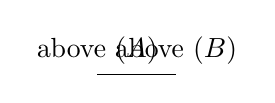
\begin{tikzpicture}
 \coordinate [label=above ($A$)] (A) at (0,0);
 \coordinate [label=above ($B$)] (B) at (1,0);
 
 \draw (A) -- (B);
 \end{tikzpicture}
 \item Uma superfície é aquela que só tem comprimento e largura.
 \item Os extremos de uma superfície são linhas.
 \item Superfície plana é aquela, sobre a qual assenta toda uma tinha reta entre dois pontos quaisquer, que estiverem na mesma superfície.
 \item Ângulo plano é a inclinação recíproca de duas linhas, qu se tocam em uma superfície plana, sem estarem em direitura uma com outra (sem estarem sobre uma mesma linha).
 \item Ângulo plano retilíneo é a inclinação recíproca de duas linhas retas, que se encontram, e não estão em direitura uma com outra.
 \item Um ângulo é a inclinação mutua de duas linhas que se encontram em um plano e não são colineares.
 \item Quando as línhas que compreendem o 

\end{enumerate}%História da Matemática



\bibliographystyle{apa}
\bibliography{referencias}

\end{document}

%http://www.vivendoentresimbolos.com/2014/10/curso-calculo-aula-2-produtos-notaveis-fatoracao-funcoes-transcendentais.html